\documentclass[a4paper,oneside,openany,11pt]{book}
\usepackage{graphicx}
\usepackage{textcomp}
\usepackage{amsmath}
\usepackage{amssymb}
\usepackage[numbers,sort&compress,super,sectionbib]{natbib}
\usepackage{url}
\usepackage{program}
%%\usepackage{palatcm}
\usepackage{engord}
\usepackage{titlesec}
\usepackage[english]{babel}
\usepackage{setspace}
\usepackage{geometry}
\usepackage{fancyhdr}
\usepackage[pdftex,breaklinks=true,citecolor=black,linkcolor=black,urlcolor=black, colorlinks=true,baseurl=http://]{hyperref}
\usepackage{nomencl}
\usepackage{makeidx}

\usepackage{mathpazo}
\linespread{1.05}        % Palatino needs more leading
\usepackage[scaled=0.87]{berasans}
\usepackage[scaled=0.87]{beramono}

\newcommand{\captionfonts}{\footnotesize}
\titleformat{\section}{\small\bfseries}{\thesection}{1em}{}
\titleformat{\subsection}{\small\bfseries}{\thesubsection}{1em}{}

\newenvironment{abstract}%
{\cleardoublepage\null\vfill\thispagestyle{plain}\begin{center}%
\bfseries\abstractname\end{center}}%
{\vfill\null}

\makeatletter

\def\qualification#1{\def\@qualification{#1}}
\def\university#1{\def\@university{#1}}
\def\department#1{\def\@department{#1}}

\long\def\@makecaption#1#2{%
  \vskip\abovecaptionskip
  \sbox\@tempboxa{{\captionfonts #1: #2}}%
  \ifdim \wd\@tempboxa >\hsize
    {\captionfonts #1: #2\par}
  \else
    \hbox to\hsize{\hfil\box\@tempboxa\hfil}%
  \fi
  \vskip\belowcaptionskip}

\renewcommand{\@biblabel}[1]{\quad#1.}
\def\s@btitle{\relax}
\def\subtitle#1{\gdef\s@btitle{#1}}
\def\maketitle{%
  \newpage
  \thispagestyle{empty}
  \null
  \vskip 10em%
  \begin{center}%
  \let \footnote \thanks
    {\LARGE \@title \par}%
		\if\s@btitle\relax
		\else\typeout{[subtitle]}%
			\vskip .5pc
			\begin{large}%
				\textsl{\s@btitle}%
				\par
			\end{large}%
		\fi
    \vskip 1.5em%
    {\large
      \lineskip .5em%
      \begin{tabular}[t]{c}%
	\@author
      \end{tabular}\par}%
    \vskip 1em%
    {\normalsize
      \lineskip .5em%
      \begin{tabular}[t]{c}%
	\@qualification
      \end{tabular}\par}%
    \vskip 1em%
    {\normalsize
      \lineskip .5em%
      \begin{tabular}[t]{c}%
	\@university
      \end{tabular}\par}%
    \vskip 1em%
    {\normalsize
      \lineskip .5em%
      \begin{tabular}[t]{c}%
	\@department
      \end{tabular}\par}%
    \vskip 1em%
    {\normalsize \@date}%
  \end{center}%
  \par
  \vskip 1em}

\def\cleardoublepage{\clearpage\if@twoside
\ifodd\c@page
\else\hbox{}\thispagestyle{empty}\newpage
\if@twocolumn\hbox{}\newpage\fi\fi\fi}

\renewenvironment{thebibliography}[1]
     {\chapter*{\bibname}
      \@mkboth{\MakeUppercase\bibname}{\MakeUppercase\bibname}%
      \list{\@biblabel{\@arabic\c@enumiv}}%
           {\settowidth\labelwidth{\@biblabel{#1}}%
            \leftmargin\labelwidth
            \advance\leftmargin\labelsep
            \@openbib@code
            \usecounter{enumiv}%
            \let\p@enumiv\@empty
            \renewcommand\theenumiv{\@arabic\c@enumiv}}%
      \sloppy
      \clubpenalty4000
      \@clubpenalty \clubpenalty
      \widowpenalty4000%
      \sfcode`\.\@m}
     {\def\@noitemerr
       {\@latex@warning{Empty `thebibliography' environment}}%
      \endlist}

\makeatother
\newcommand{\cNO}{\textrm{NO}}
\newcommand{\cNitrite}{\textrm{NO}$_{\textrm{2}}$$^{\textrm{-}}$}
\newcommand{\cOxygen}{\textrm{O}$_{\textrm{2}}$}
\newcommand{\cNtwoO}{\textrm{N}$_{\textrm{2}}$\textrm{O}}
\newcommand{\Nm}{\textit{N. meningitidis}}
\newcommand{\Nsm}{\textit{Neisseria meningitidis}}
\geometry{a4paper,left=40mm,right=20mm, top=25mm, bottom=25mm}

\renewcommand{\topfraction}{0.85}
\renewcommand{\textfraction}{0.1}
\renewcommand{\floatpagefraction}{0.75}

\title{Analysis and modelling of respiratory metabolism in \Nsm}
\subtitle{}
\author{Andrew Schofield}
\qualification{PhD}
\university{The University of York}
\department{Biology}
\date{March 2012}

\pagestyle{fancy}
\fancyhf{}
\fancyfoot[R]{\textbf{\thepage}}
\renewcommand{\headrulewidth}{0pt}
\fancypagestyle{plain}{%
\fancyhf{} % clear all header and footer fields
\fancyfoot[R]{\textbf{\thepage}} % except the right
\renewcommand{\headrulewidth}{0pt}}


\hyphenation{li-po-po-ly-sacc-har-ides se-ro-groups}
\bibliographystyle{unsrtPLoS-Biology}

\makenomenclature
\makeindex

\begin{document}

\frontmatter
\mainmatter
\maketitle

\cleardoublepage

\begin{abstract}
 
\end{abstract}

\tableofcontents
\listoffigures
\listoftables

\onehalfspacing

\chapter*{Acknowledgements}


\chapter{Introduction}

\section{Biology and pathology of \Nsm}
\Nsm\space is a Gram-negative, bean-shaped diplococcal bacteria \cite{MarcelvanDeuren01012000}, surrounded by a lipid membrane containing outer membrane proteins and lipopolysaccharides \cite{MarcelvanDeuren01012000}. When pathogenic, the bacteria also has a polysaccharide capsule attached to the membrane \cite{MarcelvanDeuren01012000}. It is non-spore forming, non-motile but piliated, and lives as a parasite, with humans being its only host \cite{Stephens2009B71}. \Nm\space inhabits the mucosal membranes primarily in the respiratory tract, and it is estimated that up to 20-25\% of the population have this bacteria in their nasopharynx while being asymptomatic \cite{NancyE.Rosenstein05032001,Stephens2009B71,IWDeVoe06011982}.

The \textit{Neisseria} genus contains a number of non-pathogenic species which are part of the normal human flora including \textit{N. subflava},  \textit{N. flavescens} and \textit{N. lactamica}. Two species of \textit{Neisseria} are the causative agents of human diseases, \Nm, which causes bacterial meningitis and \textit{N. gonorrhoea} which causes gonorrhoea. Being $\beta$-proteobacteria \cite{Stephens2009B71}, the \textit{Neisseria} genus is also related to a number of other pathogenic bacteria including \textit{Bordetella} and \textit{Burkholderia}. This taxa also includes nitrogen-fixing bacteria such as \textit{Nitrosomonas} \cite{Madigan2005}.

\Nm\space is classified into 13 different serogroups based on the differences in lipopolysaccharides, capsules, outer membrane proteins and adhesion molecules \cite{Stephens2009B71,MarcelvanDeuren01012000,Carbonnelle2009B78}. 3 of these 13 serogroups are the main cause of meningococcal meningitis, with serogroups B and C being the most prevalent \cite{MarcelvanDeuren01012000}. Vaccines for Serogroup C are available, but serogroup B currently has no effective vaccine, as it mimics human antigens \cite{Stephens2009B71}. In addition to being the causative agent for meningococcal meningitis, \Nm\space also causes septicaemia and the combination has a mortality rate of ~10\% \cite{MarcelvanDeuren01012000,Stephens2009B71}.

Meningitis is caused by \Nm\space entering the bloodstream and travelling to the meninges, a set of membranes that envelope the central nervous system, where the bacteria goes on to cause inflammation. Once it has entered the bloodstream, \Nm\space is capable of switching its capsule by phase-variation to avoid host-immune detection \cite{AmandaJBeddek05182009,Moxon199424}. After colonisation by the bacterium, in order to enter the bloodstream, it must first adhere to the mucosal tissue. This is facilitated by adhesion molecules on the outer membrane and by pili, with the latter being the primary source of adhesion \cite{MarcelvanDeuren01012000,Carbonnelle2009B78}. Once the bacteria are adhered to the mucosal cells, additional contacts are made with the outer membrane proteins. Interestingly, the presence of the polysaccharide capsule, which is required for survival in the bloodstream, interferes with these additional contacts \cite{Stephens2009B71}. \Nm\space invades the bloodstream by being endocytosed by the mucosal epithelial cells, a process which is triggered by the pili and outer membrane proteins on the bacteria.

\Nm\space is able to survive in the bloodstream (typically an antimicrobial environment) mainly by virtue of its polysaccharide capsule as this is able to protect the bacteria against various immune responses by the host including complement-mediated bacteriolysis and phagocytosis by neutrophils \cite{MarcelvanDeuren01012000}.
%\textit{Neisseria sp.} are also capable of capturing iron directly from the host via transferrins \cite{FSArchibald10011978,DonnaPerkins-Balding03012004}.
 Despite these protective features, specific antibodies \textit{do} provide full protection against the bacteria, but the time taken for these antibodies to be produced means that the host has a period of at least 1 week in which it must rely on innate immune response \cite{MarcelvanDeuren01012000}. Evidence suggests that systemic infection by \Nm\space can only occur in hosts which are immunocompromised in some way, specifically if they do not have the serum bactericidal antibodies against capsular or non-capsular antigens, or they are missing certain complement components \cite{IWDeVoe06011982}. A number of factors can increase the likelihood of contracting bacterial meningitis including smoking and travelling to epidemic regions \cite{Stephens2009B71}. In developed countries, the highest rates of invasive meningococcal meningitis are seen in infants and children less than 4 years-old, adolescents, military recruits and groups where crowding and new exposures occur such as college students living in dormitories, however the disease is capable of affecting all age groups \cite{Stephens2009B71}.

There is evidence to suggest that much of the damage done to the host during a meningococcal infection is actually caused by the host in an attempt to rid itself of the bacteria \cite{NPathan07012003}. A systemic infection causes a massive inflammatory response and the resulting quantities of cytokines produced eventually lead to organ dysfunction and the proteases produced by neutrophil activation also lead to endothelial injury \cite{NPathan07012003}.

Once \Nm\space has entered the bloodstream, it goes on to invade the cerebro-spinal fluid (CSF\nomenclature{CSF}{Cerebrospinal Fluid}), which serves as an excellent culture medium for the bacteria \cite{IWDeVoe06011982}. The host response to this infection is inflammation of the meninges, the membranes surrounding the central nervous system. This leads to a build-up of serous fluid in the brain causing cerebral swelling. Once the bacteria have entered the CSF, antimicrobial treatment is required otherwise the effects are almost invariably fatal \cite{IWDeVoe06011982}.

Initially a meningococcal infection presents as a slight fever and chills, which may improve after 4-6 hours. Hemorrhagic skins lesions may appears between 8 and 18 hours, however roughly 20\% of suffers never present with lesions. These skin lesions are possibly the most well known symptom of bacterial meningitis as they are characterised as a non-blanching (does not turn white under mild pressure) rash. The clearest evidence for meningococcal infection is a fever, stiff neck, aversion to bright light, vomiting, skin lesions and headaches. Unfortunately not all these symptoms may be present in all cases \cite{IWDeVoe06011982}.

When meningococcal septicaemia occurs, renal function may be impaired as a direct consequence of cardiac impairment. Septicaemia causes ``capillary leak'' which reduces cardiac output and increases the effort required to breathe normally. Reduced cardiac output can also affect the gastrointestinal tract leading to reduced function. Once treated these symptoms will usually subside as cardiac output improves \cite{NPathan07012003}.

In most cases the treatment for meningococcal meningitis is with antibiotics, where the primary aim is to achieve a rapid bactericidal effect in the CSF \cite{MarcelvanDeuren01012000}. This treatment is suggested prior to positive identification of cultures of the bacteria obtained from the CSF as any delay is potentially life-threatening if the bacteria have indeed invaded the CSF \cite{IWDeVoe06011982}.

\section{Organisation of the respiratory chain of \Nm}

\Nm\space is classified as an aerobe and as such has an oxidase pathway for reducing oxygen (\cOxygen), but given that the environment in the nasopharynx is poor in oxygen, the bacteria must also be capable of respiring in a microaerobic environment. This is evidenced by the fact that bacterial isolates from the nasopharynx routinely contain both strict aerobes and strict anaerobes \cite{Rock2005}. Genomic analysis of 2 strains of \Nm\space shows that there are 3 terminal oxidases; 1 of each for reducing oxygen, nitrite (\cNitrite) and nitric oxide (\cNO) \cite{Rock2005a}. This analysis may be expanded as there are now many more genomes published. Experiments showed that under oxygen limiting conditions, \Nm\space was capable of growth when nitrite was present in the media (Muller-Hinton Broth), and that nitrate (NO$_{\textrm{3}}^{\textrm{-}}$), the probable source for nitrite, had no effect on growth \cite{Rock2005a}. Additionally the bacteria require carbon dioxide, as shown by \citet{Tuttle1952} and have 2 enzymes which catalyse the reduction of CO$_{\textrm{2}}$ \cite{IWDeVoe06011982}.

\textit{In vivo}, nitrite is obtained as a product of digesting nitrate in food. There are a number of nitrate reducing enzymes present in the mouth and pharynx responsible for this \cite{Rock2005}. Nitrite is also created by oxidation of nitric oxide, which is produced as a host signalling molecule and as a toxin as part of the host immune response \cite{Lundberg2004,Rock2005}.

The respiratory pathway for reducing nitrite in \Nm\space involves 2 steps; nitrite is reduced to nitric oxide, which is then further reduced to nitrous oxide. This represents incomplete reduction, as a further reduction step would reduce nitrous oxide to dinitrogen gas \cite{Rock2005,Deeudom2006}.

Reduction of oxygen is favourable over nitrite reduction due to the redox potential differences. The redox potential of \cOxygen/H$_{\textrm{2}}$O is $+820mV$, \cNitrite/\cNO\space is $+348mV$, thus \cOxygen\space has a higher tendency to acquire electrons resulting in a electrochemically favourable reaction \cite{Deeudom2007}. The electron flow towards the oxidase is also preferred physiologically as it liberates more energy by virtue of the translocation of more protons than the reduction of nitrite. The translocated protons are ultimately used in the synthesis of ATP molecules for energy. This results in reduction of oxygen in preference to nitrite when both are present (in most cases).

Reduction of oxygen in \Nm\space is carried out by the oxygen reductase (oxidase) cytochrome \textit{cbb$_{\textrm{3}}$}, a membrane-bound heme-copper oxidase \cite{Preisig1996}. \textit{cbb$_{\textrm{3}}$} is capable of binding oxygen and nitric oxide, which means that during nitrite reduction (denitrification), the oxidase can be competitively inhibited (chemically) by the intermediate product of denitrification. \textit{cbb$_{\textrm{3}}$} can be permanently damaged at high concentrations of \cNO\space and \cOxygen, as they can both bind at the \textit{cbb$_{\textrm{3}}$} active site and react together to form peroxynitrite \cite{Brown1994295,Sharpe1998,MunaF.Anjum06012002}.

Nitrite is reduced by the nitrite reductase AniA, which is a copper containing reductase. This reduction does not involve translocation of protons, and thus does not produce any useable energy. Nitrite is reduced to nitric oxide which can then be further reduced by a nitric oxide reductase NorB. Since \Nm\space is capable of reducing nitric oxide, a host toxin, directly, this may help it defend itself against part of the host immune response \cite{Heurlier2008,Rock2005} as has been shown in tissue culture by \citet{MunaF.Anjum06012002}.

The reduction processes carried out by these enzymes are shown in the table in Table ~{\ref{tab:reduction-enzymes}}.

\begin{table}[here]
\begin{center}
\begin{tabular}{lcl|l}
\multicolumn{3}{c}{\textbf{Reduction}}& \textbf{Enzyme} \\
\hline
\cNitrite & $\rightarrow$ & \cNO & AniA \\
\cNO & $\rightarrow$ & \cNtwoO & NorB \\
\cOxygen & $\rightarrow$ & H$_{\textrm{2}}$O & \textit{cbb$_{\textrm{3}}$} \\
\end{tabular} 
\end{center}
\small{\caption{The reductions catalysed by the respiratory enzymes in \Nm}}
\label{tab:reduction-enzymes}
\end{table}

The major source for electrons in both respiratory pathways is NADH, although electrons can also be obtained from pyruvate and lactate amongst others. These reduced substrates lead to reduction of ubiquinone to ubiquinol in the ubiquinone pool that exists within the bacteria. Ubiquinol is oxidised either by the cytochrome \textit{bc$_{\textrm{1}}$} complex or directly by the NorB enzyme whilst reducing \cNO\space to \cNtwoO. Cytochrome \textit{bc$_{\textrm{1}}$} is oxidised by a number of intermediate cytochromes which act to transport electrons to the terminal oxidases; AniA and \textit{cbb$_{\textrm{3}}$}. The \textit{c$_{\textrm{5}}$} cytochrome transports electrons from the \textit{bc$_{\textrm{1}}$} complex to AniA, and two cytochromes, \textit{c$_{\textrm{2/x}}$} and \textit{c$_{\textrm{4}}$}, transport electrons to \textit{cbb$_{\textrm{3}}$}. It is not understood why \textit{cbb$_{\textrm{3}}$} has 2 alternate cytochromes, and there is evidence to suggest that it can also be supplied, in a limited capacity, by the \textit{c$_{\textrm{5}}$} cytochrome as well \cite{Deeudom2008}. The electron transport chain is shown graphically in Figure\ref{fig:etc}.

\begin{figure}
 \begin{center}
 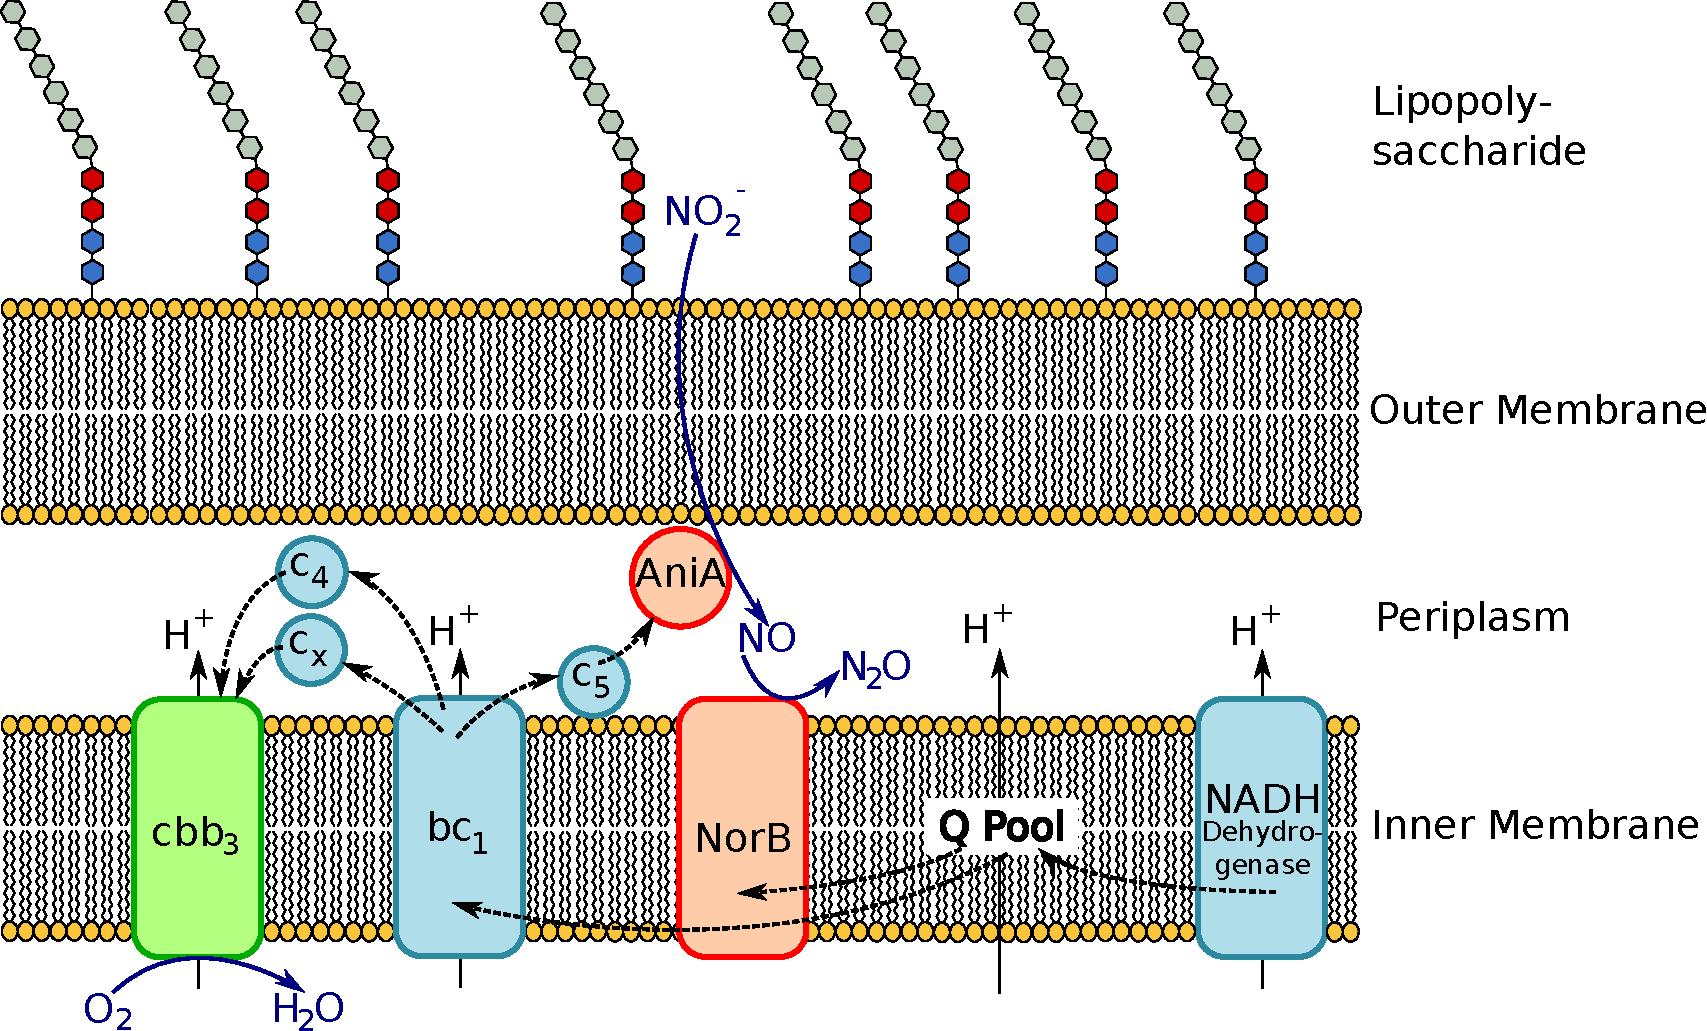
\includegraphics[width=14cm]{./01-introduction/data/Respiratory_layout.pdf}
 % Respiratory_layout.pdf: 819x404 pixel, 72dpi, 28.89x14.25 cm, bb=0 0 819 404
\end{center}
\caption{\footnotesize Layout of the components of the respiratory system in \Nsm. Oxygen reducing components are shown in green, nitrogen reducing components in red. Components transporting electrons are coloured light blue, and their transport is indicated by dashed arrows. Respiratory substrates are shown in dark blue, with corresponding arrows linking them to their reducing enzymes. Components which produce membrane potential are also indicated.}
\label{fig:etc}
\end{figure}

In addition to the difference in favourability between the two respiratory pathways, there is also a great deal of regulation, both at the enzymatic and transcriptional level. Chemical inhibition also plays a part in regulation as briefly mentioned previously. Expression of AniA is regulated by two processes, the reduction of oxygen and the presence of nitrite. The presence of oxygen down-regulates the expression of an activator of AniA expression. This activator is FNR (fumarate and nitrate reduction regulator), and the presence of oxygen effectively means that AniA expression is repressed by the reduced expression of FNR. In \Nm, FNR appears to work slightly differently than in facultative anaerobes such as \textit{E. coli}, in that FNR is still expressed at quite high concentrations of oxygen, and is itself down-regulated by a separate co-factor \cite{Rock2007}.

The presence of nitrite triggers the two component NarP/NarQ system which activates expression of AniA in response to increasing levels of nitrite \cite{Rock2005}. The activity of AniA is also controlled by the competition for electrons by the other reductase enzymes in the respiratory chain. Both NorB and \textit{cbb$_{\textrm{3}}$} have a higher affinity for electrons than AniA, and as a result the presence of these enzymes (when active) has an inhibitory effect on AniA. The regulation of AniA is further complicated by the production of nitric oxide, and the presence of a protein, NsrR.

Nitric oxide has a direct inhibitory effect on the expression of AniA, as does the NsrR protein. Nitric oxide also inhibits the NsrR protein, leading to a de-represssion of AniA \cite{Heurlier2008}. In the absence of nitric oxide, AniA is almost fully repressed by active NsrR. As \cNO\space concentrations increase, NsrR is inactivated allowing full activation of AniA. Once \cNO\space reaches a sufficiently high level it will begin to inhibit AniA \cite{Rock2005,Rock2007}.

NorB is less tightly regulated by respiratory components, as it is only acted upon by NsrR, however it is regulated by FNR and ArsR outside the respiratory chain \cite{VincentIsabella01012008}. This regulation by NsrR works in a similar way to how NsrR acts upon AniA. When there is no nitric oxide present, the NsrR acts to inhibit NorB since there is no substrate for it to reduce. In the presence of nitric oxide, NsrR is inhibited, leading to the activation of NorB which is now able to reduce \cNO\space to \cNtwoO. In this case nitric oxide is acting as a de-repressor of NorB.

This complicated set of regulatory relationships between the different components of the respiratory pathways is shown in Figure \ref{fig:respiratory-pathway}.

\begin{figure}
 \begin{center}
 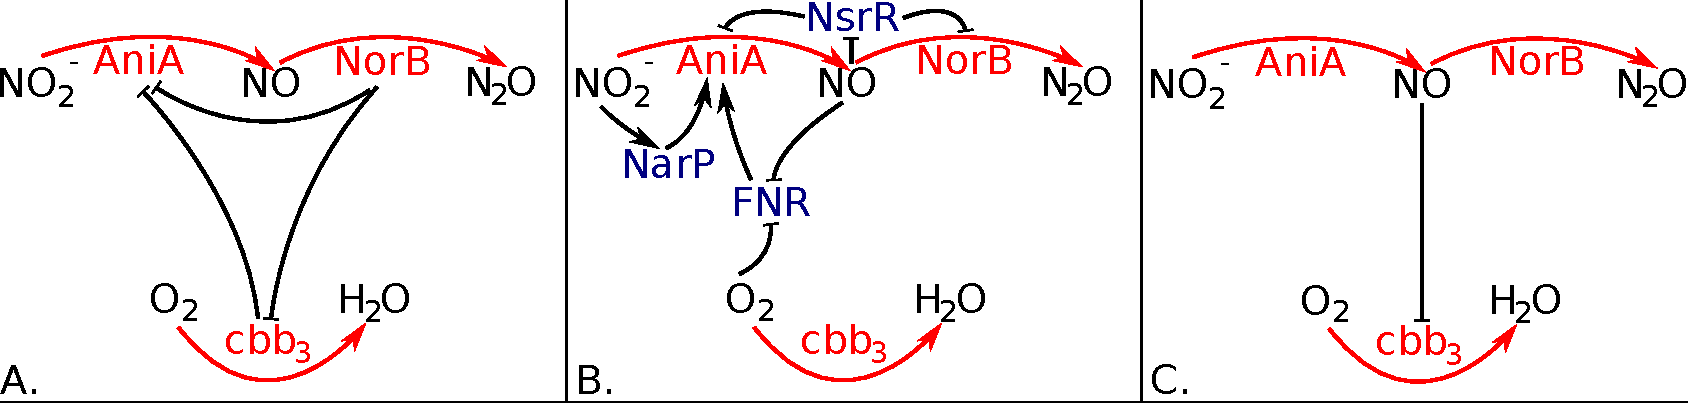
\includegraphics[width=14cm]{./01-introduction/data/regulation.pdf}
\end{center}
\caption{\footnotesize Regulation of respiratory components in \Nsm. Enzymes and enzymatic reactions are shown in red. \textit{A.} describes the regulation caused by competetion for electrons between the respiratory enzymes. \textit{B.} shows the genetic regulation, which also involves a number of additional components in dark blue. \textit{C.} shows chemical inhibition of the respiratory components.}
\label{fig:respiratory-pathway}
\end{figure}

\section{Modelling}

A limited amount of modelling has been carried out on bacterial respiratory chains, these focused on the denitrification pathway and treated the pathway as a simple electrical circuit \cite{almeida_unifying_1997}. An alternative approach involved modeling respiration using ``P systems'' which are probabilistic models of events. This assigned a probability of each reaction happening, dependant on the state of the system and then iterated through a given set of steps evaluating probabilities and altering values based on the outcome \cite{cavaliere_modeling_2006}. This approach to modelling was limited in that it was only predicting the quantities of 1 component in each of 2 ``compartments''; oxygen in the cell membrane and carbon dioxide in the thylakoid membrane (the model was developed using cyanobacteria).

Since when modelling respiration in a cell, the most important factor is the change in concentration of components over time without any particular spatial constraints, ordinary differential equations (ODEs) are an appropriate technique. In these systems the model does not change with regard to the spatial arrangement of any of the components. If the system requires changes in time \textit{and} space, then partial differential equations (PDEs) would be necessary (and more complicated) \cite{Klipp2005}.

Ordinary differential equations only depend on one variable; the time ($t$). In this case, the change in concentration over time for each component can be modelled as a single differential equation. For multiple components this leads to multiple differential equations with some that rely on the result of another (if the rate of one reaction is directly related to the concentration of another component). These ODEs must then be solved in parallel at a suitable timescale.

Complications arise when using differential equations if the processes are considered to be stochastic, as a differential equation model assumes that every component can have a continuous value, which is not the case as molecules are discrete. However if the system being modeled is sufficiently large, this effect can be ignored. If the reaction component size is small ($<$ 100s of molecules) stochastic simulation algorithms have to be used as described by \citet{Gillespie1977}. This method requires far more computation than solving ODEs, as the model will spend most of its time calculating values for reactions involving large molecules even though this is not necessary as the reaction is not stochastic. Additionally, the time interval used between reaction steps is usually very small, meaning the simulation progresses slowly \cite{Klipp2005}.

A number of software packages exist that are capable of this type of modeling such as the Systems Biology Workbench \cite{Sauro2003} and COPASI \cite{StefanHoops12152006}. These allow you to enter biochemical reactions in a format familiar to biologists, and have pre-defined libraries for types of reactions such as mass-action, or one with Michaelas-Menton kinetics etc. The mathematical equations are then derived automatically from the reactions and can be modified by hand if necessary. Parameters for the mathematical equations must be entered, and these will usually be derived from experimental data, or in some cases educated guesses (at least initially). Once a parameter set has been created, the modelling software can run a time-course using a relevant solver-algorithm. COPASI includes 4 solvers,  LSODA (Livermore Solver for Ordinary Differential Equations) \cite{RH93} for deterministic systems (such as ODEs), Gibson-Bruck \cite{Gibson2000} for stochastic systems and Runge-Kutta and LSODA for hybrid systems (where portions are not considered to be stochastic).
\chapter{Materials and Methods}
\label{chap:matandmeth}
\section{\Nsm{} Strains Used in This Work}
\begin{table}[h]
\begin{center}
\begin{tabular}{>{\centering}m{4.4cm}m{6.4cm}>{\centering}m{3.1cm}}
\toprule
\textbf{Name} & \centering \textbf{Description} & \textbf{Source}
\tabularnewline
\midrule
MC58 & Wild-Type Strain & \citet{McGuinness1990}
\tabularnewline\noalign{\smallskip}\hline\noalign{\smallskip}
$\Delta$norB::spc$^\textrm{r}$\nomenclature{spc$^\textrm{r}$}{Spectinomycin resistance} & Wild-Type with insertion of spectinomycin resistance cassette into \textit{norB} gene & \citet{Heurlier2008}
\tabularnewline\noalign{\smallskip}\hline\noalign{\smallskip}
$\Delta$nsrR::spc$^\textrm{r}$ & Wild-Type with insertion of spectinomycin resistance cassette into \textit{nsrR} gene & \citet{Rock2007}
\tabularnewline\noalign{\smallskip}\hline\noalign{\smallskip}
$\Delta$norB::spc$^\textrm{r}$-$\Delta$nsrR::tet$^\textrm{r}$\nomenclature{tet$^\textrm{r}$}{tetracycline resistance} & Wild-Type with insertion of spectinomycin resistance cassette into \textit{norB} and insertion of tetracycline resistance cassette into \textit{nsrR} genes & \citet{Heurlier2008}
\tabularnewline\noalign{\smallskip}\hline\noalign{\smallskip}
$\Delta$aniA::spc$^\textrm{r}$-$\Delta$nsrR::tet$^\textrm{r}$ & Wild-Type with insertion of spectinomycin resistance cassette into \textit{aniA} and insertion of tetracycline resistance cassette into \textit{nsrR} genes & \citet{Heurlier2008}
\tabularnewline
\bottomrule
\end{tabular} 
\end{center}
\caption{Bacterial strains and sources
\label{tab:bacterial-strains}}
\end{table}

\section{Culturing \Nsm{}}
\subsection{Growth of \Nsm{}}
\Nm{} strains were grown on plates on Columbia Agar Base (CAB)\nomenclature{CAB}{Columbia Agar Base} with defibrinated horse blood, and in liquid culture in M\"uller-Hinton Broth (MHB)\nomenclature{MHB}{M\"uller-Hinton Broth}.

Plates were prepared by adding horse blood to a final concentration of 5\% to molten agar, and poured into plastic petri dishes. After streaking with \Nm{} the plates were incubated at 37 \textdegree C in a 5\% carbon dioxide/air mixture.

Aerobic liquid cultures were grown in 10 ml MHB with 10 mM NaHCO$_\textrm{3}$ in plastic sterilin tubes, and incubated at 37 \textdegree C at 200 rpm\nomenclature{rpm}{Revolutions Per Minute}. Microaerobic cultures were suspended in 20 ml MHB, 10 mM NaHCO$_\textrm{3}$ in plastic sterilin tubes, incubated at 37 \textdegree C at 100 rpm.

\subsection{Preparation of Antibiotic Selective Media}
Liquid stock solutions of required antibiotics were either added directly to liquid culture, or, if growing on plates, to the molten agar when also adding horse blood. The final concentrations of antibiotics are given in Table \ref{tab:antibiotic-concs}.

\begin{table}[here]
\begin{center}
\begin{tabular}{cc}
\toprule
\textbf{Antibiotic} & \textbf{Final concentration ($\mu$g/ml)} \\
\midrule
Spectinomycin & 50 \\
Tetracycline & 2.5 \\
Chloramphenicol & 50 \\
\bottomrule
\end{tabular} 
\end{center}
\caption{Final antibiotic concentrations
\label{tab:antibiotic-concs}}
\end{table}

\subsection{Preparation of Frozen Bacterial Stocks}
Bacteria were grown in liquid culture until late log phase prior to harvesting. Liquid cultures were then centrifuged at 4000 g for 15 minutes, and the pellet was then resuspended in a 25\% glycerol, 25\% water and 50\% MHB, all of which had been autoclaved beforehand. The bacterial stocks were then frozen at $-80$ \textdegree C.

\subsection{Streaking Plates for OD to CFU Ratio Calculation}
Bacterial cultures were grown overnight and then transferred into aerobic liquid culture and samples taken throughout the day to obtain a range of different optical densities. The optical density was recorded at 600 nm on a Jenway 6305 Spectrophotometer (Bibby Scientific Limited, Staffordshire UK), and each sample was serially diluted to the following levels: $10^{-5}$, $10^{-6}$ and $10^{-7}$. 100 $\mu$l of each of these dilutions was plated on a fresh blood agar plate and left to grow overnight. The following morning the number of colonies on each plate was counted and used to create a simple conversion factor for Optical Density\nomenclature{OD}{Optical Density} to Colony Forming Units\nomenclature{CFU}{Colony Forming Units}.

\section{Measuring Oxygen Concentration}
Oxygen concentration in respiring cultures was measured using a Clark electrode \cite{Clark1953} from Rank Brothers, Cambridge, UK. This electrode has a silver anode and a platinum cathode and uses a saturated potassium chloride solution as electrolyte. The electrode is set at the bottom of a ~7 ml reaction chamber separated from its contents by a thin Teflon\texttrademark{} membrane. This apparatus is shown in Figure \ref{fig:oxyexpp}. The Teflon\texttrademark{} membrane is permeable to dissolved oxygen, which is reduced by the electrode producing a measurable electrical current. The reaction chamber is maintained at $37$ \textdegree C by an attached water bath.
When performing experiments, 5 ml of culture is added to the reaction chamber, which is stirred by use of a magnetic flea, and the chamber covered with a plastic stopper. The stopper has a number of holes through which the NO probe, or Hamilton syringe can be inserted. Data is collected by attaching the electrode to an external data logger (Pico ADC20, Pico Technology).

\begin{figure}[tbp]
	\begin{center}
		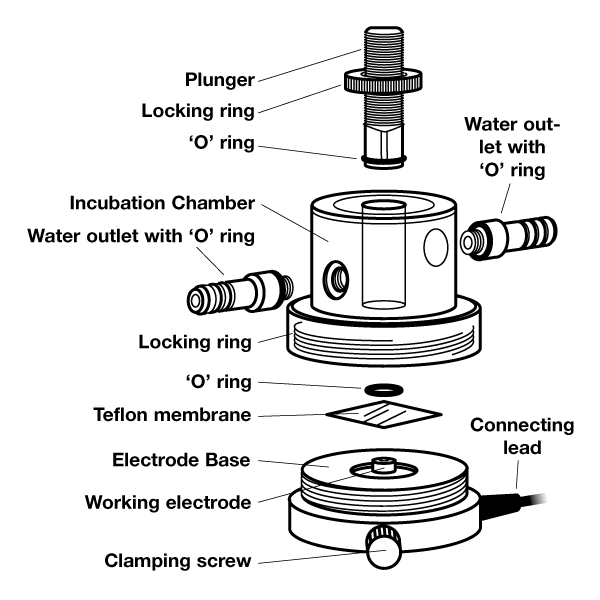
\includegraphics[height=10cm]{02-materialsmethods/data/oxyexpp.png}
	\caption[Exploded view of the oxygen electrode]{{\bf Exploded view of the oxygen electrode.} This assembly sits atop a Rank Brothers Digital Model 10 Controller which acts as a magnetic stirrer and provides the polarising voltage to the electrode (\citet{Rank2012}).
	\label{fig:oxyexpp}}
	\end{center}
\end{figure}


\subsection{Calibration of Oxygen Electrode}
Calibration of the oxygen electrode assumes that anaerobic water will not produce any measurable current at the electrode. Oxygen saturated water contains 210 $\mu$M Oxygen at 37 \textdegree C \cite{YSI2012}. 5 ml of ultra pure ($18~M\Omega$) water was added to the electrode chamber, and then aerated to saturation by use of a pasteur pipette. The maximum value recorded by the data logger then corresponds to a concentration of 210 $\mu$M Oxygen, with the relationship between mV as recorded against concentration being linear.

\section{Measuring Nitric Oxide Concentration}
Nitric Oxide concentration was measured using a Nitric Oxide probe (ISO-NOP, World Precision Instruments) connected to a Nitric Oxide Meter (ISO-NO mkII, World Precision Instruments). This is also a Clark type electrode, contained within a steel sleeve with a semi-permeable membrane separating the working electrode from the system being measured\cite{Liu2005,Bedioui2003,Serpe2007}. The NO probe is inserted through one of the holes in the plastic lid of the reaction chamber of the oxygen electrode assembly. The tip of the electrode should be immersed in the culture, with care being taken not to trap any air bubbles on the surface of the probe. The sensor is also attached to the same data logger as above. In this way both Oxygen and Nitric Oxide concentrations can be measured in parallel. A diagram of the apparatus when set up is shown in Figure \ref{fig:electrode_chamber}.

\begin{figure}[tbp]
 \begin{center}
 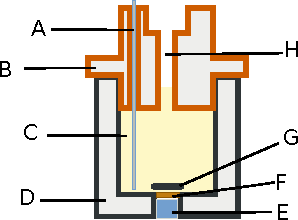
\includegraphics[width=10cm]{./02-materialsmethods/data/electrode_chamber.pdf}
 % electrode chamber.pdf: 595x842 pixel, 72dpi, 20.99x29.70 cm, bb=0 0 595 842
 \caption[Oxygen electrode chamber with nitric oxide probe inserted]{{\bf Oxygen electrode chamber with nitric oxide probe inserted.} This shows the set up used to obtain all oxygen and nitric oxide measurements. A - ISO-NOP Nitric Oxide probe. B - Electrode chamber cap. C - Culture media. D - Oxygen electrode chamber. E - Oxygen working electrode. F - Teflon\texttrademark{} membrane. G - Magnetic Flea. H - Air gap.
 \label{fig:electrode_chamber}}
 \end{center}
\end{figure}


\subsection{Calibration of Nitric Oxide Electrode}
Calibration of the nitric oxide electrode relies on adding known quantities of Nitric Oxide to the electrode chamber. Sodium Nitrite will liberate Nitric Oxide with a 1:1 ratio when added to a solution of excess Potassium Iodide and Sulfuric acid based on the following reaction:

\begin{equation}
2\mathrm{NaNO}_2 + 2\mathrm{KI} + 2 \mathrm{H}_2\mathrm{SO}_4 \longrightarrow 2\mathrm{NO} + \mathrm{I}_2 + 2\mathrm{H}_2\mathrm{O} + 2\mathrm{Na}_2\mathrm{SO}_4
\end{equation}
5 ml of 0.1M Potassium Iodide/Sulfuric Acid was added to the electrode chamber and allowed to stabilise. Then, increasing concentrations of Sodium Nitrite solution were successively added to produce a standard curve of Nitric Oxide concentration to recorded electrode mV. The volume and concentrations of Soduim Nitrite added to the electrode chamber are detailed in Table \ref{tab:sodiumnitrite}.

\begin{table}[here]
\begin{center}
\begin{tabular}{ccc}
\toprule
\multicolumn{2}{c}{$\mathbf{NaNO}_2$} & \textbf{NO} \\
\textbf{Concentration ($\mu$M)} & \textbf{Volume ($\mu$l)} & \textbf{Concentration (nM)} \\
\midrule
10 & 50 & 99 \\
100 & 25 & 591 \\
100 & 50 & 1561 \\
\bottomrule
\end{tabular} 
\end{center}
\caption{Sodium Nitrite concentrations used to calibrate ISO-NOP Nitric Oxide sensor.
\label{tab:sodiumnitrite}}
\end{table}

\section{Measuring Nitrite Concentration (Griess Assay)}
Nitrite concentration in liquid culture was determined using the colorimetric assay described by \citet{DonaldNicholas1957}. This reaction is based on chemical diazotization which uses sulfanilamide and \textit{N}-1-napthylethylenediamine dihydrochloride (NED)\nomenclature{NED}{\textit{N}-1-napthylethylenediamine dihydrochloride} under acidic (hydrochloric acid) conditions. Nitrite is converted to nitrous acid under acidic conditions and this then forms a diazonium salt with the sulfanilamide. The diazonium salt combines with NED and forms a pink azo dye which can be detected using absorbance spectrophotometry at a wavelength of 540 nm. Depending on the expected concentration of nitrite, different sample volumes are used in the assay. The most common sample volume used was $25~\mu\textrm{l}$ which allows detection up to around 1 mM nitrite with the following reagent volumes: $875~\mu\textrm{l}$ of 1\% sulfanilamide in 1 M HCl and $100~\mu\textrm{l}$ of 0.02\% NED in 1 M HCl. When using different sample volumes, the volume of sulfanilamide was altered such that the volume of sample + sulfanilamide always equalled $900~\mu\textrm{l}$. After adding the sample to the reagents, it was left for 20 minutes for the colour to develop, then the absorbance at 540 nm was measured and compared to a standard curve.

\section{Nitric Oxide Production}
Solutions of Nitric Oxide were prepared using a method derived from one described by \citet{Aga2008}. The apparatus setup is shown in Figure \ref{fig:nomaker}. 
\begin{figure}[tbp]
 \centering
 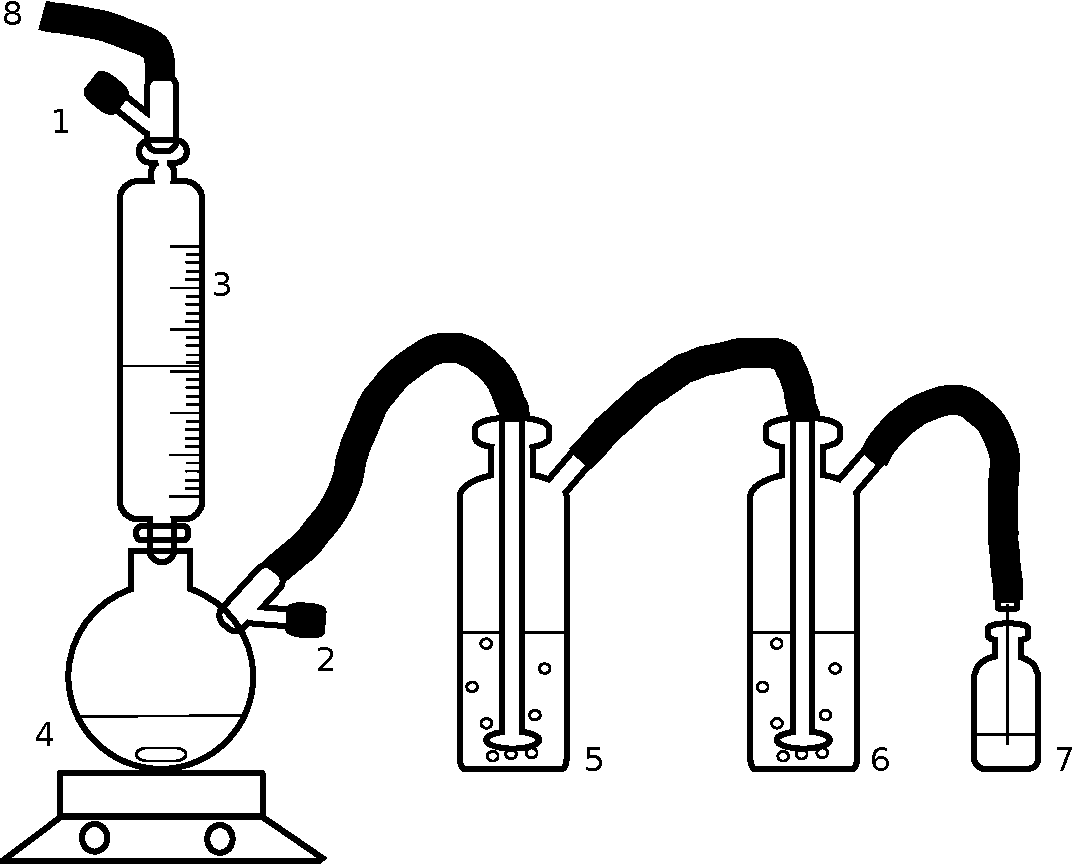
\includegraphics[height=10cm]{./02-materialsmethods/data/drawing.pdf}
 % drawing.pdf: 515x415 pixel, 72dpi, 18.17x14.64 cm, bb=0 0 515 415
 \caption[NO making apparatus.]{{\bf NO making apparatus.} 1 \& 2 - N$_{\textrm{2}}$ release valves. 3 - Pressure equalizing dropping funnel, containing 50 ml 4 M H$_{\textrm{2}}$SO$_{\textrm{4}}$. 4 - Stirred, round-bottomed flask, containing 200 ml 2 M NaNO$_{\textrm{2}}$. 5 - Dreschel bottle with sintered bulb, containing $\approx$ 200 ml 1 M NaOH ($\frac{2}{3}$ full). 6 - Dreschel bottle with sintered bulb, containing $\approx$ 200 ml dH$_{\textrm{2}}$O ($\frac{2}{3}$ full). 7 - Small glass bottle with rubber septum and needle entry valve, containing dH$_{\textrm{2}}$O $\frac{2}{3}$ full. This bottle either needs to also have a gas exit needle, or at least not be sealed during the process.. 8 - To N$_{\textrm{2}}$ gas bottle. Viton rubber tubing is used for all the flexible hoses in this apparatus.
 \label{fig:nomaker}}
\end{figure}
A concentrated solution of Sulfuric acid is added from a pressure-equalizing dropping funnel to a concentrated solution of Sodium Nitrite solution in a stirred, round-bottomed flask. This releases NO gas which passes through a solution of Sodium Hydroxide to neutralise any Sulfuric acid present, then through distilled water to remove any Sodium Hydroxide before finally being bubbled into a collection vessel with a sealed rubber septum containing distilled water. The concentrations of the chemicals used in this preparation are shown in Table \ref{tab:nomakerchem}.
\begin{table}[here]
\begin{center}
\begin{tabular}{ccc}
\toprule
\textbf{Chemical} & \textbf{Volume (ml)} & \textbf{Concentration (M)} \\
\midrule
$\textrm{NaNO}_2$ & 200 & 2 \\
$\textrm{H}_2\textrm{SO}_4$ & 50 & 4 \\
NaOH & 200 & 1 \\
\bottomrule
\end{tabular} 
\end{center}
\caption{Chemicals needed for preparation of Nitric Oxide solution.
\label{tab:nomakerchem}}
\end{table}\\
The system should be set up in a fume cupboard as shown in Figure \ref{fig:nomaker} and sparged with $\textrm{N}_2$ gas for 15 minutes (the dropping funnel will allow gas to pass into the round bottomed flask even when the bottom valve is closed). The $\textrm{H}_2\textrm{SO}_4$ should be sparged separately. Valve 2 should be left open at all times. After sparging close valve 1 and then add the Sulfuric acid dropwise from the dropping funnel. Brown gas will start to bubble through to the collection vessel. This apparatus should produce enough NO gas to saturate several small (10 ml) collection vessels which should have the needle removed and be sealed once saturated. Once all the Sulfuric acid has been added leave the reaction to finish which could take 1-2 hours. Before disassembly the apparatus should be sparged with $\textrm{N}_2$ gas to remove residual NO gas.

The eventual concentration of NO in the solution will vary depending on the temperature, but at 25 \textdegree{}C in ultra pure ($18~M\Omega$) water the concentration will be between 1.88 and 1.96 mM\cite{Aga2008,Cole2008}.
\svnid{$Id$}
\chapter{Parameter Estimation Methodologies}
\label{chap:paramest}

\section{The Challenge of Parameter Estimation}
Parameter estimation is a technique that attempts to estimate the values of a set of parameters based on measured data. This involves creating an estimator - an algorithm that generates new parameter estimates - and some form of calculation to assess how good the estimate is. The model being discussed in this thesis has a large number of unknown values which need to be estimated and it was not clear what values many of these parameters should take, or even if the initial values used are close to the ``true'' values. Given the nature of biology, point estimates for parameters are not going to be representative of the true state of that parameter, thus the output of the parameter estimation needed to be a probability distribution that reflected the likelihood of the parameter taking on a particular value. Another requirement of the estimator is that it needs to be able to select new estimates based on prior probability distributions, since some information about certain parameters is known beforehand, and this knowledge will improve as more datasets are analysed.

These requirements lends themselves well to Monte-Carlo type methods, which produce output which can be represented as a probability distribution and can be selected from a prior probability distribution.

\section{Methods and Algorithms Used}
Below are the various different methods for parameter estimation that were investigated during the course of this work. All of these methods involve a sampling system that attempts to select parameter values which minimise the difference between the simulation result and the experimental data by using a difference function. The main difference between the parameter estimation methodologies laid out below are the ways in which they generate new parameter values, either from a probability distribution or based on the previous value, and the way this is applied and tested against the experimental data. The aim of the parameter estimation methodology was to achieve an output from the difference function that was as close to zero (perfect fit/no difference) as possible. The value produced by the difference function is hereby referred to as the \textit{Badness of Fit} or \textit{BOF} value, due to larger values representing worse fits to the experimental data.

\subsection{Difference Functions}
Two different difference functions were used to calculate the \textit{BOF} value. One was the sum of the Least Squares Differences between the measured components in the experimental data and the simulation result. This was used in early parameter estimation runs.

\begin{equation}
BOF = \sum^{n}_{j=1}\left(\sqrt{\sum^{m}_{i=1} (\Delta x_{ij})^2}\right)
\end{equation}
Where $j$ is the current parameter, $n$ the number of parameters, $i$ the current data point, $m$ the total number of data points and $(\Delta x_{ij})^2$ the square of the residuals between the experimental and solved data for parameter $j$ at data point $i$. Therefore the \textit{BOF} value becomes ``the sum of the squares of the residuals for each data point for each parameter.''

The second method for calculating the \textit{BOF} was a log-likelihood calculation. This method calculates the likelihood of the solved data falling under a normal distribution which has the experimental data as its $\mu$, and a preset error value as its $\sigma$. The method was used as it allowed tuning of the $\sigma$ value, which provided more control over how new parameter sets were accepted. The lower the value of $\sigma$, the closer the solved data needs to be to the experimental data to achieve a low \textit{BOF} value.

\begin{equation}
BOF = \sum^{n}_{j=1}\left(\sum^{m}_{i=1}\ln(norm(x_1,\mu_1,\sigma)) - \ln(norm(x_2,\mu_2,\sigma))\right)
\end{equation}
Where $j$ is the current parameter, $n$ is the number of parameters, $i$ is the current data point, $m$ is the total number of data points, $norm$ is a function that accepts 3 arguments ($x, \mu, \sigma$) and returns the probability associated with $x$ in a normal distribution with parameters $\mu$ and $\sigma$, $x_1$ and $\mu_1$ are zero, $x_2$ is the solved value at data point $i$ for parameter $j$, $\mu_2$ is the experimental value at data point $i$ for parameter $j$ and $\sigma$ is the preset standard deviation.

$x_1$ and $\mu_1$ are set to zero because this likelihood calculation can also be used on the time axis in addition to the value axis. Since there is no time uncertainty in the data, this can be ignored by setting these values to zero. The value for $\sigma$ is determined such that the first few iterations of parameter estimation generate very high \textit{BOF} values (with the knowledge that this will always decrease) subject to the computational limits imposed by floating point precision (values of $\sigma$ which are too low generate nonsensical \textit{BOF} values).

In most cases the components used for calculating the likelihood are Oxygen and Nitric Oxide, as these were the primary measured chemicals.
\subsection{Monte Carlo Methods}
A brief section is included here to describe Monte Carlo Methods, as the techniques used for parameter estimation all use this method as their estimator in some form.
``Monte Carlo Methods'' is a generalised term to describe a stochastic technique that makes use of random numbers to examine a problem in conjunction with probability statistics. Monte Carlo Methods allow modelling of complex systems without having to exhaustively search every possible outcome. Large systems are sampled in random configurations and that data applied in such a way that it can be used to describe the system as a whole. ``Monte Carlo techniques are often the only practical way to evaluate difficult integrals or to sample random variables governed by complicated probability density functions''\cite{Nakamura2010}. The generalized form of Monte Carlo Methods involves generating a set of random numbers which conform to a particular probability distribution (depending on the problem) and observing the fraction of those numbers which fulfil a particular set of properties (when transformed by some algorithm). The larger the number of random numbers generated, the more useful the output.

As a simple example, the value of $\pi$ can be estimated using a Monte Carlo method. With the prior knowledge that $\frac{\pi}{4}$ is equal to the area of a circle with diameter $d$, divided by the area of a square with sides $d$ (see appendix), the value of $\pi$ can be estimated simply by generating uniformly distributed random points on the square and the counting the number that also lie inside the circle. The value of $\pi$ is $4\times\frac{\mathrm{number~of~points~in~circle}}{\mathrm{total~number~of~points}}$. The estimate for the value of $\pi$ improves with the number of points (and in this case converges slowly on the true value).

\subsubsection{Markov Chain Monte Carlo}
Markov Chain Monte Carlo algorithms use Monte Carlo Methods to create a Markov chain whose stationary distribution is the desired (posterior) distribution. Markov Chains are sequences of states where state $x_{t+1}$ depends only on state $x_t$. Given suitably large numbers of states, the chain will forget the initial state $(x_0)$ and the resulting chain will represent the posterior (stationary) distribution. This distribution won't depend on either $t$ or $x_0$\cite{Gilks1996}. The states in the chain prior to arriving at the stationary distribution are known as ``burn in'' and are discarded, and the stationary distribution is the usable output which can then be converted into a more convenient format to use as a posterior probability distribution.

\subsection{Simulated Annealing}
This technique was described independently by \citet{Kirkpatrick1983} and \citet{Cerny1985}. The name comes from the metallurgical annealing process whereby large crystals are formed while a material is slowly cooled. The slow cooling increases the probability of individual crystals obtaining lower energy states than the initial. As the material cools the ``distance'' each crystal can move along the energy landscape decreases. In a simulated annealing algorithm, ``distance'' is controlled by a perturbation kernel which takes the ``temperature'' as input to change how much each parameter can be perturbed.
Simulated annealing ``consists of a discrete-time inhomogeneous Markov chain''\cite{Bertsimas1993} whereby the previous state is modified with a perturbation kernel (the neighbouring states) and then accepted or rejected using a transition probability which depends on the current temperature and the energies of the previous and current states. The advantage of this scheme is that areas of local minima have a lesser effect on the outcome of the Markov chain as the high initial temperature allows for the chain to ``jump'' out of these minima.
\begin{figure}[tbp]
\small
\begin{verbatim}
c1 = c0;
c2 = mutate(c1);
i = 0;
while i < i_max
  if fitness(c1) > fitness(c2)
    c2 = mutate(c1)
  else
    c1 = mutate(c2)
  i = i + 1
if fitness(c1) > fitness(c2)
  return c1
else
  return c2
\end{verbatim}
\caption[Pseudo-code showing how a rejection sampler works.]{{\bf Pseudo-code showing how a rejection sampler works.}
\label{fig:sa_code}}
\end{figure}

Simulated annealing is an extension of a simple rejection sampler \cite{Marjoram2003}. Figure~\ref{fig:sa_code} contains some simple pseudo-code which shows how the basic rejection sampler algorithm works. This will provide a ``best'' parameter set, but there is no information about the possible spread of values in the parameter set. Given that it is unlikely that a single point-value parameter-set solution exists that will accurately describe the system it is necessary to produce a spread of results that will adequately describe the system instead. To this end a modified version of simulated annealing was used integrated with aspects of a simple genetic algorithm. In the genetic algorithm paradigm a synthetic ``chromosome'' is created which contains ``genes'' representing the parameters in the simulation. These include the rate constants, concentrations of various components and initial concentrations of substrates and products. This chromosome is then copied and perturbed several times (depending on the eventual population size required), with the size of the perturbation being dependent on the current annealing temperature. For instance the highest temperature could indicate that the individual parameters can be perturbed by up to $\pm 10\%$, and as the temperature decreases the perturbation percentage has a concomitant decrease. An example annealing temperature schedule is shown in Figure \ref{fig:temperature}.
\begin{figure}[tbp]
	\begin{center}
		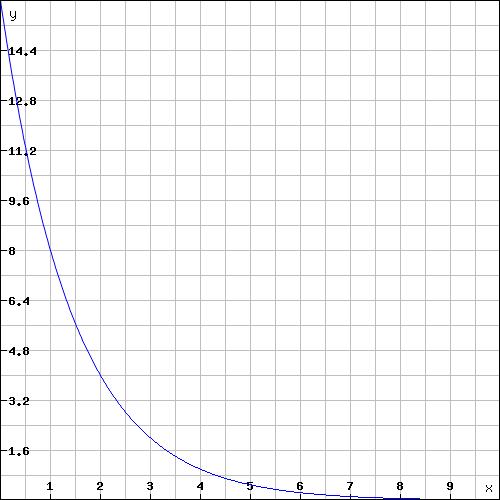
\includegraphics[height=10cm]{03-parameterestimationmethodologies/data/temperature.png}
		%a0=2&a1=1/((2^x)/16)&a2=&a3=&a4=1&a5=4&a6=8&a7=&a8=1&a9=1&b0=500&b1=500&b2=0&b3=10&b4=0&b5=16&b6=10&b7=10&b8=5&b9=5&c0=3&c1=0&c2=1&c3=1&c4=1&c5=1&c6=1&c7=0&c8=0&c9=0&d0=1&d1=20&d2=20&d3=0&d4=&d5=&d6=&d7=&d8=&d9=&e0=&e1=&e2=&e3=&e4=14&e5=14&e6=13&e7=12&e8=0&e9=0&f0=0&f1=1&f2=1&f3=0&f4=0&f5=&f6=&f7=&f8=&f9=&g0=&g1=1&g2=1&g3=0&g4=0&g5=0&g6=Y&g7=ffffff&g8=a0b0c0&g9=6080a0&h0=1&z
	\caption[Example simulated annealing temperature schedule]{{\bf Example simulated annealing temperature schedule.} This represents how the annealing temperature changes as the annealing process progresses. Temperature is denoted by the y-axis value, and simulation progress by the x-axis value. This is a heavily compressed time-frame, as in reality the system would normally process 10,000 sets of parameters at each annealing temperature.
	\label{fig:temperature}}
	\end{center}
\end{figure}
The annealing temperature is programmed to decrease after a defined number of iterations such that the magnitude of individual mutations becomes smaller as the simulation progresses. This should have the effect of honing in on a set of parameters with a better likelihood.
Once the chromosome population has been created, 2 are selected at random and their likelihoods evaluated, in this case by the Least Squares Difference method. The chromosome with the lowest likelihood is discarded and the other is cloned and perturbed. The two chromosomes are then added back to the chromosome population. The genetic algorithm is used to improve the parameters sets by perturbing genes (individual parameters) from fit chromosomes (complete parameter sets), re-running the simulation and discarding unfit parameter sets. An unfit parameter set is defined as one with an likelihood lower than the highest so far. This technique involves having two chromosomes selected at any one time. The parameters from each chromosome are simulated and the least fit one is discarded. At this point the contents from the fitter chromosome are cloned and perturbed, and the cycle is repeated. Figure~\ref{fig:sa_spread} shows this diagrammatically. After many cycles (upwards of 1000) the chromosome pool should only contain the best fitting parameter sets to the experimental data. The spread of the parameters can be used to infer the sensitivity of the simulation to changes in parameter values in a similar way to that described by \citet{Toni2009}.
\begin{figure}[tbp]
\begin{center}
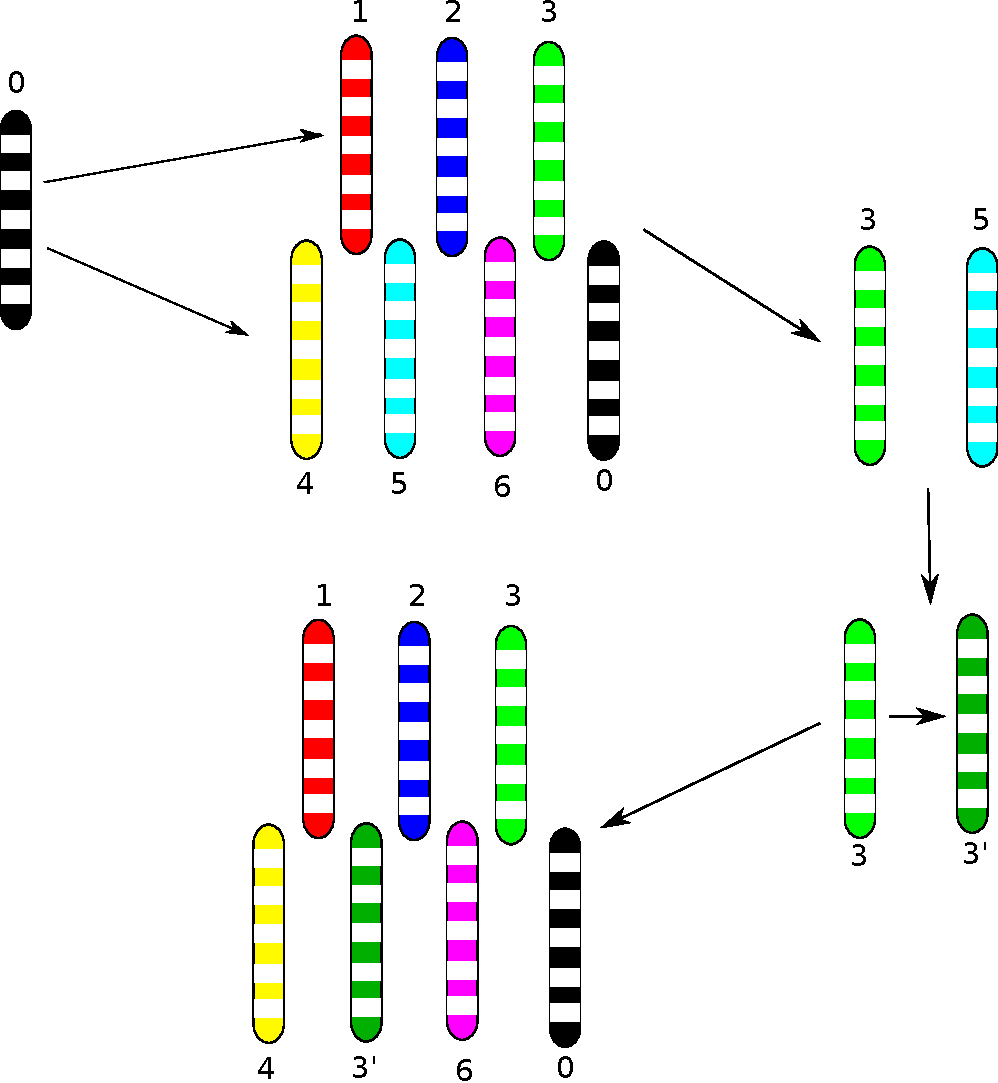
\includegraphics[height=10cm]{./03-parameterestimationmethodologies/data/sa_spread.pdf}
% sa_spread.pdf: 479x520 pixel, 72dpi, 16.90x18.34 cm, bb=0 0 479 520
\end{center}
\caption[{Schematic diagram showing the technique used to generate a spread of parameters using a synthetic chromosome.}]{{\bf Schematic diagram showing the technique used to generate a spread of parameters using a synthetic chromosome.} The parameters are loaded as genes on the chromosome which are then perturbed, 2 chosen and the fittest kept and perturbed. Each time a chromosome is perturbed it is reintroduced into the chromosome pool, and the next 2 chromosomes are chosen at random.
\label{fig:sa_spread}}
\end{figure}
%\textbf{Advantages}
%\begin{itemize}
%	\item Easy to implement.
%	\item Can avoid local energy minima by jumping when the temperature is high.
%	\item Energy need only be calculated for 2 samples at any one time.
%	\item High optimisation performance on some problems.
%\end{itemize}
%\textbf{Disadvantages}
%\begin{itemize}
%	\item Slow performance on certain problems.
%	\item Cannot produce probability distributions.
%\end{itemize}
%\textbf{Reason(s) for rejection}
%\begin{itemize}
%	\item Seemed to be incapable during testing of settling on solutions to Nitric Oxide reduction datasets.
%	\item No probability distributions which were eventually required to incorporate data from previous datasets.
%\end{itemize}

This algorithm was rejected as unsuitable as it seemed to be incapable of settling on solutions to the Nitric Oxide reduction datasets during testing. Additionally this technique does not produce probability distributions which were eventually required to incorporate data from previous datasets.

%The algorithm is flexible in that it includes a gene mask in the chromosome which allows any number of genes to be switched on or off. In this way it is possible to fix the values of certain parameters, and prevent them from being perturbed at each iteration. This is useful during the parameter search process, as a limited dataset can be used, which only describes a limited subset of the overall model, and any parameters which are unrelated to that dataset can be removed. Practically this means it is possible to focus on one particular aspect of the model, such as oxygen utilisation, set all the parameters which are irrelevant to zero, and prevent them from being included in the genetic algorithm. During this process, the parameters related to oxygen utilisation can be improved, and once a sufficient set of value is obtained, these can then be fixed when a different dataset is used, such as \cNO \space reduction.

\subsection{Approximate Bayesian Computation by Sequential Monte Carlo}
``Approximate Bayesian Computation methods have been conceived with the aim of inferring posterior distributions where likelihood functions are computationally intractable or too costly to evaluate. They exploit the computational efficiency of modern simulation techniques by replacing calculation of the likelihood with a comparison between the observed data and simulated data''\cite{Toni2009}.

To incrementally improve the parameter sets, a version of Bayesian inference is used in conjunction with a standard Monte Carlo method in a system called Approximate Bayesian Computation by Sequential Monte Carlo (ABCSMC)\nomenclature{ABCSMC}{Approximate Bayesian Computation by Sequential Monte Carlo} as described by \citet{Toni2009}. An implementation of algorithm (S) was used from that paper.

\textbf{\textit{Bayesian Inference}} - This is a statistical method for inferring the probability of a hypothesis based on available evidence. As more evidence is accumulated, the inference is updated and the probability of the hypothesis being true is changed. Given enough evidence, the probability of the hypothesis being true should either be very high or very low causing you to either accept or reject the hypothesis. Bayesian inference relies on having a prior probability (or probability distribution) for the hypothesis, and this can inevitably introduce a level of bias into the inference.
Bayesian inference can be described thus:
\begin{equation}
P(H\mid E) = \dfrac{P(E\mid H)}{P(E)}\cdot P(H)
\label{eq:bayes}
\end{equation}
\begin{itemize}
	\item $P(H\mid E)$ is the posterior distribution of $H$ given $E$.
	\item $P(H)$ is the prior distribution
	\item $\dfrac{P(E\mid H)}{P(E)}$ is the impact of $E$ on the degree of belief in $H$.
\end{itemize}

A simplistic example of using Bayesian inference to alter a hypothesis could happen in the case of having two jars of sweets. Jar 1 has 15 strawberry sweets and 25 raspberry sweets. Jar 2 has 20 of each. Supposing a third party selects 1 sweet at random from 1 of the jars. They select a strawberry sweet, what is the probability that it came from Jar 1? From the point of view of our third party both jars are identical, therefore $P(H_1) = P(H_2)$ and the total probability must equal 1, so the prior probability of each jar is 0.5. The observation, $E$ is of a strawberry sweet, which we can then use to calculate the likelihood of it being from each jar individually by $P(E\mid H_1) = 15/40 = 0.375$ and $P(E\mid H_2) = 20/40 = 0.5$.
The Generalised Bayes formula can then be used to work out the probability of the strawberry sweet being from jar 1, that is $P(H_1\mid E)$.\\
\begin{align}
\nonumber
P(H_1\mid E) & = \dfrac{P(E\mid H_1)P(H_1)}{P(E\mid H_1)P(H_1) + P(E\mid H_2)P(H_2)}\\
\nonumber \\
\nonumber
& = \dfrac{0.375 \times 0.5}{0.375 \times 0.5 + 0.5 \times 0.5}\\
\nonumber \\
& = 0.429
\end{align}

Before the observation of the sweet, the probability of the third party taking from jar 1 was the prior probability of $0.5$. After the observation this probability must be revised to 0.429.

Bayesian inference is widely used in computational analysis for artificial intelligence and email spam identification. It is also used in the field of population genetics and phylogenetics\cite{Ronquist2011}.

\textbf{\textit{Approximate Bayesian Computation}} - This is an adaptation of Bayesian inference which allows approximately the same inferences to be made, with considerably less computation. It operates on representations of the datasets rather than the datasets themselves. Common examples are population mean and variance. This is useful for large complex datasets where the probability of a simulation of the dataset matching the original is very small (unacceptably so), in this case a representation of the datasets can be used, and the difference calculated. If the difference is less than a pre-defined acceptance threshold, then the simulated dataset is accepted. \nomenclature{ABC}{Approximate Bayesian computation}ABC originally came from the fields of population and evolutionary genetics\cite{Beaumont2002}, but is now being applied to complex and stochastic dynamical systems\cite{Sisson2007,Toni2009,Beaumont2010}.

ABC differs from standard Bayesian inference shown in Equation \ref{eq:bayes} in that the likelihood term does not need to be calculated. Instead the difference between the summary statistics of the observed data and the simulated data is used. The simulated data is considered a true sample from the posterior distribution if the difference in summary statistics is less than a predefined acceptance threshold.
The most basic ABC methods takes the following form:\\
$\theta$ is a parameter vector to be estimated, $\pi(\theta)$ is the prior probability distribution, and $x$ is the observed data. The posterior distribution is $\pi(\theta \mid x) \propto f(x \mid \theta)\cdot \pi(\theta)$.
\begin{enumerate}
	\item Create a candidate parameter vector $\theta^*$ from the prior distribution $\pi(\theta)$.
	\item Simulate dataset $x^*$ using the model and parameter vector $\theta^*$.
	\item Compare $x^*$ with $x$ using a distance function $d$ and an acceptance criteria $\epsilon$. If $d(x,x^*)\leq \epsilon$, accept $\theta$.
\end{enumerate}

Given a low enough value for $\epsilon$, the output distribution should approximate the true posterior distribution if sampled a large enough number of times.

\textbf{\textit{Sequential Monte Carlo}} - This is a method of particle filtering whereby a large set of samples ($N$) are drawn from the prior distribution, and for each sample, the probability is calculated. Weights for each particle are assigned based on the probabilities, and these affect how likely a particle is to be selected in subsequent rounds of selection. At the end of each round, the posterior distribution of the $N$ particles becomes the prior distribution for the next round.

\textbf{\textit{Approximate Bayesian Computation by Sequential Monte Carlo}} - This combines the previous two methods by drawing a large number of particles from the prior distribution using Bayesian inference. The prior distribution is discrete in the scheme used here, so a perturbation kernel based on a Laplacian or Gaussian distribution is used on each sample to provide small deviations to better approximate a continuous prior distribution. Each sample is simulated and only accepted if it exceeds the acceptance threshold. This is calculated based on the \nomenclature{LSD}{Least-Squares Difference}least-squares difference (LSD) between the simulated data and the original dataset. If a sample is rejected, a new one is drawn from the prior distribution and SMC then continues as described above. The weights of the accepted samples are calculated based on the probabilities of being selected from the prior and the samples go on to form the posterior distribution. For each subsequent round, the mean LSD of the posterior distribution from the previous round is used as the acceptance threshold. This ensures that each round results in better fitting parameter sets. The cycle is then repeated until a pre-defined cycle limit is reached \cite{Toni2009}.

A significant advantage of this technique is that it is readily parallelisable, as each particle in the SMC\nomenclature{SMC}{Sequential Monte Carlo} process is independent, thus can be simulated in parallel. A parallel version of this algorithm was implemented in the JAVA programming language which resulted in significant speed-ups when multiple processing threads can be used. The threading manager means that the algorithm is theoretically most efficient (in terms of computational time) when the number of particles is an exact multiple of the number of processing threads. In practice however this is negated by the fact that some particles require multiple samples due to them not meeting the acceptance criteria.

%\textbf{Advantages}
%\begin{itemize}
%	\item Paralellisable. Leading to improved performance on multiprocessor systems.
%\end{itemize}
%\textbf{Disadvantages}
%\begin{itemize}
%	\item Requires a suitable distance function or summary statistic.
%\end{itemize}
%\textbf{Reason(s) for rejection}
%\begin{itemize}
%	\item Seemed incapable of settling on sensible posterior distributions with some datasets. I suspect the distance function used was causing a conflict which meant the algorithm was accepting bad parameter sets and rejecting good ones.
%\end{itemize}

This algorithm was rejected on the grounds that it seemed incapable of settling on sensible posterior distributions with some datasets. It is suspected that the distance function used was causing a conflict which meant the algorithm was accepting bad parameter sets and rejecting good ones. The requirement of a suitable distance function or summary statistic is a major disadvantage of this algorithm.

\subsection{Metropolis Hastings Monte Carlo}
The Metropolis-Hastings algorithm is a Markov Chain Monte Carlo method to retrieve sequences of random samples from a probability distribution which cannot be sampled directly (or would be very difficult) such as when no probability distribution function exists. Such a case exists when the proposal distribution is a discrete rather than a continuous distribution. The algorithm was originally developed by \citet{Metropolis1953} for generating samples from the Boltzmann distribution. It was later extended to a more general form for any distribution by \citet{Hastings1970}.

This algorithm is much simpler than the previously described ABCSMC and takes the following form\cite{Gilks1996}:

\singlespacing %necessary to produce nice code
\begin{alltt}
Initialise \(X_0\); set \(t=0\);
Repeat \{
  Sample a point \(Y\) from \(q(.|X\sb{t})\)
  Sample a Uniform(0,1) random variable \(U\)
  If \(U \leq \alpha(X\sb{t},Y)\) set \(X\sb{t+1}=Y\)
    otherwise set \(X\sb{t+1}=X_t\)
  Increment t
\}
\end{alltt}
\doublespacing %remember to un-single space!

For the parameter estimation problem being solved, in the algorithm above, $X_0$ is the initial set of parameters, $t$ is the iteration number, $q(.\mid X_t)$ is the \textit{proposal distribution} which is the prior probability distribution and $\alpha(X_t,Y)$ is the acceptance probability. The acceptance probability is calculated from the likelihood of $Y$ being from the prior probability distribution and the likelihood of the solved data being from a normal distribution surrounding the experimental data. Mathematically it is described thus:
\begin{equation*}
\alpha(X_t,Y) = \frac{q(Y_t\mid X)}{q(Y_{t-1}\mid X)}\cdot\e{}^{BOF(Y_{t-1}) - BOF(Y_t)}
\end{equation*}
This process can be described as below:
\begin{enumerate}
\item Create a set of starting parameter values, calculate the probability of them from the prior distribution, and their likelihood of fitting the experimental data.
\item Sample new parameter values from the prior probability distribution, calculate probabilities and likelihoods.
\item Calculate acceptance based on the above values.
\item If acceptance is greater than a random number generated in the range 0-1 then save the new parameters. (Acceptance will be greater than 1 if the parameters are more likely \textit{and} the results fit better). This allows slightly less probable, and less likely results to be accepted
\item Otherwise save the old parameters.
\item Go Back to step 2
\item After enough repeats the saved results will resemble the posterior probability distribution.
\end{enumerate}
This was the algorithm selected to perform the parameter estimation as it was simple to implement, generated the required probability distributions and didn't require complex functions to determine acceptance. Its only major disadvantage was that it was an unparallel algorithm, thus it was quite slow as each iteration depended on the results of the previous.

\section{Validating the Parameter Estimation Algorithm}

The Metropolis Hastings Monte Carlo algorithm was validated by using a much simpler ODE system than is required by the respiratory model, to make sure it was capable of parameter estimation and producing the necessary output for creating probability distributions. The simpler ODE system selected was the Lotka-Volterra model as this can be tested much more quickly by virtue of having far fewer parameters to estimate (4 as opposed to \gt 20) and has only 2 differential equations to solve. The Lotka-Volterra model describes a simple predator-prey relationship\cite{Lotka1925,Volterra1931} and only requires two first-order, non-linear differential equations, which are shown in equation \ref{eq:lv}.
\begin{eqnarray}
\frac{dx}{dt} = x (\alpha - \beta y)\nonumber \\
\frac{dy}{dt} = -y (\gamma - \delta x)
\label{eq:lv}
\end{eqnarray}

The algorithm was validated by generating a dataset using the Lotka-Volterra equations with a known set of parameters. The dataset was generated using the same ODE solving equations described in Chapter \ref{chap:model} for 1000 generations. The Metropolis Hastings algorithm was given uniform distributions to sample from for each of the priors (this means that there is more-or-less no sampling distribution), and the acceptance criteria for each iteration were based upon the log-likelihood (described previously) values between the input dataset and the solved output from the new parameters. The algorithm was allowed to continue for 10000 iterations, generating 4 Markov-Chains of length 10000. During this time the algorithm will be altering the 4 input parameters trying to improve them based on the log-likelihood values produced. The resulting Markov Chains represented the stationary or posterior distributions of the 4 parameters and were very close to the true values from the input data.

Given the simplicity of this system, a particularly bad set of initial parameter estimates (i.e. $x_0$ as described previously) were given to exaggerate the burn in period, and to show that given a long enough time the algorithm will eventually settle on ``correct'' values. This validation step also informs the likely values for two tuning variables in the algorithm; the \textit{acceptance} - how stringent the algorithm is on accepting new parameter sets, which is the $\sigma$ value of the log-likelihood calculation, and the \textit{internal sigma} value - this describes the magnitude of parameter perturbation at each iteration.
The graphical results of the Lotka-Volterra validation are shown in Figures \ref{fig:simulation} and \ref{fig:parameters}. Figure \ref{fig:simulation} shows the generated validation data compared to the solved output from the parameters at the end of the Markov Chains. Figure \ref{fig:parameters} shows a plot of the 4 Markov Chains generated by the MHMC algorithm. The initial 3000 generations are the burn-in and represent the region of the Markov Chain where the algorithm is trying to converge on the stationary distribution. The region beyond 3000 generations \textit{is} the stationary distribution and this can be used to calculate a posterior probability distribution (the sampling distribution was flat).

The results of this validation show that the algorithm is capable of parameter estimation and can produce output that is compatible with generating probability distributions. The comparison of the Lotka-Volterra data shows that the algorithm could have been run for more iterations as the solved output doesn't quite match the generated input data. The Markov Chains show that the algorithm has stabilised on values very close to the ``true'' values of the input data.

\begin{figure}[tbp]
 \centering
 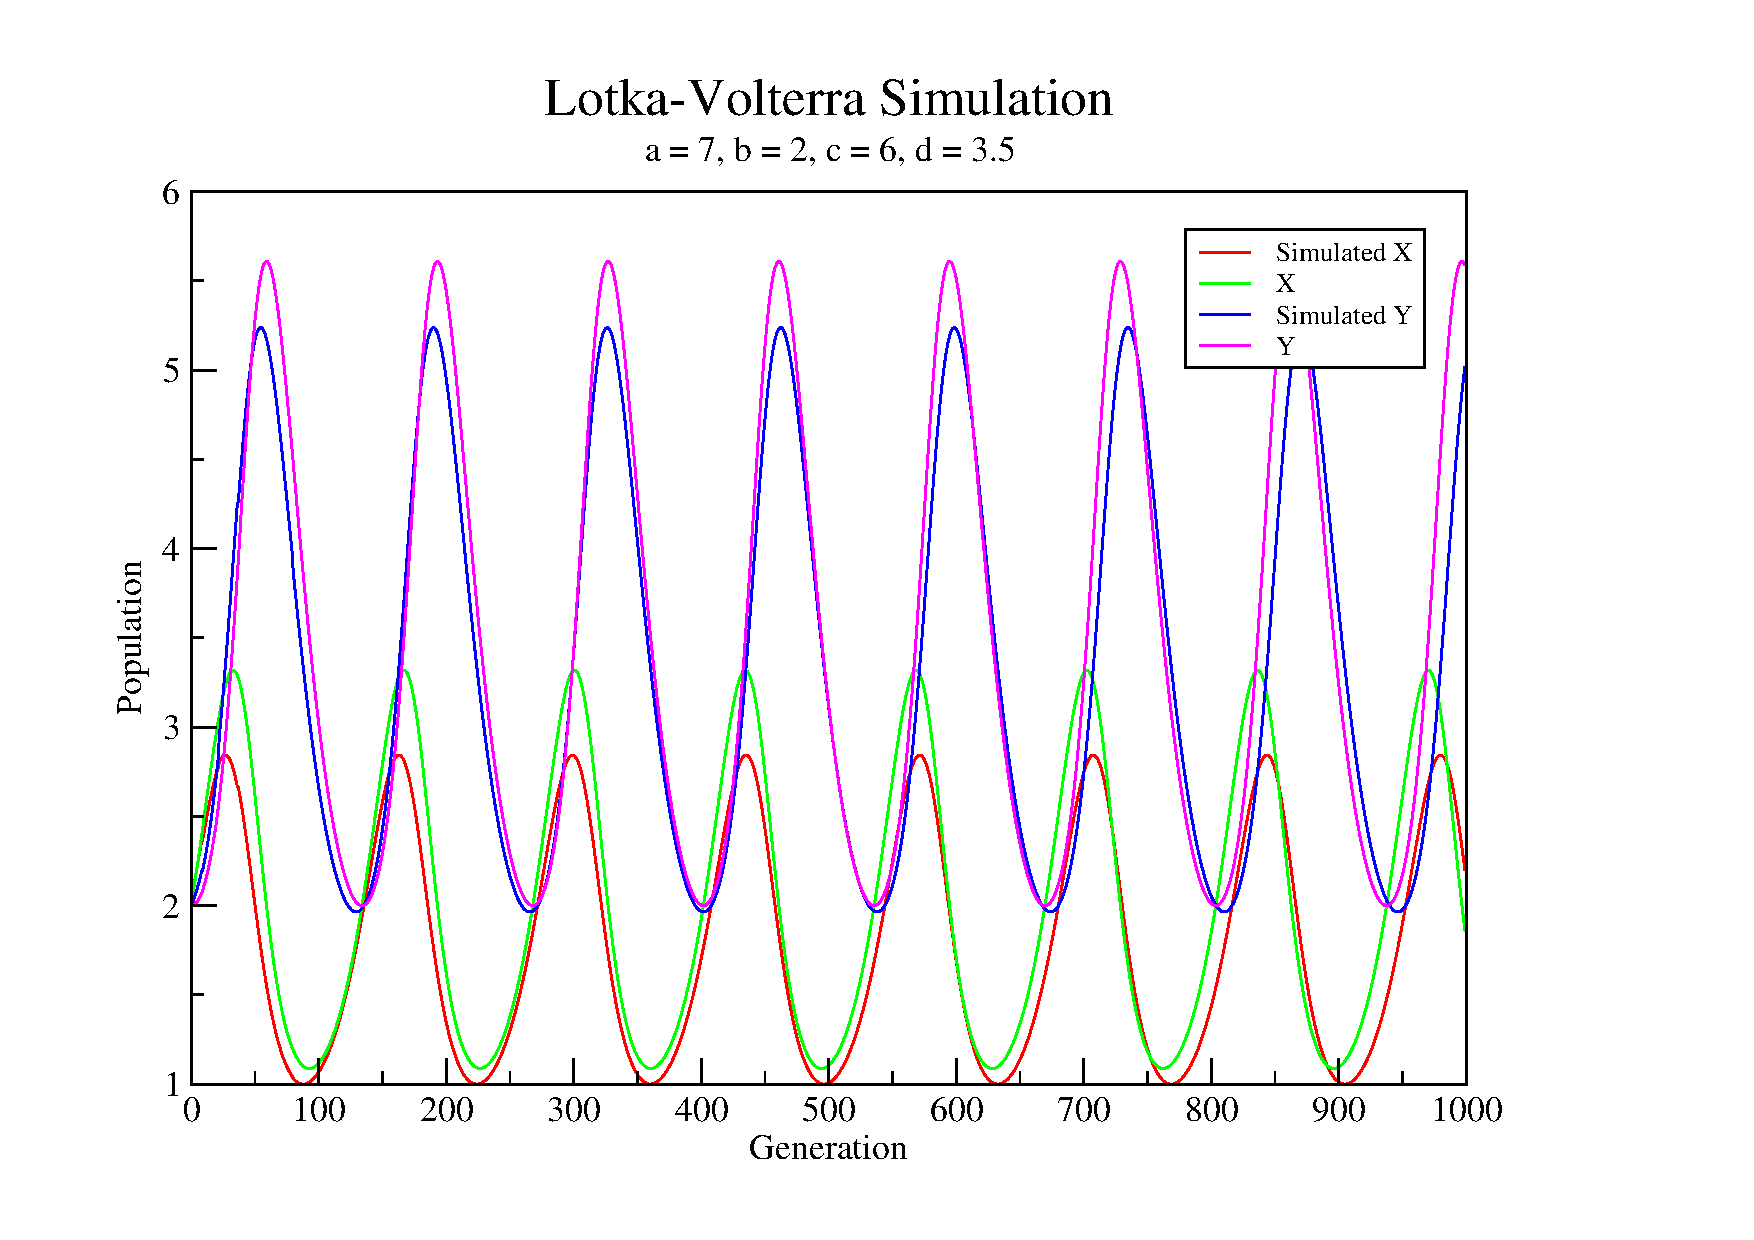
\includegraphics[width=13cm, trim=50px 35px 125px 30px, clip=true]{./03-parameterestimationmethodologies/data/LV_data.pdf}
 % Simulation.png: 800x600 pixel, 72dpi, 28.22x21.17 cm, bb=0 0 800 600
 \caption[{Simulation results of the Lotka-Volterra validation run.}]{{\bf Simulation results of the Lotka-Volterra validation run.}
 \label{fig:simulation}}
\end{figure}

\begin{figure}[tbp]
 \centering
 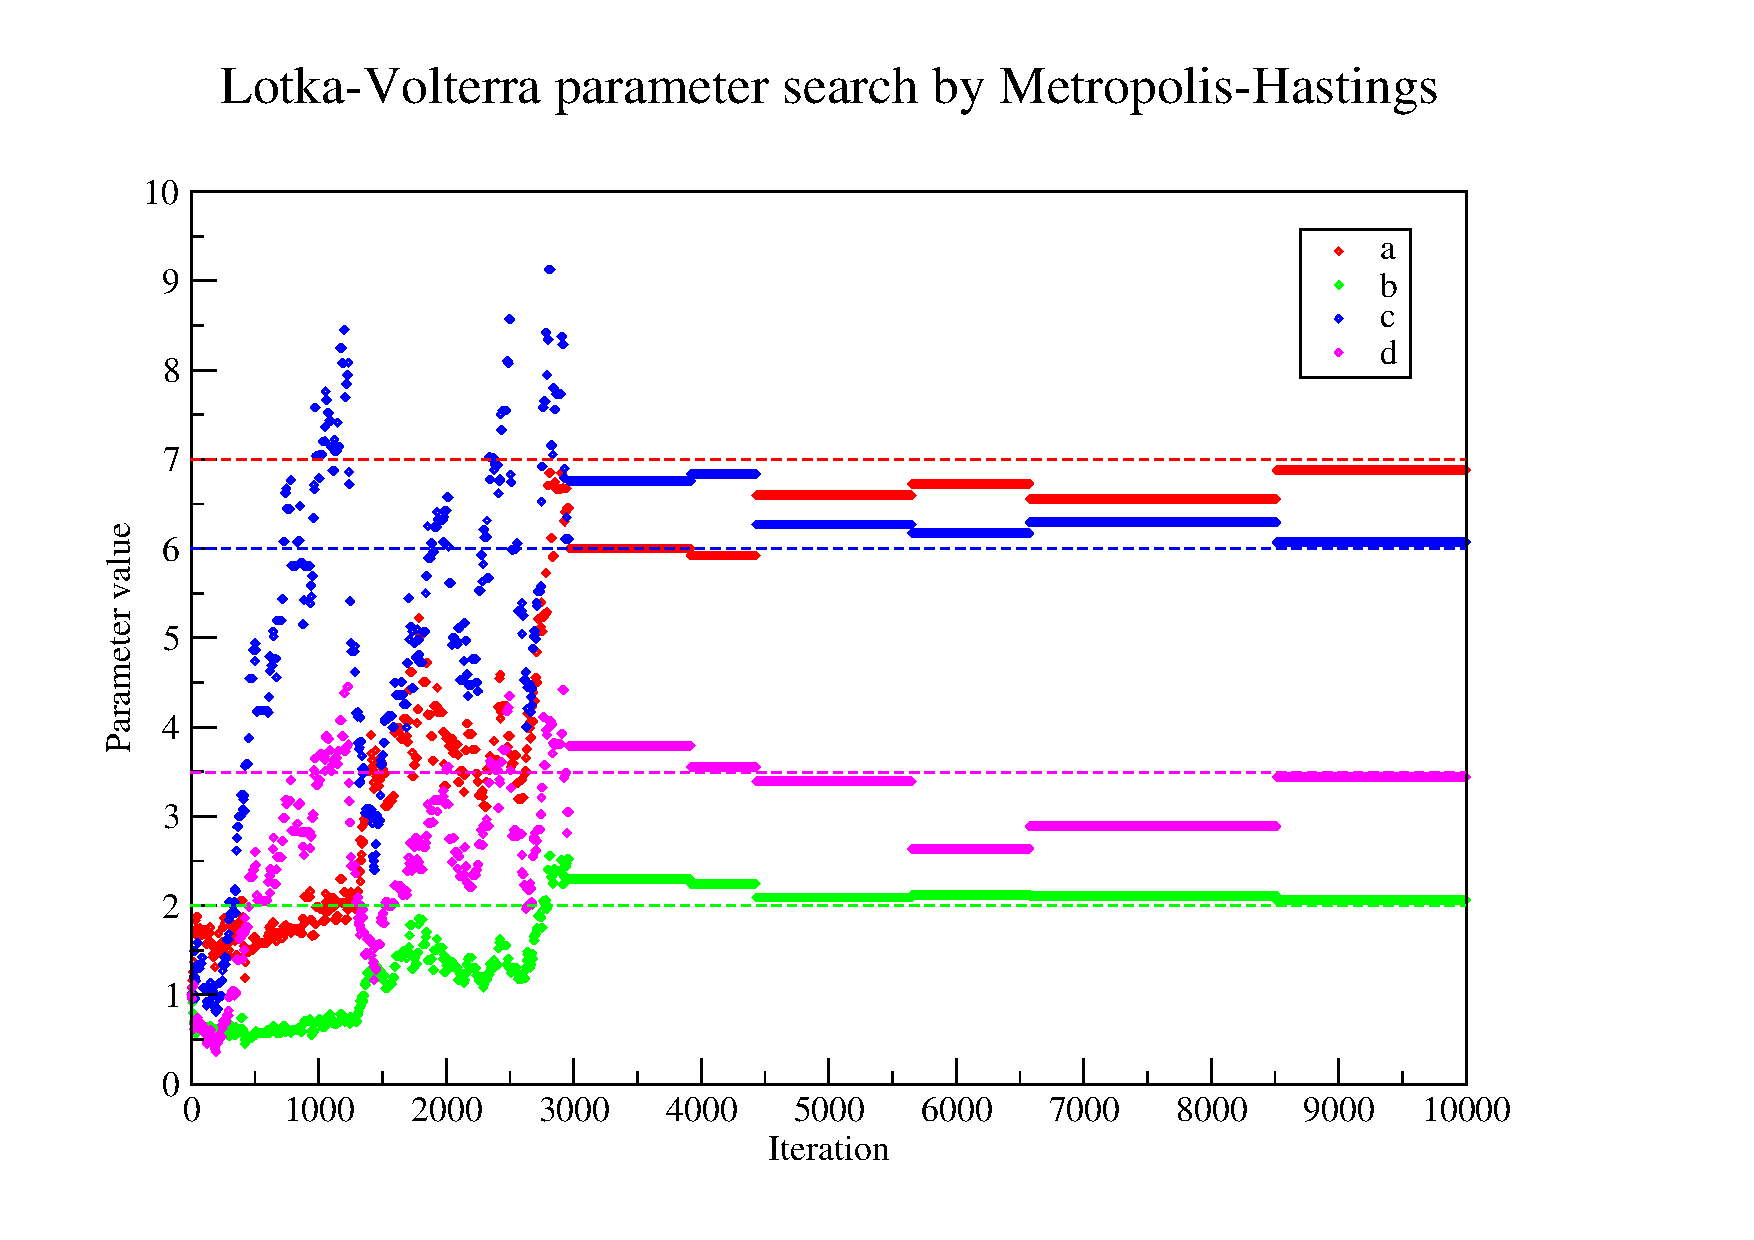
\includegraphics[width=13cm, trim=50px 35px 125px 30px, clip=true]{./03-parameterestimationmethodologies/data/LV_MCMC.pdf}
 % Simulation.png: 800x600 pixel, 72dpi, 28.22x21.17 cm, bb=0 0 800 600
 \caption[{MHMC results of the Lotka-Volterra validation run.}]{{\bf MHMC results of the Lotka-Volterra validation run.} Note the initial burn-in period followed by the distribution trajectory.
 \label{fig:parameters}}
\end{figure}
\afterpage{\clearpage}

\section{An Integrated Parameter Estimation Scheme Combining MHMC With Bayesian Inference}
In order to correctly parametrise the complex model being investigated it would have been impossible to use a MHMC-based parameter estimation algorithm alone, since it would be difficult to generate dataset which could provide enough information to estimate all the parameters at once. This being the case the parameter estimation algorithm was combined with a Bayesian approach to generating the proposal/prior distributions. Each run of MHMC will generate a Markov-Chain which can be used to calculate a posterior probability distribution for each parameter. These posterior probability distributions could be used to inform a subsequent round of parameter estimation in a Bayesian manner by using these distributions as the proposal/prior distributions for that subsequent round. This approach relies on the overall problem being able to be broken down into smaller problems which add increasing amounts of information. Thus the initial round of parameter estimation may only be estimating a small percentage of the total number of parameters, \textit{but} the posterior probability distributions generated can be used as informed prior probability distributions for a second round of parameter estimation which include more parameters. The entire scheme is represented visually in Figure \ref{fig:intscheme}.

\begin{sidewaysfigure}[tbp]
 \centering
 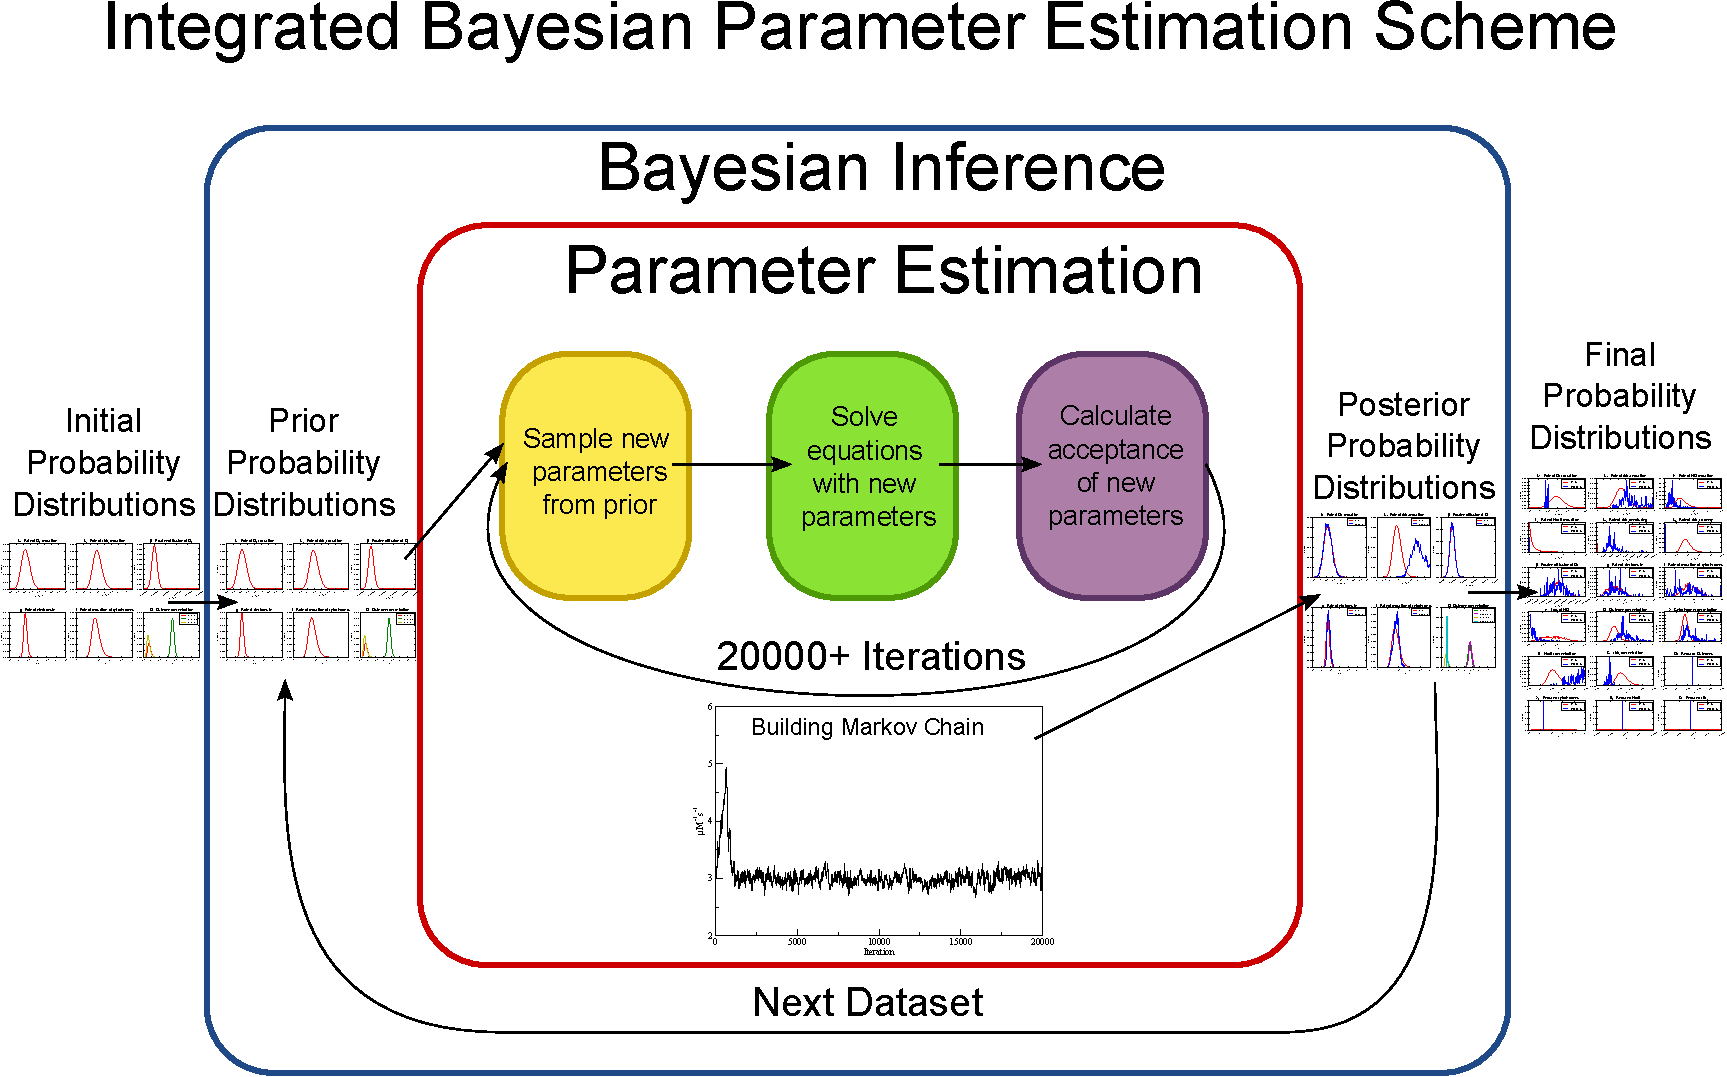
\includegraphics[width=20.4cm]{./03-parameterestimationmethodologies/data/paramest.pdf}
 \caption[{The Integrated Bayesian Parameter Estimation Scheme}]{{\bf The Integrated Bayesian Parameter Estimation Scheme.} This figure shows a flow-chart representing the major steps in the scheme. The initial probability distributions may be uniform, depending on how much knowledge is available \textit{a prioi}. The experimental data is compared to the solved data in the purple box. After sufficient iterations of parameter estimation, the Markov Chains are used to produce posterior probability distributions.
 \label{fig:intscheme}}
\end{sidewaysfigure}

\section{Implementing the Integrated Scheme}
As described previously, one dataset alone is not sufficient to provide enough information to be able to parametrise the model. In order to correctly perform Bayesian informed parameter estimation, the mathematical model needed to be separated into simpler units which could more easily be described by specific sets of experimental data. These simpler units would each provide information on a subset of the total number of parameters in the model.

The model was separated such that the simplest parts could be parametrised first. In this case, the simplest section of the model was those equations which describe oxygen respiration. This only requires one enzyme (although it does still require the electron transport chain). This section of the model also has the simplest experimental dataset.

These simplified datasets are parametrised, with each dataset analysed at least 10 times, generating at least 10 Markov Chains per parameter. These repeats are performed to provide statistical significance by reducing bias that could be introduced by using only 1 Markov Chain.

After this section of the model has been parametrised, posterior probability distributions are calculated, new sections are added and the process (shown in Figure \ref{fig:intscheme}) repeated, until all of the parameters have been estimated.

At this point the output probability distributions should be representative of the true parameter values for all the components in the model, subject to certain caveats such as the fact that parts of the model are simplified. These probability distributions should be accurate enough that they can be used to predict the behaviour of the biological system \textit{in vivo}.

%Experimental data was gathered for the first dataset, and this is used as a training set, with almost flat priors based on preliminary experimental data. The data was pre-processed and normalised if necessary and then presented to the Bayesian Parameter Estimation system. The MHMC algorithm samples from the prior distribution and then uses those samples as parameters to solve the model. It aims to improve the calculated likelihood and is ordinarily run for at least 10,000 iterations to give the system time to settle on the fittest parameters. The system is run on the same dataset 10 times to generate statistically significant results. The eventual output of the MHMC runs are posterior probability distributions for each of the parameters in the model. In accordance with Bayesian inference these are then used as prior distributions.

%At this point the next section of the model to be parametrised is decided, the appropriate experimental data identified and obtained, and the process is repeated until the entire model has been populated. The final result should be a set of reasonably narrow probability distributions for each of the parameters which describe the system accurately enough to correctly predict the behaviour of the system \textit{in vivo}.
\svnid{$Id$}
\chapter{Model - Construction and Parameters}
\label{chap:model}
\section{Construction}

The model was constructed based on existing knowledge of the respiratory chain in \Nsm{} from the ETC shown in Figure \ref{fig:etc} (Chapter \ref{chap:intro}). No \textit{a priori} assumptions are made about separation of time-scales that would permit the use of Michaelis-Menten kinetics, as the rates of intermediate reaction steps are not known. This approach also permits tracking of the oxidation state of all the intermediates which allows understanding and offers the potential for predictions that may be explored in future \textit{in vivo} studies.

The model was generated as a set of ordinary differential equations which describe the bulk-average concentration of substrates, products, enzymes and their activity within a well-mixed vessel. No assumptions are made about the bacterial population structure or the variations in concentrations of substrates between the bulk media and within the bacterial cells. Stochastic effects are ignored at the protein level, but they are unlikely to be of importance. Initially protein production is largely ignored as the switching mechanism is thought to happen on a time-scale that is much shorter than the transcription and translation of new proteins, they are therefore assumed to be expressed constitutively except where stated otherwise. However some datasets were available in the published literature\cite{Rock2005} that suggested otherwise, and were tested using an extension to the model described below which includes transcription and translation of certain components.

\subsection{Converting Biological Reactions into Differential Equations}
The rationale for obtaining the form for each of the 9 component equations is described below. Throughout the model the reduced components, i.e. those with available electrons, are denoted as active and have a subscript $a$. Components lacking a subscript denote the total, constant, amount of a component. $\emptyset$ denotes nothing (this is used as the source or sink when substrates are entering or exiting the system).

\subsubsection{Respiratory Substrates}
{\bf Oxygen}\\
The change in concentration of oxygen is affected by the following kinetic processes.
\begin{equation*}
\begin{gathered}
\emptyset\xrightarrow{\beta} O_2\\
O_2 + C_a\xrightarrow{k_1} H_{2}O + C_i
\end{gathered}
\end{equation*}
where $\beta$ is the rate of passive diffusion (as a function of \cOxygen{} concentration) of \cOxygen{} into the electrode chamber. The rate constant $k_1$ describes the reduction of oxygen and the oxygen reductase \cbbthree{}; this rate depends on the concentration of reduced (i.e. active) \cbbthree{}, $C_a$ and the concentration of $O_2$.
The differential equation that gives the change in oxygen concentration is
\begin{equation}
\frac{d[O_2]}{dt} = \beta(1-[O_2]/K_O) - k_{1}[C_a][O_2]
\label{eq:oxygen}
\end{equation}
In isolation the first term gives rise to a simple exponential input of oxygen until the saturation level ($K_O$) is reached. One small complication encountered was that $\beta$ is itself affected by the amount of bacteria in the vessel which has implications for fitting. Further details are given in Chapter \ref{chap:oxygenreduction}.\\ \\
%This is inversely proportional to oxygen concentration in the chamber, and limited to the oxygen saturation concentration, $K_O$. This component of the equation is required to account for a peculiarity of the experimental set-up, whereby the rate of diffusion of oxygen into the system depends on the density of the bacterial culture, and is not insignificant. $k_{1}$ is the rate of reduction of oxygen by the oxygen reductase \cbbthree{}. This rate depends on the concentration of reduced (i.e. active) \cbbthree{}, $C_a$ and the concentration of \cOxygen{}.%
{\bf Nitric Oxide}\\
The change in nitric oxide concentration is affected by the following kinetic processes.
\begin{equation*}
\begin{gathered}
NO_2^- + A_a \xrightarrow{m_1} NO + A_i\\
NO + B_a \xrightarrow{l_1} N_2O + B_i\\
NO + C_a \xrightarrow{k_5} NO\mhyphen C_X\\
NO\mhyphen C_X \xrightarrow{k_6} NO + C_a\\
NO \xrightarrow{\gamma} \emptyset
\end{gathered}
\end{equation*}
The equations above have a number of additional interactions in comparison to $\mathrm{O}_2$. NO is created by the reduction of $\mathrm{NO}_\mathrm{2}^\mathrm{-}$ by AniA, is reduced by its dedicated reductase, NorB, and converted to $\mathrm{N}_2\mathrm{O}$ which is lost from the cell, interacts with \cbbthree{}, and is also spontaneously lost from the electrode chamber. It is assumed that the interaction with \cbbthree{} occurs only in a reversible manner, leading to an NO bound and temporarily inactive form $C_X$. There is evidence that this interaction can also lead to permanent degradation of \cbbthree{} via the formation of peroxynitrite at the terminal oxidase. This is not currently considered in this version of the model. These effects are described mathematically in the equation below.
%The equation for describing \cNO{} concentration changes is more complex as \cNO{} has a number of additional interactions in comparison to \cOxygen{}. \cNO{} also interacts with \cbbthree{}, in addition to being reduced from \cNitrite{}, reduced to \cNtwoO{} and spontaneously lost from the electrode chamber. Currently this is the equation being used to model \cNO{} concentration.
\begin{equation}
\frac{d[NO]}{dt} = m_{1}[NO_2^-][A_a] - l_1[NO][B_a] - k_5[C_a][NO] + k_6 [C_X] - \gamma[NO]
\label{eq:no}
\end{equation}
The rate of synthesis of NO is captured by the first term, with rate constant $m_{1}$ and depends on the both the concentration of $\mathrm{NO}_\mathrm{2}^\mathrm{-}$ and reduced AniA ($A_a$). The reduction of NO is described by the next term with the rate constant $l_1$ and also depends on the concentration of NO and reduced NorB ($B_a$). Inhibition of \cbbthree{} by NO is modelled by the $\mathrm{3}^\mathrm{rd}$ component of the equation. $k_5$ is the rate constant describing the reversible binding of NO to \cbbthree{} to form the inactive form of \cbbthree{}, $C_X$. $k_6$ is the rate of recovery of this inhibited \cbbthree{}. $\gamma$ is the spontaneous rate of loss of NO from the electrode chamber.\\
%The synthesis of \cNO{} is modelled by $m_{1}$ which is the rate of \cNitrite{} reduction by reduced (active) AniA. This also depends on the concentration of \cNitrite{} and reduced AniA ($A_a$). The reduction of \cNO{} requires $l_1$ which is the rate of reduction of \cNO{} by reduced (active) NorB. This depends on the concentration of \cNO{} and reduced NorB ($B_a$). Inhibition of \cbbthree{} by \cNO{} is modelled by the \engordnumber{3} component of the equation. $k_5$ is the rate of inhibition of \cbbthree{} by \cNO{}. $k_6$ is the rate of recovery of inhibited \cbbthree{}. $\gamma$ is the rate of spontaneous loss of \cNO{} from the electrode chamber.
{\bf Nitrite}\\
The change in nitrite concentration is affected by the following kinetic process.
\begin{equation*}
NO_2^- + A_a \xrightarrow{m_1} NO + A_i
\end{equation*}
Which can be modelled mathematically by this equation
\begin{equation}
\frac{d[NO_2^-]}{dt} = - m_{1}[NO_2^-][A_a]
\label{eq:nitrite}
\end{equation}
where $m_{1}$ is the rate of reduction of \cNitrite{} by reduced (active) AniA ($A_a$).

\subsubsection{Electron Transporters}

In addition to the rate of change of concentration of the respiratory substrates, the model also contains information about the upstream state of components of the transfer chain, starting from the quinone pool. The ultimate upstream source of electrons into the respiratory chain is from NADH, but for the sake of simplicity all processes prior to the quinone pool are subsumed into a simple single rate. This simplification is made to avoid further complications associated with varying metabolism and to avoid distraction from the stated primary aim of understanding the switching behaviour of the downstream chain. The quinone pool was chosen as the starting point because it is known that NorB draws electrons directly from this point and therefore this represents the first branch in the chain. The desire was to understand how competition for electrons at branches affects function and therefore the quinone pool is included in the model.\\
%In addition to the rate of change of concentration of the respiratory substrates, the model also contains information about the state of the quinone pool, which is the upstream source of electrons into the respiratory chain. This is important because this affects the rate of reduction of the various enzymes which perform the substrate reductions. The equation for modelling the change in reduction state (activity) of the quinone pool is
{\bf Quinones}\\
The change in concentration of reduced quinones is affected by the following kinetic processes.
\begin{equation*}
\begin{gathered}
Q_i \xrightarrow{g} Q_a\\
B_i + Q_a \xrightarrow{l_3} B_a + Q_i\\
X_i + Q_a \xrightarrow{f} X_a + Q_i
\end{gathered}
\end{equation*}
The differential equation that models these reactions is
\begin{equation}
\frac{d[Q_a]}{dt} = g([Q] - [Q_a]) - l_3[Q_a]([B] - [B_a]) - f[Q_a]([X]-[X_a])
\label{eq:quinones}
\end{equation}
$Q_a$ is the reduced quinone, and $Q$ the total concentration of quinones in the system ($Q_i$ is calculated from these two values). $g$ represents the constant rate of availability of electrons into the quinone pool from NADH. The reduction of NorB by active quinones is parametrised by the rate constant $l_3$. NorB and reduced NorB are given by $B$ and $B_a$ respectively. As the quinones also reduce the cytochromes, this also needs to be modelled. $f$ is the rate constant parametrising the reduction of cytochromes by the active quinones. Total cytochromes and total reduced cytochromes are given by $X$ and $X_a$ respectively which are used to calculated $X_i$ in the kinetic process.\\
{\bf Cytochromes}\\
A simplified version of cytochromes was used and therefore $X$ actually represents a pool of different cytochromes, \textit{c$_{\textrm{x}}$}, \textit{c$_{\textrm{4}}$}, \textit{c$_{\textrm{5}}$} and the \textit{bc$_{\textrm{1}}$} complex. These are amalgamated into one here to simplify the equations and focus on the simple branching of the chain and competition for electrons. This is a modelling choice and it is further discussed in Chapter \ref{chap:completedmodel}.
%$Q_a$ is the reduced quinone, and $Q$ the total concentration of quinones in the system. $g$ represents the rate of flow of electrons into the quinone pool from NADH. The rate of reduction of NorB by active quinones is given by $l_3$. NorB and reduced NorB are given by $B$ and $B_a$ respectively. As the quinones also reduce the cytochromes, this also needs to be modelled. $f$ denotes the rate of reduction of cytochromes by the active quinones. Cytochromes and reduced cytochromes are given by $X$ and $E$ respectively.

%Given that the concentration of active cytochromes changes, due to reduction by the quinone pool and oxidation by the downstream enzymes, and this concentration is a parameter in (\ref{eq:quinones}), it also needs to be included in the model, and this is given by the following equation
The concentration of active cytochrome pool changes due to both reduction by the upstream quinone pool and oxidation by both of the remaining downstream terminal enzymes can be seen in the following kinetic processes.
\begin{equation*}
\begin{gathered}
C_i + X_a \xrightarrow{k_3} C_a + X_i\\
A_i + X_a \xrightarrow{m_3} A_a + X_i\\
X_i + Q_a \xrightarrow{f} X_a + Q_i
\end{gathered}
\end{equation*}
These are modelled with the following differential equation
\begin{equation}
\frac{d[X_a]}{dt} = -k_3([C] - [C_a] - [C_X])[X_a]  - m_3([A] - [A_a])[X_a] + f[Q_a]([X]-[X_a])
\label{eq:cytochromes}
\end{equation}
where $k_3$ is the rate constant describing the reduction of the available oxidised cytochrome c oxygen reductase (\cbbthree{}) by the quinone pool (via \textit{c$_{\textrm{x}}$} \& \textit{c$_{\textrm{4}}$}). $C$, $C_a$ and $C_X$ represent the overall concentration of \cbbthree{}, reduced (active) \cbbthree{} and NO inhibited \cbbthree{} respectively. $m_3$ is the rate constant describing the reduction of AniA by the cytochrome pool (via \textit{c$_{\textrm{5}}$}). The concentration of active cytochromes is thus increased by their reduction by the quinone pool, but this in turn can reduce the flux from the pool because less oxidised cytochrome is available to accept electrons. As stated previously, the relative time scales are unknown so all processes appear explicitly.
%where $k_3$ is the rate of reduction of the cytochrome c oxygen reductase (\cbbthree{}) by the quinone pool (via \textit{c$_{\textrm{x}}$} \& \textit{c$_{\textrm{4}}$}). $C$, $C_a$ and $C_X$ represent the overall concentration of \cbbthree{}, reduced (active) \cbbthree{} and NO inhibited \cbbthree{} respectively. $m_3$ is the rate of reduction of AniA by the cytochrome pool (via \textit{c$_{\textrm{5}}$}). The concentration of active cytochromes increases by their reduction by the quinone pool.

\subsubsection{Terminal Reductases}
Finally the changes in concentration of reduced terminal oxidases, \cbbthree{}, AniA and NorB are described by the following equations. All the terms present in this section have been introduced previously. These equations of course could equally have been written for the oxidised form but these can easily be recovered because it is assumed that the total concentration of the oxidases remains constant.\\
%To model the changes in concentration of the individual enzymes, \cbbthree{}, AniA and NorB, the following equations are used:
{\bf Reduced \cbbthree{}}\\
The kinetic processes which affect the concentration of reduced (active) \cbbthree{} are
\begin{equation*}
\begin{gathered}
C_i + X_a \xrightarrow{k_3} C_a + X_i\\
O_2 + C_a\xrightarrow{k_1} H_{2}O + C_i\\
NO + C_a \xrightarrow{k_5} NO\mhyphen C_X\\
NO\mhyphen C_X \xrightarrow{k_5} NO + C_a
\end{gathered}
\end{equation*}
which is described by
\begin{equation}
\frac{d[C_a]}{dt} = k_3([C] - [C_a] - [C_X])[X_a] - k_{1}[C_a][O_2] - k_5[C_a][NO] + k_6[C_X]
\label{eq:active_cbb3}
\end{equation}
\\
{\bf Inhibited \cbbthree{}}\\
The following kinetic process alters the concentrations of reversibly inhibited \cbbthree{}.
\begin{equation*}
\begin{gathered}
 NO + C_a \xrightarrow{k_5} NO\mhyphen C_X \xrightarrow{k_6} NO + C_a
\end{gathered}
\end{equation*}
which is described by
\begin{equation}
\frac{d[C_X]}{dt} = k_5[C_a][NO] - k_6 [C_X]
\label{eq:NO inhibited_cbb3}
\end{equation}
\\
{\bf Reduced AniA}\\
The concentration of reduced AniA is affected by the following kinetic processes.
\begin{equation*}
\begin{gathered}
A_i + X_a \xrightarrow{m_3} A_a + X_i \\
NO_2^- + A_a \xrightarrow{m_1} NO + A_i 
\end{gathered}
\end{equation*}
which can be modelled by
\begin{equation}
\frac{d[A_a]}{dt} = m_3([A] - [A_a])[X_a]- m_{1}[NO_2^-][A_a]
\label{eq:active_ania}
\end{equation}
\\{\bf Reduced NorB}\\
Changes in NorB concentration occur via the following kinetic processes.
\begin{equation*}
\begin{gathered}
B_i + Q_a \xrightarrow{l_3} Q_i + B_a \\
NO + B_a \xrightarrow{l_1} N_{2}O + B_i
\end{gathered}
\end{equation*}
and are modelled by this equation
\begin{equation}
\frac{d[B_a]}{dt} = l_3[Q_a]([B] - [B_a]) - l_1[NO][B_a]\\
\label{eq:active_norb}
\end{equation}


\subsection{Assumptions and their Justifications}
A number of assumptions were made regarding the kinetics and reactions taking place in the model.
\begin{enumerate}
 \item {\bf It is assumed that NO inhibits the reduced \cbbthree{} and not the oxidised form, since it is not expected that Nitric oxide to bind to an inactive enzyme.} This is corroborated by \citet{Giuffre2000}, who show significant levels of inhibition of reduced cytochrome. They do also however observe low levels of inhibition of the oxidised enzyme also. Their experiments used cytochrome c oxidase (aa3) rather than \cbbthree{}, but I believe this assumption still stands as the enzymes are of the same family. This also implies that the model deals exlusively with reversible inhibition.
 \item {\bf Bacterial population structure and concentration variation not considered.} The primary substrates of interest are gases and substrates which are thought to freely diffuse in and out of the cells. Additionally the culture is kept well-mixed at all times, thus it can be assumed that the culture is homogenous.
 \item {\bf No backwards reactions.} For simplicity, backwards reactions are not included. However they may be important, and could easily be included in a future study with the concommitant increase in parameter count.
 \item {\bf No Michaelis-Menten kinetics.} Separation of time-scales cannot be assumed as the rates of intermediate reaction steps are not known. Future information regarding timescale separation could easily be incorporated.
 \item {\bf All cytochromes can be modelled as one.} The main effort of modelling was to concentrate on the position of branches in the respiratory chain. In the same way the effects of Laz and $c_5$ on AniA and \cbbthree{} respectively can also be ignored. They are not the prime electron donors to their terminal reductases and contribute very little overall to the reduction\cite{Deeudom2007}.
\end{enumerate}

%Also, values are in the right ball park even though they are using aa3 rather than \cbbthree. $10^8 M ^{-1} s ^{-1}$ against around $50 \mu M ^{-1} s ^{-1}$.

\section{Parameters and their Prior Distributions}

None of the rate constants or concentrations which were required for this model have previously been determined for \Nsm, so values from other similar organisms had to be used instead. In some cases there appears to be no data in the literature regarding values of particular components. Table \ref{tab:ps} lists the values that have been obtained from the literature.

\begin{table}[tbp]
\begin{center}
\begin{tabular}{>{\centering}m{1.7cm}>{\centering}m{6.2cm}>{\centering}m{2.5cm}>{\centering}m{2.8cm}}
\toprule
\textbf{Symbol} & \textbf{Description} & \textbf{Value} & \textbf{Source}
\tabularnewline
\midrule
$k_1$ & Rate of O$_{\textrm{2}}$ reduction by reduced \cbbthree{} & $415~\mu M^{-1} s^{-1}$ & \citet{Forte2001} and \citet{Hunter2007}
\tabularnewline\noalign{\smallskip}\hline\noalign{\smallskip}

$k_3$ & Rate of \cbbthree{} reduction by cytochrome pool & $3~\mu M^{-1} s^{-1}$ & \citet{Chang2010}
\tabularnewline\noalign{\smallskip}\hline\noalign{\smallskip}

$l_1$ & Rate of NO reduction by reduced NorB & Unknown & N/A
\tabularnewline\noalign{\smallskip}\hline\noalign{\smallskip}

$l_3$ & Rate of NorB reduction by quinone pool & Unknown & N/A
\tabularnewline\noalign{\smallskip}\hline\noalign{\smallskip}

$m_1$ & Rate of NO$_{\textrm{2}}^{\textrm{-}}$ reduction by reduced AniA & Unknown & N/A
\tabularnewline\noalign{\smallskip}\hline\noalign{\smallskip}

$m_3$ & Rate of AniA reduction by cytochrome pool & $4.8\pm0.2~\mu M^{-1}s^{-1}$ & \citet{Nojiri2009}
\tabularnewline\noalign{\smallskip}\hline\noalign{\smallskip}

$k_5$ & Rate of \cbbthree{} inhibition by NO & $100~\mu M ^{-1} s ^{-1}$ & \citet{Giuffre2000} and \citet{Blackmore1991}
\tabularnewline\noalign{\smallskip}\hline\noalign{\smallskip}

$k_6$ & Rate of recovery of NO inhibited \cbbthree{} & Unknown & N/A
\tabularnewline\noalign{\smallskip}\hline\noalign{\smallskip}

$\beta$ & Rate of passive diffusion in of O$_{\textrm{2}}$ & Unknown & N/A
\tabularnewline\noalign{\smallskip}\hline\noalign{\smallskip}

$K_O$ & Saturation O$_{\textrm{2}}$ level & $48~\mu M$ & This work
\tabularnewline\noalign{\smallskip}\hline\noalign{\smallskip}

$g$ & Rate of electrons in from NADH & $0.8~s^{-1}$ & This work
\tabularnewline\noalign{\smallskip}\hline\noalign{\smallskip}

$f$ & Rate of reduction of cytochromes by quinones & $8~\mu M^{-1}s^{-1}$ & This work
\tabularnewline\noalign{\smallskip}\hline\noalign{\smallskip}

$\gamma$ & Spontaneous loss of NO & Unknown & N/A
\tabularnewline\noalign{\smallskip}\hline\noalign{\smallskip}

$Q$ & Concentration of quinones & $0.3~\mu M$ & \citet{Hedrick1986}
\tabularnewline\noalign{\smallskip}\hline\noalign{\smallskip}

$X$ & Concentration of cytochromes & $\approx3.97~\mu M$ & \citet{Deeudom2007}
\tabularnewline\noalign{\smallskip}\hline\noalign{\smallskip}

$A$ & Concentration of AniA & $0.003 - 0.03~\mu M$ & This work
\tabularnewline\noalign{\smallskip}\hline\noalign{\smallskip}

$B$ & Concentration of NorB & $0.003 - 0.03~\mu M$ & This work
\tabularnewline\noalign{\smallskip}\hline\noalign{\smallskip}

$C$ & Concentration of \cbbthree{} & $0.003 - 0.03~\mu M$ & This work
\tabularnewline
\bottomrule
\end{tabular}
\caption[Model parameters]{{\bf Model parameters.} This table shows all the parameter values that have been obtained from the extant literature, or interpolated from preliminary experiments done during the course of this work. These values represent the initial data that is used to populate the model, from which all subsequent parameter sets are generated. For values that show concentrations of components, they represent the value for a culture with $OD_{600}=1.00$.
\label{tab:ps}}
\end{center}
\end{table}

\subsection*{Variables}
\subsubsection*{$\mathbf{O_2}$ {\bf- Oxygen concentration}}
This variable is always obtained directly from the experimental dataset as it indicates the starting point for oxygen in the model. It is calculated from a linear regression analysis of the first section of oxygen reduction to eliminate noise in the data.

\subsubsection*{$\mathbf{NO}$ {\bf- Nitric oxide concentration}, and $\mathbf{NO_2^-}$ {\bf- Nitrite concentration}}
As for Oxygen concentration, these variable is simply obtained from the dataset and the same conditions apply.

\subsubsection*{$\mathbf{X_a}$, $\mathbf{A_a}$, $\mathbf{B_a}$, $\mathbf{C_a}$, $\mathbf{Q_a}$ - Reduced enzyme concentrations, and $\mathbf{C_X}$ {\bf- Reversibly NO inhibited \cbbthree{}}}
These values are unknown at start of simulations. They have to be lower than the total concentrations for each enzyme, and the model enforces this. Given the rates of reduction of these enzymes they are all set to very low values, determined from exploratory runs of the parameter estimation algorithm. The rates of reduction for these enzymes actually make the initial value (so long as it is low) largely irrelevant as they reach their steady-state after only a few integration cycles.

\subsection*{Parameters}
\subsubsection*{$\mathbf{k_1}$ {\bf- Rate of O$_{\textrm{2}}$ reduction by reduced \cbbthree{}}}
%\citet{Preisig1996} show that \textit{B. japonicum} \cbbthree{} (\textit{fixNOQP}) has a $K_m$ of $55.7 \pm 24.2$ nM $\mathrm{O}_2$, and $V_{max}$ $37.4 \pm 9.2$ $\mathrm{nmol O}_2 \mathrm{min}^{-1} \mathrm{mg}^{-1}$.\\
%Given $v = \frac{V_{max}[S]}{K_m+[S]}$
%Then at high $O_2$ rate is:
%$v = \frac{37.4\times 100,000}{55.7+100,000} = 37.4~nmol^{-1}min{-1}mg{-1} = 0.000622986~\mu mol^{-1}s{-1}mg{-1}$\\

A value for $k_1$, the rate of O$_{\textrm{2}}$ reduction by reduced \cbbthree{} was calculated by using the $\mathrm{K}_{cat}$ value from \textit{Pseudomonas stutzeri}, and the $\textrm{k}_m$ value from \textit{Neisseria lactamica}, which \citet{Forte2001} and \citet{Hunter2007} determine are $166s^{-1}$ and $0.4\mu M$ respectively. $k_1$ can be calculated as $\frac{166s^{-1}}{0.4\mu M} = 415\mu M^{-1} s^{-1}$.

\subsubsection*{$\mathbf{k_3}$ {\bf- Rate of \cbbthree{} reduction by cytochrome pool}}
$k_3$, the rate of reduction of \cbbthree{} by the cytochromes was calculated from values obtained from the maximum reduction rate of \cbbthree{} by cytochrome $c_4$ in \textit{Vibrio cholerae} by \citet{Chang2010}. A rate of 300 electrons transported per second was observed with a cytochrome $c_4$ concentration of $100\mu M$. This concentration was not saturating, but there appears to be a linear relationship between rate and concentration. We assume that 1 electron equals 1 reduction of \cbbthree{}, thus the rate of reduction of \cbbthree{} by cytochromes is $\frac{300s^{-1}}{100\mu M} = 3\mu M^{-1} s^{-1}$.

\subsubsection*{$\mathbf{l_1}$ {\bf- Rate of NO reduction by reduced NorB}}
%240 and 256 nanomoles NO reduced per minute per OD600 unit as determined by \citet{Barth2009}.

An estimate for the rate of NO reduction by reduced NorB can be obtain from \citet{Rock2007}. They observed rates of NO reduction of $54 \pm 6~\mathrm{nmol min}^{-1} \mathrm{mg}^{-1}$. This was in total protein content from dry weight. Thus the rate of NO reduction is $0.9 \pm 0.1~\mu\mathrm{mol s}^{-1}\mathrm{g}^{-1}$ bacterial protein. The protein content of the cells was assumed to be similar to that of \textit{E. coli} at 50\% of dry weight, where each cell weighed 2pg. A culture of \textit{Neisseria meningitidis} with $OD_{600} = 1$ has $1 \times 10^9~\textrm{cells/ml}$, therefore the rate is $4.5~nmols^{-1}$ of quinones in 5ml culture ($5\times 10^9 \textrm{cells} \times 2\times 10^{-12}~\textrm{g} \times 50\% \times 0.9~\mu\mathrm{mol s}^{-1}\mathrm{g}^{-1}$), converted to molarity is $0.9~\mu Ms^{-1}$.

\subsubsection*{$\mathbf{l_3}$ {\bf- Rate of NorB reduction by quinone pool}}
No information available in the literature, so the rate is set to $1~\mu M^{-1}s^{-1}$.

\subsubsection*{$\mathbf{m_1}$ {\bf- Rate of NO$_{\textrm{2}}^{\textrm{-}}$ reduction by reduced AniA}}


\subsubsection*{$\mathbf{m_3}$ {\bf- Rate of AniA reduction by cytochrome pool}}
The value for $m_3$, the rate of reduction of AniA by cytochromes, is the observed electron transfer rate between the equivalent cytochrome and nitrite reductase from \textit{Achromobacter xylosoxidans}. A value of $4.8\pm0.2 \mu M^{-1}s^{-1}$ was observed during stopped-flow experiments by \citet{Nojiri2009}.

\subsubsection*{$\mathbf{k_5}$ {\bf- Rate of \cbbthree{} inhibition by NO}}
\citet{Giuffre2000} and \citet{Blackmore1991} showed with cytochrome \textit{c} oxidase that NO could bind reversibly and inhibit the activity of the enzyme. The rate they calculated was $10^8~M ^{-1} s ^{-1}$. I assume that even though the enzyme is different, its NO binding characteristics would be similar to that of \cbbthree{} as it is of the same family.

\subsubsection*{$\mathbf{k_6}$ {\bf- Rate of recovery of NO inhibited \cbbthree{}}}
\citet{Giuffre2000} calculated a half-life of t\textonehalf $\approx 80~\mathrm{min}$.\\
The apparent $K_d$ from \citet{Rock2007} was calculated to be about 500 nM, which tallies with values from $k_5$ and $k_6$.

\subsubsection*{$\beta$ {\bf- Rate of passive diffusion in of O$_{\textrm{2}}$}}
This value is highly dependent on the culture, and is in some way tied to the density of the culture, however the relationship is not known. During early experiments I noticed that oxygen diffusion was slower in high density cultures compared to those of low density, experiments to examine the relationship proved fruitless in determining any relationship. In addition this parameter is a product of the experimental set-up rather than the model itself.

\subsubsection*{$\mathbf{K_O}$ {\bf- Saturation O$_{\textrm{2}}$ level}}
This value is dependent on the particular culture being modelled, however its prior value is usually set to $48~\mu M$ as this figure was observed during experiments to determine oxygen diffusion rates into the culture.

\subsubsection*{$\mathbf{g}$ {\bf- Rate of electrons in from NADH (or rate of reduction of quinones)}}
This value is unknown, but initial runs of the algorithm suggest the value to be about $0.8~s^{-1}$.

\subsubsection*{$\mathbf{f}$ {\bf- Rate of reduction of cytochromes by quinones}}
\citet{Snyder2000} showed by reducing yeast cytochrome $\mathrm{bc}_1$ by using $25~\mu\mathrm{M}$ menaquinol the rate constants were $7.9~\mathrm{s}^{-1}$ for cytochrome b, and $1.55-6.9\times10^5~\mathrm{M}^{-1}\mathrm{s}^{-1}$ for cytochrome $\mathrm{c}_1$ (second order). However preliminary tests showed that a value of $8~\mu M^{-1}s^{-1}$ was more appropriate.

\subsubsection*{$\gamma$ {\bf- Spontaneous loss of NO}}
This value is assumed to be the same as the $\beta$, the rate of oxygen diffusion in across the liquid-gas barrier, as this is simply the reverse.


\subsubsection*{$\mathbf{Q}$ {\bf- Concentration of quinones}}
$Q$, the concentration of quinones was calculated based on data from \citet{Hedrick1986}. The protein content of the cells was assumed to be similar to that of \textit{E. coli} at 15\% of wet weight, where each cell weighed 2pg, and that there were $1\mu \textrm{mol}$ of respiratory quinones per g of bacterial protein. A culture of \textit{Neisseria meningitidis} with $OD_{600} = 1$ has $1 \times 10^9 \textrm{cells/ml}$, therefore there are 1.5nmol of quinones in 5ml culture ($5\times 10^9 \textrm{cells} \times 2\times 10^{-12} \textrm{g} \times 15\% \times 1\mu\textrm{mol/g}$), converted to molarity is $0.3\mu M$.

\subsubsection*{$\mathbf{X}$ {\bf- Concentration of cytochromes}}
\citet{Deeudom2007} suggests that the total cytochrome concentration (inc. \cbbthree{}) is about $4~\mu M$ in \Nsm{}. Thus subtracting the value for C leaves a concentration of $\approx 3.97~\mu M$.

\subsubsection*{$\mathbf{A}$, $\mathbf{B}$, $\mathbf{C}$ {\bf- Concentration of Respiratory enzymes}}
Given the lack of concrete values for these parameters, the assumption is that all the respiratory enzymes are present in roughly equal quantities. Based on the values given for Q above, there are $1.5~mg$ of cell protein in 5 ml of $OD_{600}=1$ culture. \cbbthree{} is thought to be about 0.1-1\% of the total cell protein
%10\% of cell is membrane.
and is approximately 100 kDa in molecular weight. Therefore converting these values to molarity gives a concentration of approximately 3-30 nM.

\section{Implementation of the model}
%By keeping the quantities involved in their original state and not making any assumption about time-scale separation I am able to make predictions regarding the transient oxidation states of the various components. These are potentially experimentally accessible and appear to be crucial for the dynamic response of the chain in different environments.

The model contains no implied information about cell density. This means the values for various component concentrations will differ between experiments. 
Initially the optical density of cultures was used to determine the cell density however experiments proved that this was not a completely reliable proxy for cell density as this also includes dead cells. Using optical density as a cell density proxy should give linear relationships between cell densities and reaction rates, however this proved not to be the case, with rates of oxygen reduction differing between cultures with the same optical density (data not shown). Therefore where possible, any normalisation that was carried out used the initial oxygen reduction rate as a relative indicator of living cells.

%The model contains no implied information about cell density. This means the values for various component concentrations will differ between experiments. Initially the optical density of cultures was used to determine the cell density however experiments proved that this was not a completely reliable proxy for cell density as this also includes dead cells. Using optical density as a cell density proxy should haven given linear relations between cell densities and reaction rates, however this proved not to be the case, with rates of oxygen reduction different between cultures with the same optical density. Therefore where possible, any normalisation that was carried out used the initial oxygen reduction rate as a relative indicator.

\section{Solving Ordinary Differential Equations}
The model equations (given previously) are solved in parallel using the common $\mathrm{6}^\mathrm{th}$ order Runge-Kutta-Fehlberg algorithm for integrating ordinary differential equations\cite{Butcher2003}. Adaptive step-sizes were implemented using the Cash-Karp method\cite{Cash1990}. The adaptive step size system was required as it prevented the introduction of systemic numerical instabilities (see appendix for further details of why this was necessary).

The parameter estimation system and ODE solver were a bespoke implementation written in Java. The Runge-Kutta algorithm was modified from that found in Numerical Recipes in C\cite{Press1992}. I decided to write a custom implementation rather than using off the shelf systems for solving ODEs and parameter estimation as I wanted the greatest flexibility in how I integrated the two techniques, and it allowed me to quickly and easily tailor the code to my needs. Initially I tried using COPASI \cite{Hoops2006}, however at that time it had limitations that I could not overcome, such as an inability to allow bulk addition of components at arbitrary time-points.

The implementation of the model has no constraints on respiratory substrate concentration, thus allows the altering of these concentrations whilst solving the equations. % however changes to substrate concentration have to be made programmatically to inform the model of the change (\texttt{if (t == 50) then NO\_conc += 20;}).
This ability means that the switch between aerobic and anaerobic respiration can be examined synthetically, and the model is also capable of simulating how the respiratory system responds to the sudden addition of substrates such as Nitric Oxide. More complicated methods are possible, but given the high diffusion of the substrates concerned as well as the deliberate injection of the relevant substrate this method was a simpler and reasonable mimic for my empirical method. This ability was an absolute requirement, as in order to fully parametrise the model it was necessary to isolate sections of the model, which required adding aliquots of respiratory substrate during respiration.

%This ability means that the switch between aerobic and anaerobic respiration can be examined synthetically, and the model is also capable of simulating how the respiratory system responds to addition of substrates such as Nitric Oxide. This ability was an absolute requirement, as in order to fully parametrise the model it was necessary to isolate sections of the model, which required adding aliquots of respiratory substrate during respiration.

\section{Parameter Estimation}
Estimating the parameter values for the components in the mathematical model involved comparing the biological results with those produced by solving the ODEs and adjusting the parameter values to minimise the difference between the two results. The different methods for parameter estimation that I investigated are detailed in Chapter \ref{chap:paramest} [\nameref{chap:paramest}].
\svnid{$Id$}
\chapter{Oxygen Reduction in \Nm{}}
\label{chap:oxygenreduction}
\section{Aerobic Reduction of Oxygen}
\subsection{Introduction}
The first dataset used in the iterative approach to parameter estimation was of a simple oxygen reduction experiment carried out in aerobic conditions. This dataset is the simplest biologically as under aerobic conditions and without the presence of any microaerobic substrates (nitrite or nitric oxide) the only respiratory pathway that is active is the oxygen reducing one. Additionally, the other parts of a respiratory chain influence the oxygen reducing pathway either by competing for electrons, or chemically inhibiting it. The relevant portions of the ETC are shown graphically in Figure \ref{fig:o2_resp_chain}.

\begin{figure}[tbp]
	\centering
	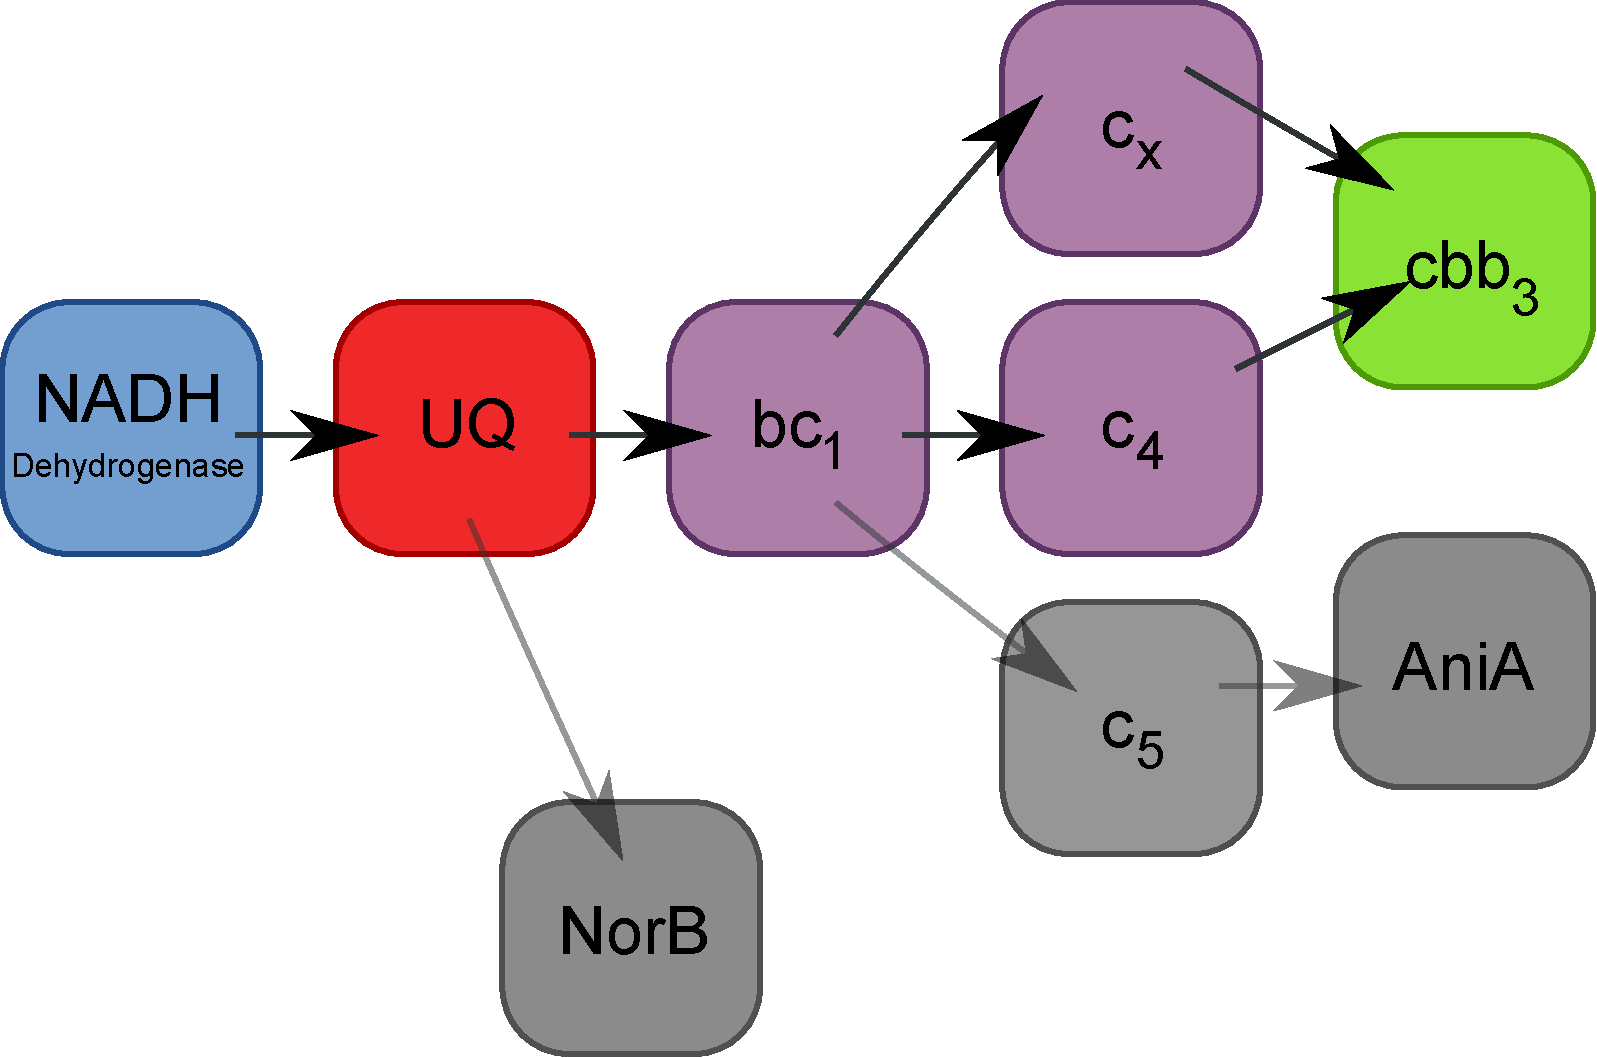
\includegraphics[width=14cm]{05-oxygenreduction/data/o2_resp_chain.pdf}
	\caption[Oxygen reducing electron transport chain of \Nm{}]{{\bf Oxygen reducing electron transport chain of \Nm{}.} This shows the complete electron transport chain of \Nsm{} with the components irrelevant to oxygen reduction greyed out. In the mathematical model all of the purple elements (cytochromes) are amalgamated into one entity.
	\label{fig:o2_resp_chain}}
\end{figure}

The equations that describe this portion of the ETC are:
\begin{eqnarray*}
\frac{d[O_2]}{dt} & = & \beta(1-[O_2]/K_O) - k_{1}[C_a][O_2]\\
\frac{d[Q_a]}{dt} & = & g([Q] - [Q_a]) - l_3[Q_a]([B] - [B_a]) - f[Q_a]([X]-[X_a])\\
\frac{d[X_a]}{dt} & = & -k_3([C] - [C_a] - [C_X])[X_a]  - m_3([A] - [A_a])[X_a] + f[Q_a]([X]-[X_a])\\
\frac{d[C_a]}{dt} & = & k_3([C] - [C_a] - [C_X])[X_a] - k_{1}[C_a][O_2] - k_5[C_a][NO] + k_6[C_X]
\end{eqnarray*}
These equations describe the change in concentration of oxygen over time, which is the experimentally observable value, the reduction state of the quinone pool and the reduction state of the cytochrome ``pool''. This portion of the model involved 13 parameters and variables which were to be estimated (the model actually contains 17 such parameters and variables, but under these conditions the remaining 4 are set to 0 as they are related to nitrite reduction effects). This large number of parameters will clearly result in over-fitting, however this was necessary to generate loose bounds for all of the parameters.

\subsection{Experimental Results}
Generation of oxygen reduction datasets required the growth of MC58 (wild-type \Nsm{}) in aerobic conditions until mid log-phase growth had been achieved. This corresponds to an $\mathrm{OD}_{600}$ of 0.3-0.9 and usually required an incubation period of roughly 3 hours. Once the required cell density had been obtained, the  culture was transferred to the oxygen electrode chamber and recorded the oxygen concentration as the culture respired. At this point the cells are only using whatever amount of oxygen is presently dissolved in the culture medium in addition to that diffusing in through the cap (negligible). Once the culture had used up all its dissolved oxygen, the electrode chamber cap was removed and the culture media aerated using a Pasteur pipette. This restores oxygen levels throughout the culture and allows the bacteria to continue respiring in aerobic conditions. A typical oxygen reduction plot is shown in Figure \ref{fig:oxy_repeatable_chl}. This is split into individual reduction sections, which can then be used as input data for parameter estimation. In many cases if the culture is allowed to become completely anaerobic for a prolonged period of time, the bacteria will die, evidenced by a subsequent lack of oxygen reduction, however this is not always the case as shown in Figure \ref{fig:repeat_oxy_with_delay}.

The experiments used to generate data for oxygen reduction are highly repeatable and consistently generate the same basic result of a linear reduction of oxygen with time.
\begin{figure}[p]
 \centering
 %trim = l b r t
 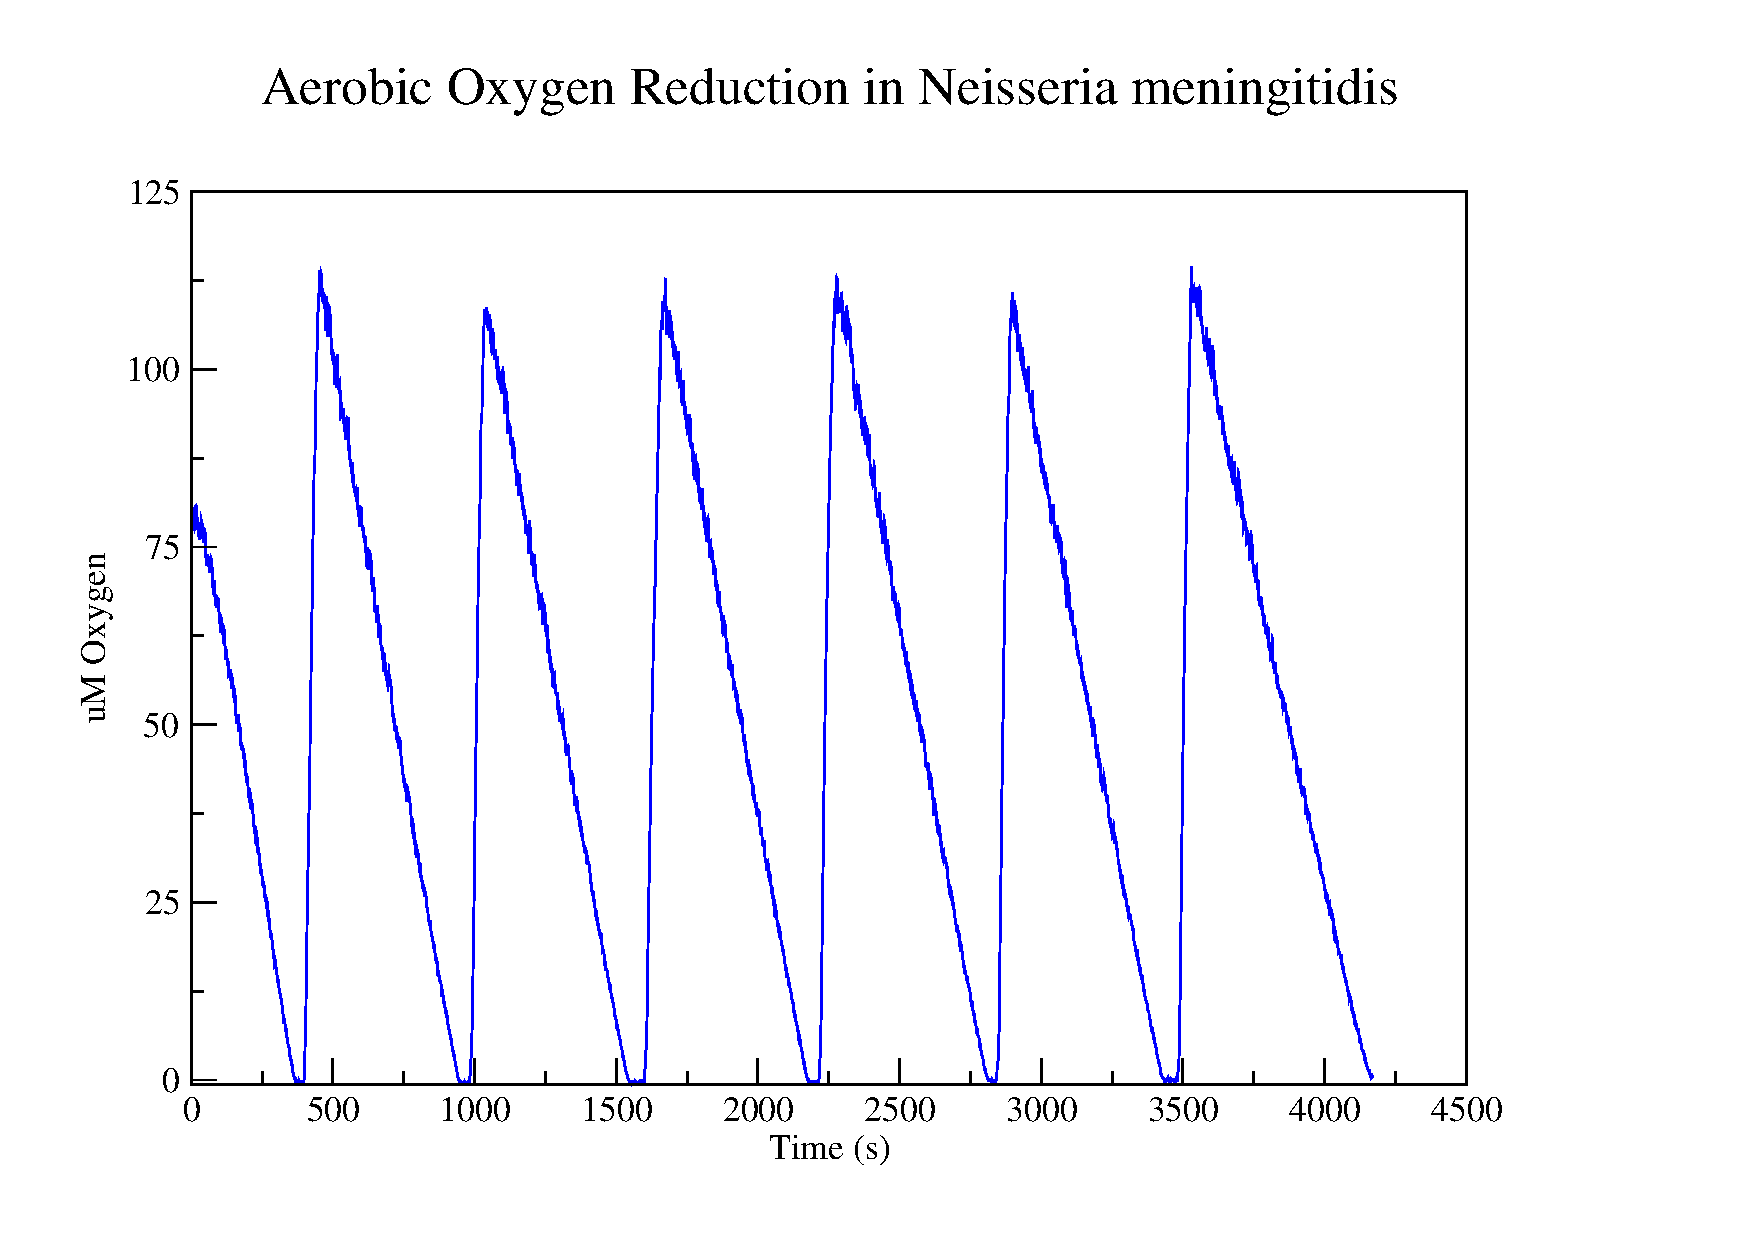
\includegraphics[width=14cm, trim=75px 50px 125px 25px]{./05-oxygenreduction/data/repeatable_o2.pdf}
 % mc58-chl-o2-util.pdf: 842x595 pixel, 72dpi, 29.70x20.99 cm, bb=0 0 842 595
 \caption[Highly repeatable oxygen reduction]{{\bf Highly repeatable oxygen reduction.} This shows an oxygen reducing culture being repeatedly aerated after oxygen depletion with very similar rates of subsequent oxygen reduction
 \label{fig:oxy_repeatable_chl}}
\end{figure}
\afterpage{\clearpage}

\begin{figure}[p]
 \centering
 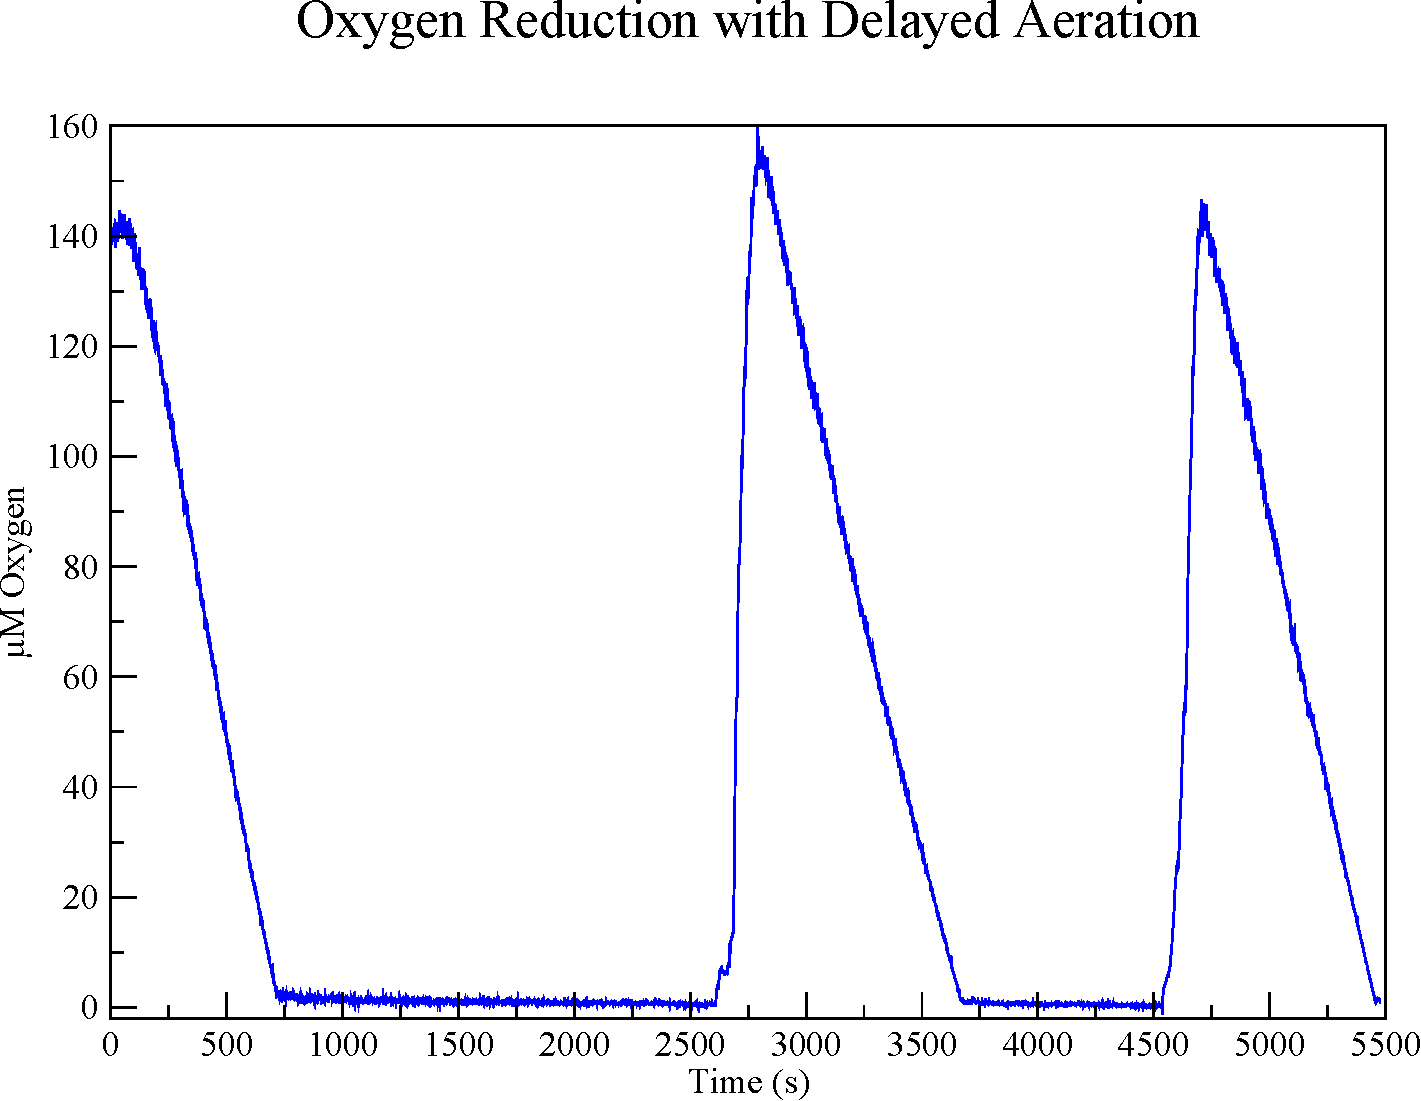
\includegraphics[width=14cm, trim=75px 50px 125px 25px]{./05-oxygenreduction/data/o2_delay.pdf}
 % repeatable-oxygen-utilisation-in-mc58.png: 640x480 pixel, 72dpi, 22.58x16.93 cm, bb=0 0 640 480
 \caption[Aerating oxygen reducing cultures with significant delay]{{\bf Aerating oxygen reducing cultures with significant delay.} The oxygen reducing ability of \Nm{} can be robust as evidenced by the 1000s delays between aeration with no change in subsequent respiration rate. Also of note is that nitric oxide concentration is not changing, suggesting that reduction of nitrite is not occurring either.
 \label{fig:repeat_oxy_with_delay}}
\end{figure}
\afterpage{\clearpage}

\subsubsection{Generation of Prior Probability Distributions}
In accordance with the integrative scheme that was introduced in Chapter \ref{chap:paramest}, An attempt was made to estimate the distributions of the parameters involved in modelling these data. In order to do this probability distributions were needed to act as priors to feed into the estimation system as this is required for a Bayesian approach. These probability distributions were generated from data obtained in the published literature, which is described in Chapter \ref{chap:model}, and preliminary experimental data. It was assumed that all the prior probabilities would be log-normally distributed, therefore the distributions  used were created under the following scheme:
\begin{itemize}
\item Where the literature value had bounds associated with it (i.e. published with $\pm{}$ values), the bounds were assumed to cover $3 \sigma$ of the normal distribution. Thus the variance used for the lognormal distribution is $\left(\frac{bounds}{3}\right)^2$ with narrow upper and lower limits.
\item Where the literature value has no bounds associated with it (i.e. published as a single figure), the bounds were assumed to be $\pm 10\%$ of the literature value, and this was used as $\sigma$. Wider upper and lower limits were used in these cases.
\item Where there are no literature values available, the value was estimated based on preliminary experimental data and bounds of $\pm 10\%$ were used again. In this case upper and lower limits for the distribution were made very wide to try and accommodate for incorrect assumed prior values.
\end{itemize}

\noindent With reference to the above, the values required to create prior probability distributions from Table \ref{tab:ps} in Chapter \ref{chap:model} are shown in Table \ref{tab:oxyProbstat}.

\begin{table}[h]%needs to be 'here' as section is short
\renewcommand{\arraystretch}{1.5}
\begin{center}
\begin{tabular}{cccc|cccc}
\toprule
\textbf{Parameter} && ${\bar{x}}$ & $\sigma^2$ & \textbf{Parameter} && ${\bar{x}}$ & $\sigma^2$\\
\midrule
$k_1$ && 415 & 191.36 & X && 3.97 & 0.018\\
$k_3$ && 3 & 0.01 & C && 0.03 & $1\times 10^{-6}$\\
$\beta$ && 0.00014 & $2.18\times 10^{-11}$ & $Q_a$ && 0.24 & $6.4\times 10^{-5}$ \\
g && 0.847 & 0.0008 & $X_a$ && 3.176 & 0.011 \\
f && 8.749 & 0.085 & $C_a$ && 0.024 & $6.4\times 10^{-7}$ \\
Q && 0.3 & 0.0001\\
\bottomrule
\end{tabular}
\end{center}
\caption[First Prior Probability Table]{{\bf Prior Probability Table} This table shows the prior means and variances used to create lognormal distributions to be used as the prior probability distributions.
\label{tab:oxyProbstat}}
\end{table}

\noindent A graphical representation of the data in Table \ref{tab:oxyProbstat}, the initial probability distributions used to start the Monte-Carlo run are shown in Figure \ref{fig:oxypriors}.% As can be seen, very little information is readily available in the literature to populate the model.

%lbrt
\begin{figure}[p]
 \centering
 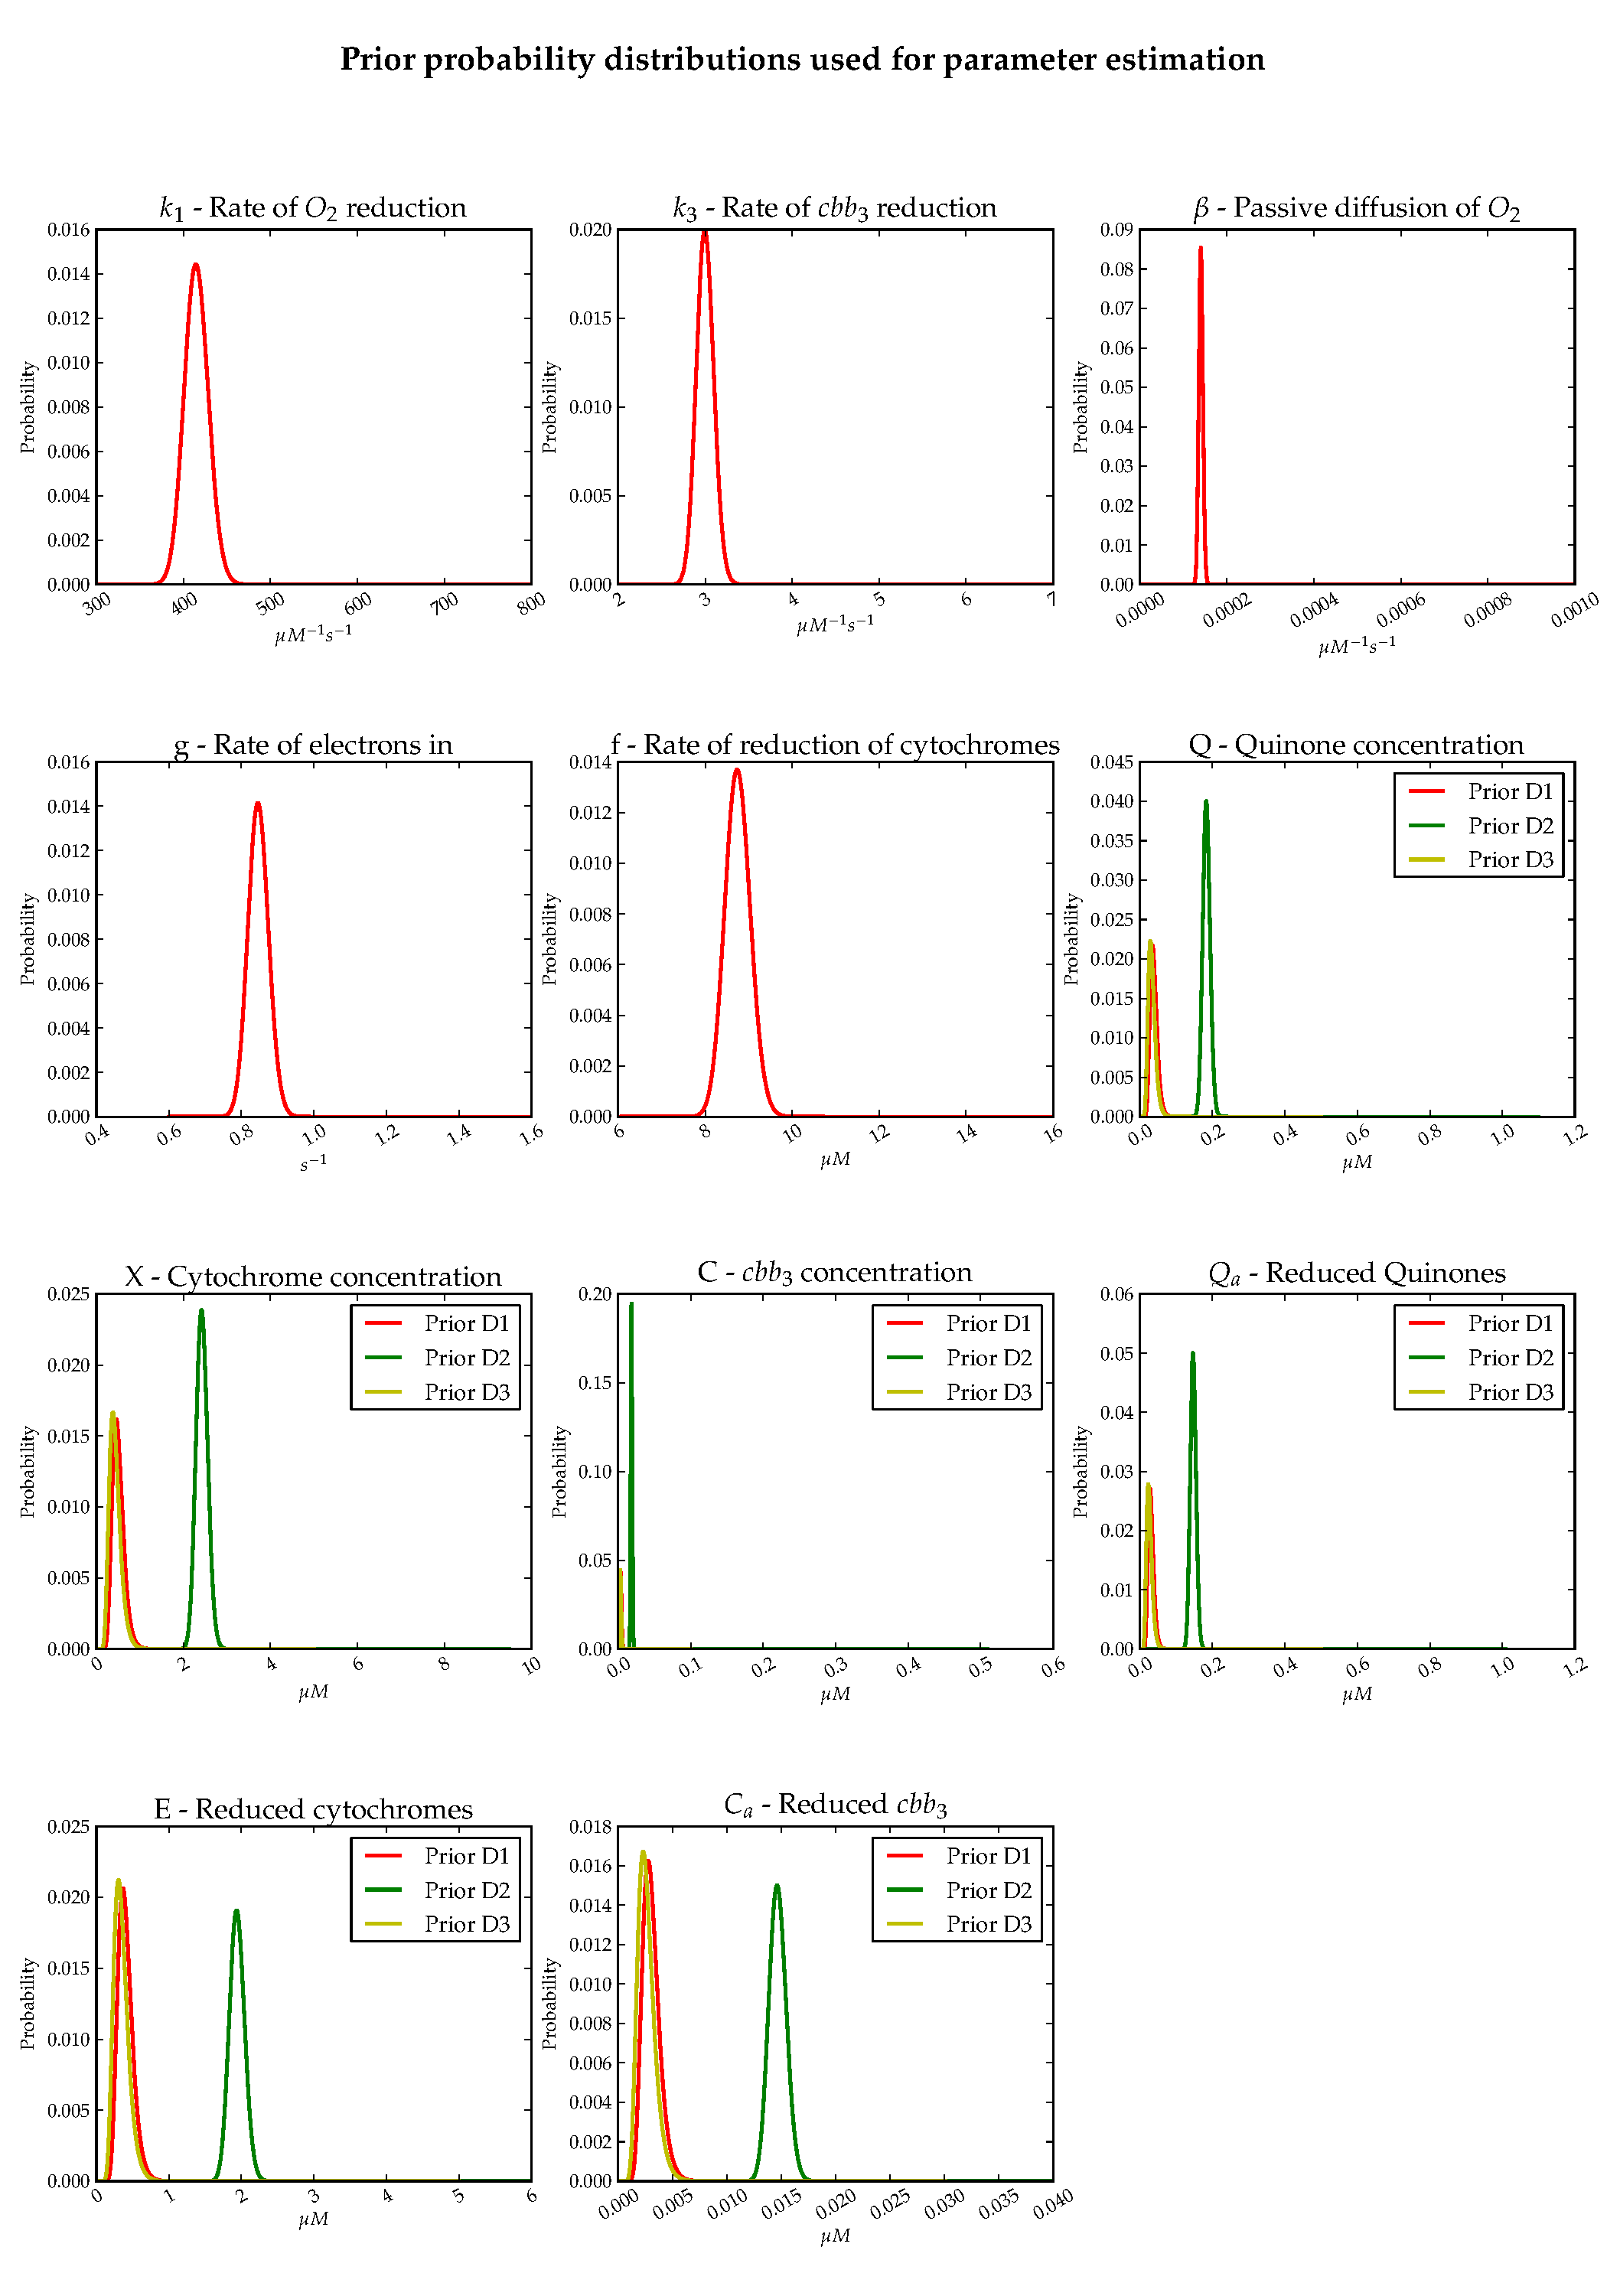
\includegraphics[width=15cm, trim=0cm 0cm 0cm 0cm]{./05-oxygenreduction/data/priors1.pdf}
 % priors.pdf: 1008x1008 pixel, 72dpi, 35.56x35.56 cm, bb=0 0 1008 1008
 \caption[Prior probability distributions for oxygen reduction]{{\bf Prior probability distributions for oxygen reduction}. These are the probability distributions used as priors by the parameter estimation algorithm.
 \label{fig:oxypriors}}
\end{figure}
\afterpage{\clearpage}

\subsubsection{Initial Parameter Estimation Results}
The parameter estimation process produces a large amount of output data which can be processed. Included in these data are the best simulation results from each run. Best is defined here as the simulation with the highest likelihood, i.e. the one with the closest match to the experimental data. For the oxygen reduction training datasets, of which there are 3, each was run 20 times for 20,000 iterations. This lower iteration count was chosen as a compromise between execution time and statistical accuracy. In fact given that the burn-in time for these runs was relatively short, 20,000 iterations still provides plenty of data. A representative example of the simulated data is shown in Figure \ref{fig:o2sim}. This figure was generated from the set of parameters that produced the most fit output compared to the input dataset.

%lbrt
\begin{figure}[p]
 \centering
 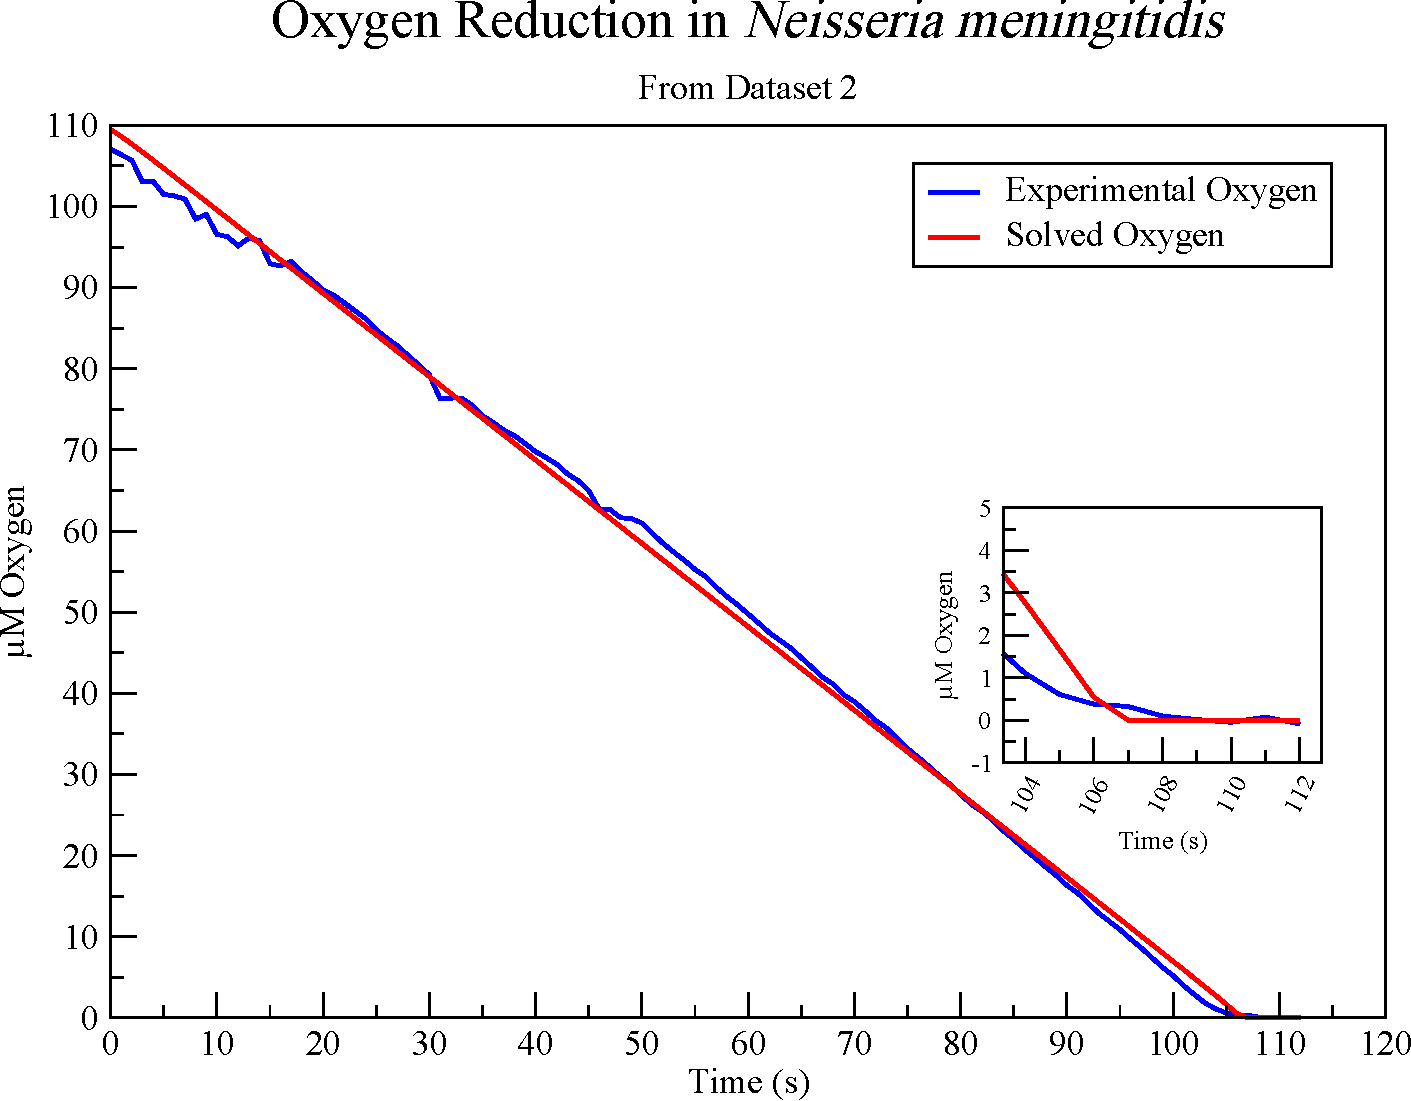
\includegraphics[width=14cm, trim=2cm 1cm 4cm 1cm]{./05-oxygenreduction/data/o2sim.pdf}
 % o2sim.eps: 0x0 pixel, 300dpi, 0.00x0.00 cm, bb=0 0 794 595
 \caption[{Oxygen Reduction in \textit{Neisseria meningitidis}.}]{{\bf Oxygen Reduction in \textit{Neisseria meningitidis}.} This dataset shows the simple linear reduction of Oxygen in aerobic conditions. The high affinity of $\mathrm{cbb}_3$ for oxygen is evidenced by very little non-linearity at low oxygen concentrations. The solved output is a representative result of the parameter estimation system.
 \label{fig:o2sim}}
\end{figure}
\afterpage{\clearpage}
%\begin{figure}[tbp]
 %\centering
 %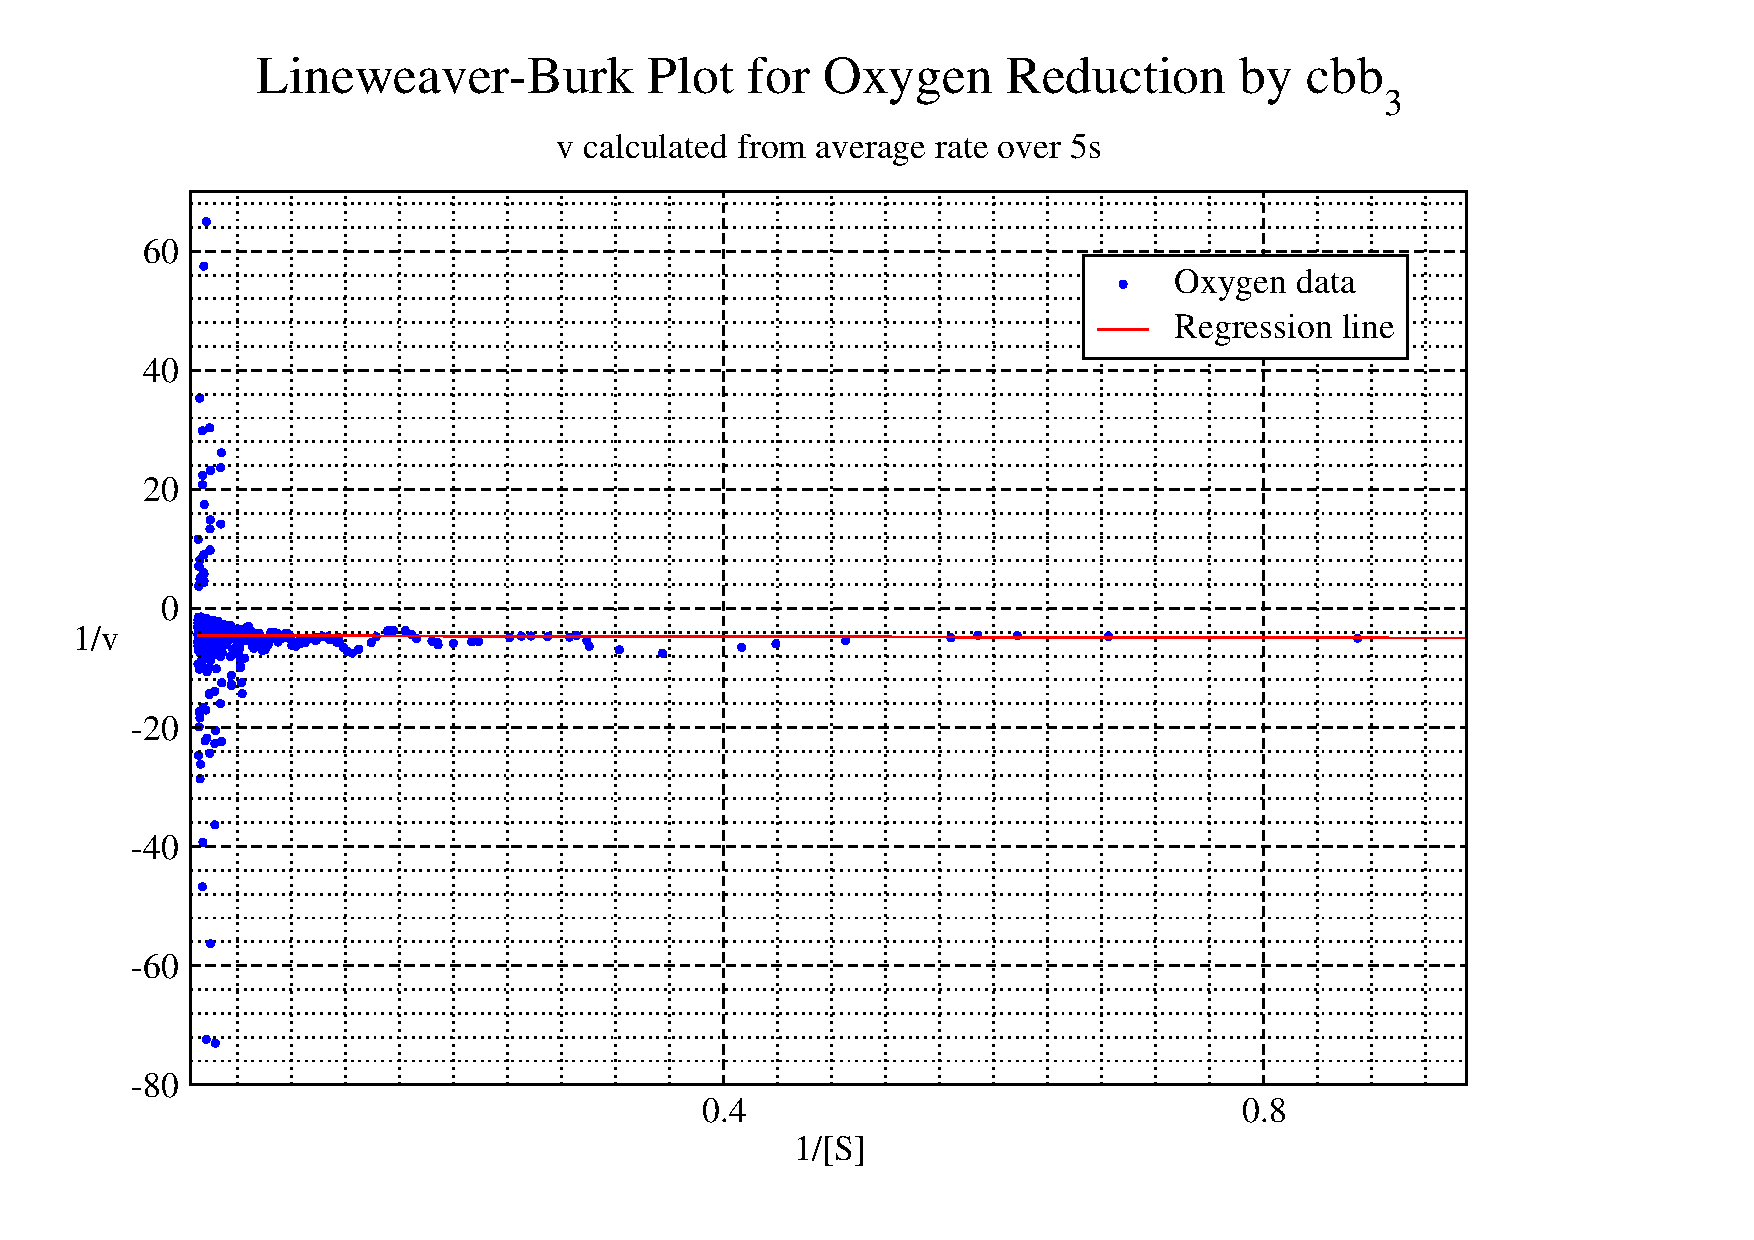
\includegraphics[height=10cm, trim=2cm 1cm 4cm 1cm]{./05-oxygenreduction/data/lbplot.pdf}
 % lbplot.pdf: 842x595 pixel, 72dpi, 29.70x20.99 cm, bb=0 0 842 595
%\end{figure}


Initially the simulation results are not particularly good fits compared to the experimental data and as such have low likelihoods (the internal representation is actually the inverse of the likelihood, so this value is high). As the parameter estimation progresses the likelihood reduces as the simulated result gets closer and closer to the experimental data. Quite often this does not take many iterations and a representative plot showing how the simulation's likelihood increases (internal representation decreases) is shown in Figure \ref{fig:oxy_fitness}. The initial period where the likelihood is low (internal representation high) up until the point it settles at a higher value (internal representation low) is classed as ``burn-in'' and is discarded when generating posterior distributions.

\begin{figure}[p]
 \centering
 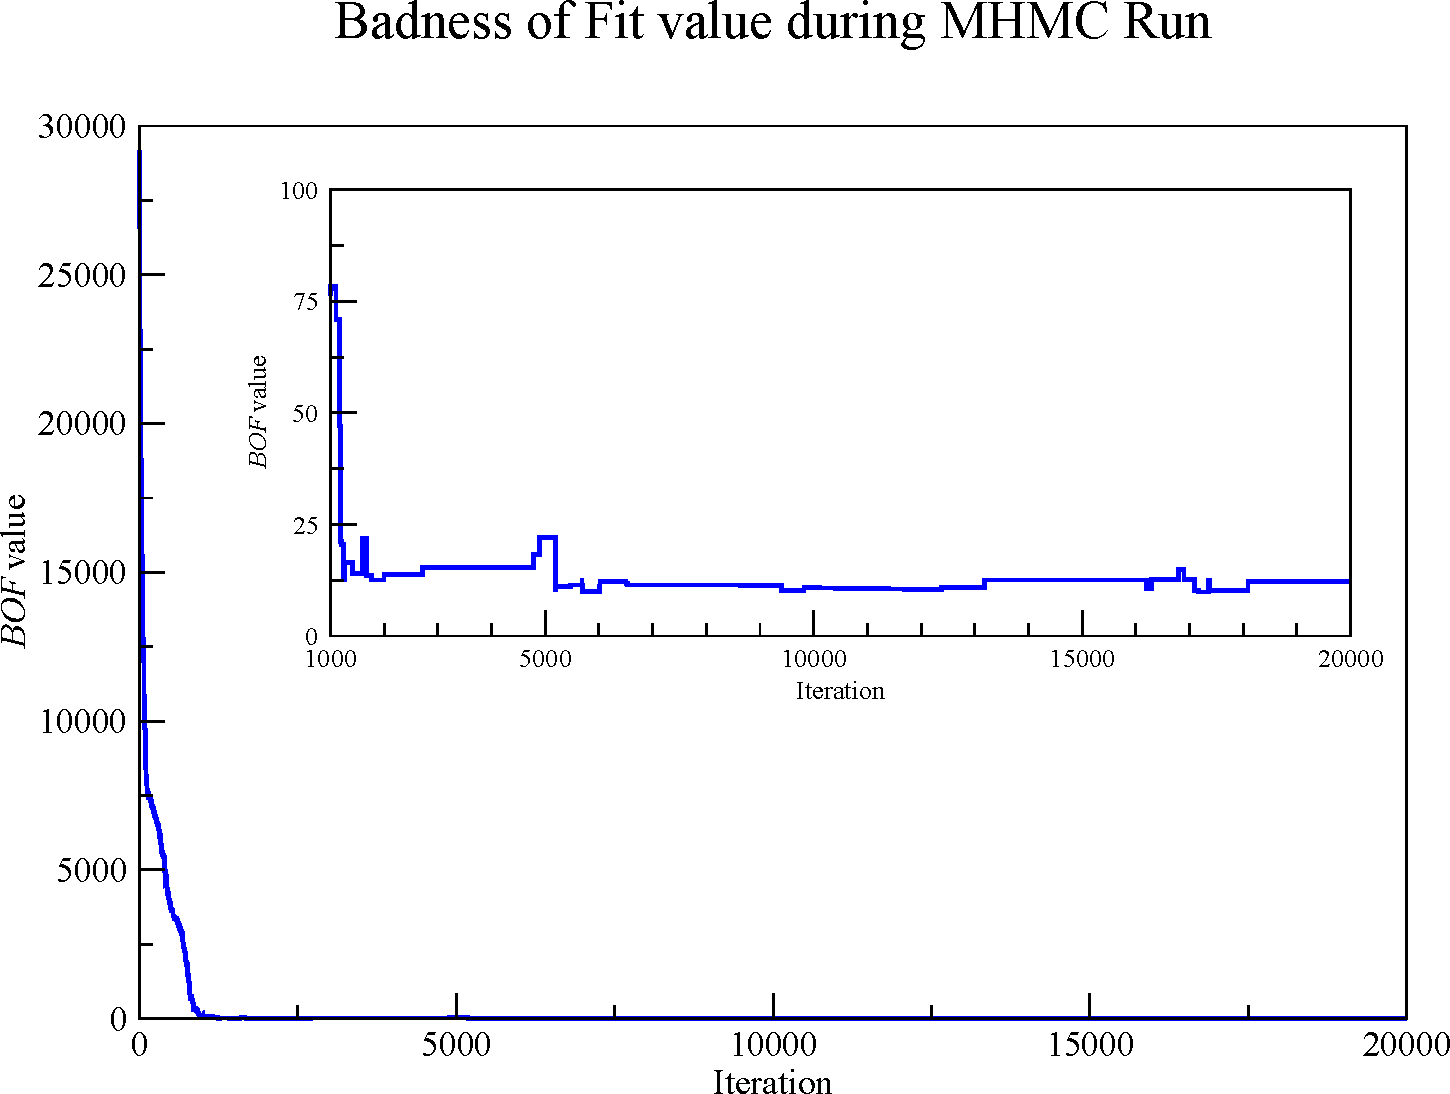
\includegraphics[width=14cm, trim=75px 50px 125px 25px]{./05-oxygenreduction/data/o2_fitness.pdf}
 % repeatable-oxygen-utilisation-in-mc58.png: 640x480 pixel, 72dpi, 22.58x16.93 cm, bb=0 0 640 480
 \caption[Simulation likelihood improves as parameter estimation progresses]{{\bf Simulation likelihood improves as parameter estimation progresses.} This is a representative figure constructed from a single run on one dataset. Initially the internal representation of likelihood is high showing that the simulated result does not match the experimental dataset. As the parameter estimation algorithm progresses, the internal representation decreases as the simulated result approaches the experimental dataset. The inset shows a zoomed in view of the likelihood after the ``burn-in'' process has finished.
 \label{fig:oxy_fitness}}
\end{figure}
\afterpage{\clearpage}

Each of the parameters that are to be estimated produces a trajectory of values for each run of the estimation algorithm. These trajectories are used to generate the posterior probability distributions required for Bayesian inference in subsequent steps. During the ``burn in'' period the parameter values can be observed to change rapidly from one iteration to the next as they approach their optimum values. Once the ``burn in'' has completed the values settle and produce largely flat trajectories with minor deviations around the optimum value. This settled region is used as the source for generating the posterior probability distributions. Figure \ref{fig:k3s} shows the the trajectories from each simulation run on a single dataset for the $k_3$ parameter.

\begin{figure}[p]
 \centering
 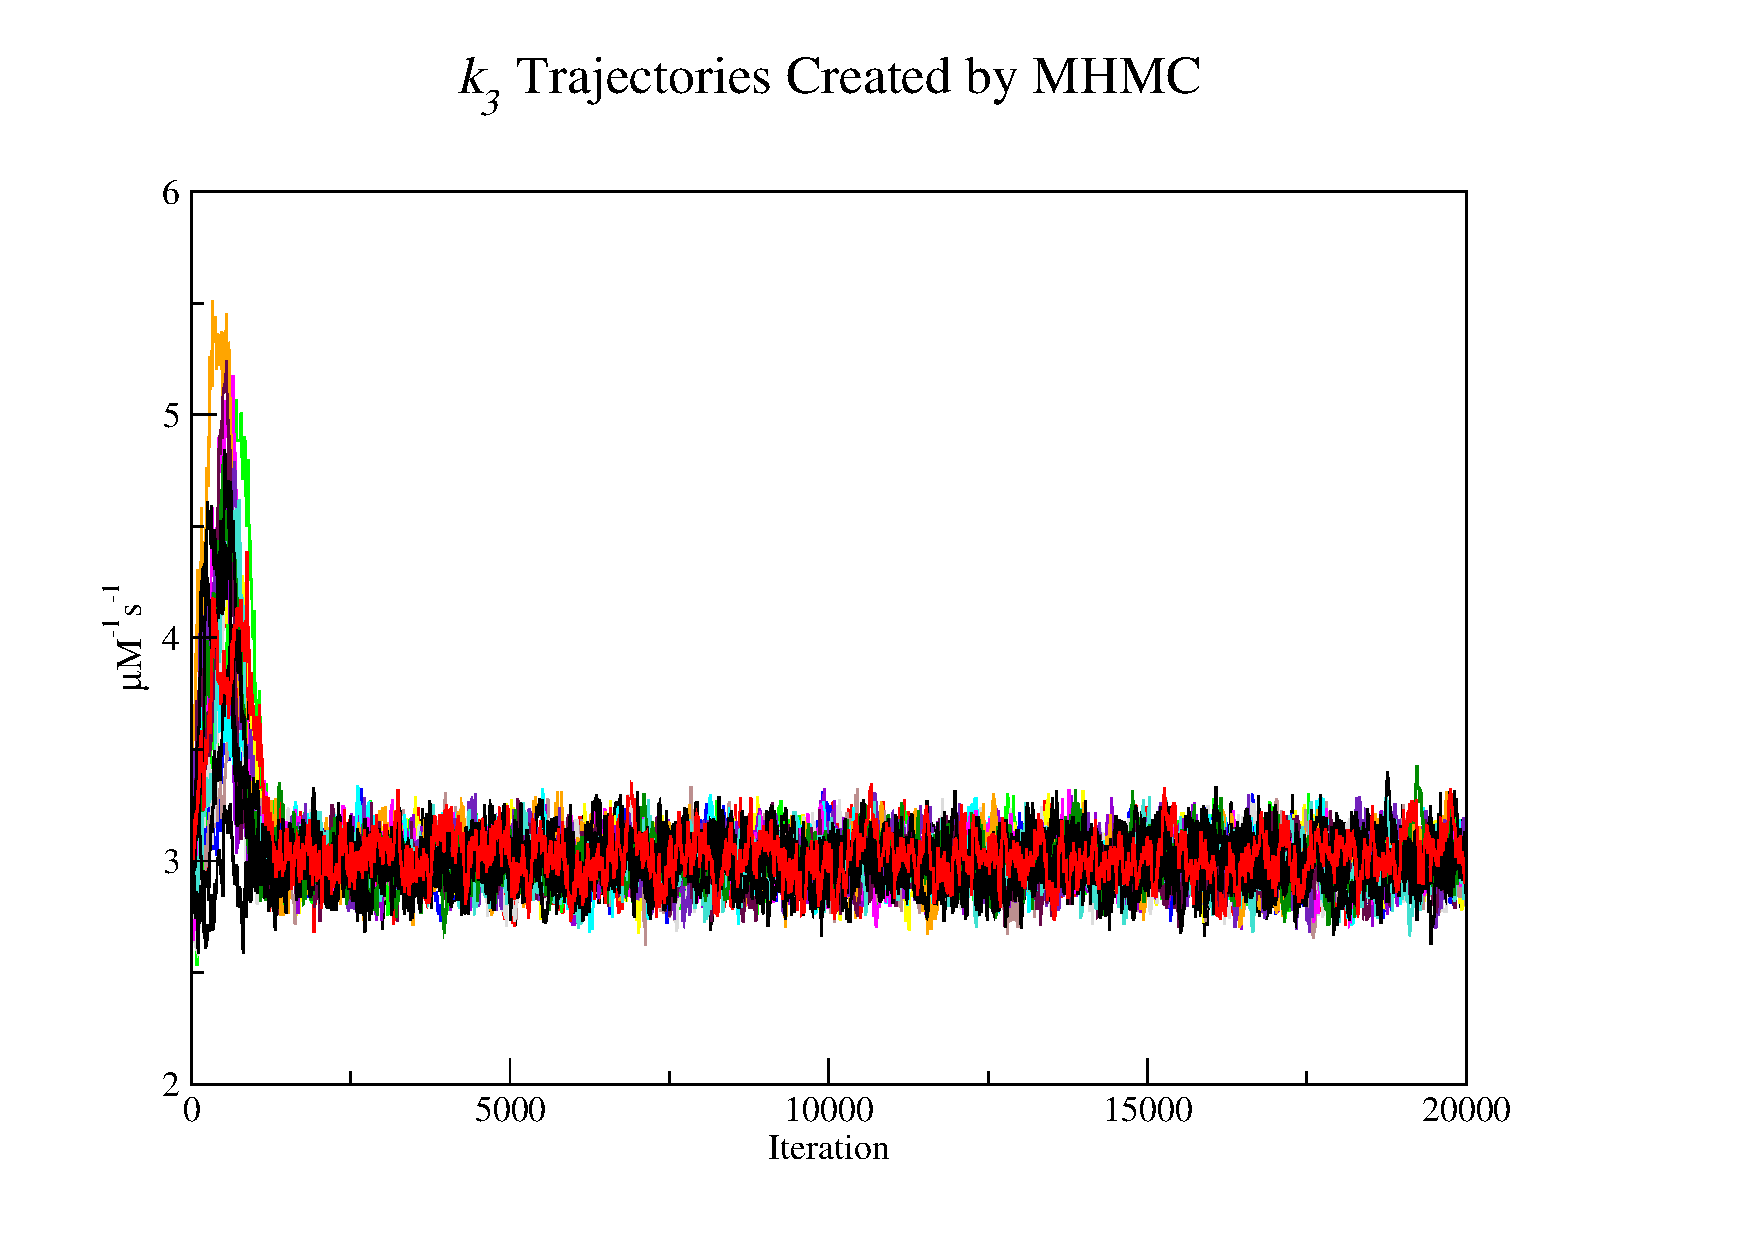
\includegraphics[width=14cm, trim=75px 50px 125px 25px]{./05-oxygenreduction/data/k3s1.pdf}
 % repeatable-oxygen-utilisation-in-mc58.png: 640x480 pixel, 72dpi, 22.58x16.93 cm, bb=0 0 640 480
 \caption[Individual parameter trajectories for multiple runs on the same experimental dataset]{{\bf Individual parameter trajectories for multiple runs on the same experimental dataset.} This figure shows the trajectories for the same parameter, in this case $k_3$ - the rate constant for \cbbthree{} reduction, from 20 individual runs of parameter estimation upon the same input data. The trajectories show clear convergence after the ``burn-in'' period.
 \label{fig:k3s}}
\end{figure}
\afterpage{\clearpage}

Not all parameters in this stage of the model will produce trajectories like the one shown, as if there is a great deal of freedom as to what value a particular parameter can take without drastically decreasing the likelihood it will be accepted by the parameter estimation algorithm. In this case the trajectories will not converge, and will ultimately produce a wide probability distribution. This is not necessarily indicative of a problem however, as this output still contains information that can be used in the next stage of parameter estimation with new datasets.

The trajectories above are processed to produce probability distributions given as histograms. The ``burn in'' is discarded and the settled data is then binned and counted. For the datasets used, the burn-in period was 1500 iterations. These histogram probabilities are then assigned as the posterior distributions and in turn are used directly as prior probability distributions for new datasets. For simplicities sake when referring to the distribution of individual parameters for purposes of comparison, these histograms are transformed into log-normal distribution such that they can be represented by two numbers, $\bar{x}$ - the mean, and $\sigma^2$ - the variance.

The posterior probability distributions generated from the three experimental datasets, each started with 20 runs are shown in Figure \ref{fig:oxyposteriors}. In the case of parameters which represent concentrations, such as $X$ and $C$, the concentrations of cytochromes and \cbbthree{} respectively, the individual dataset probability distributions are shown, as they cannot be sensibly combined, and it emphasises the fact that the datasets were different.

\begin{figure}[p]
 \centering
 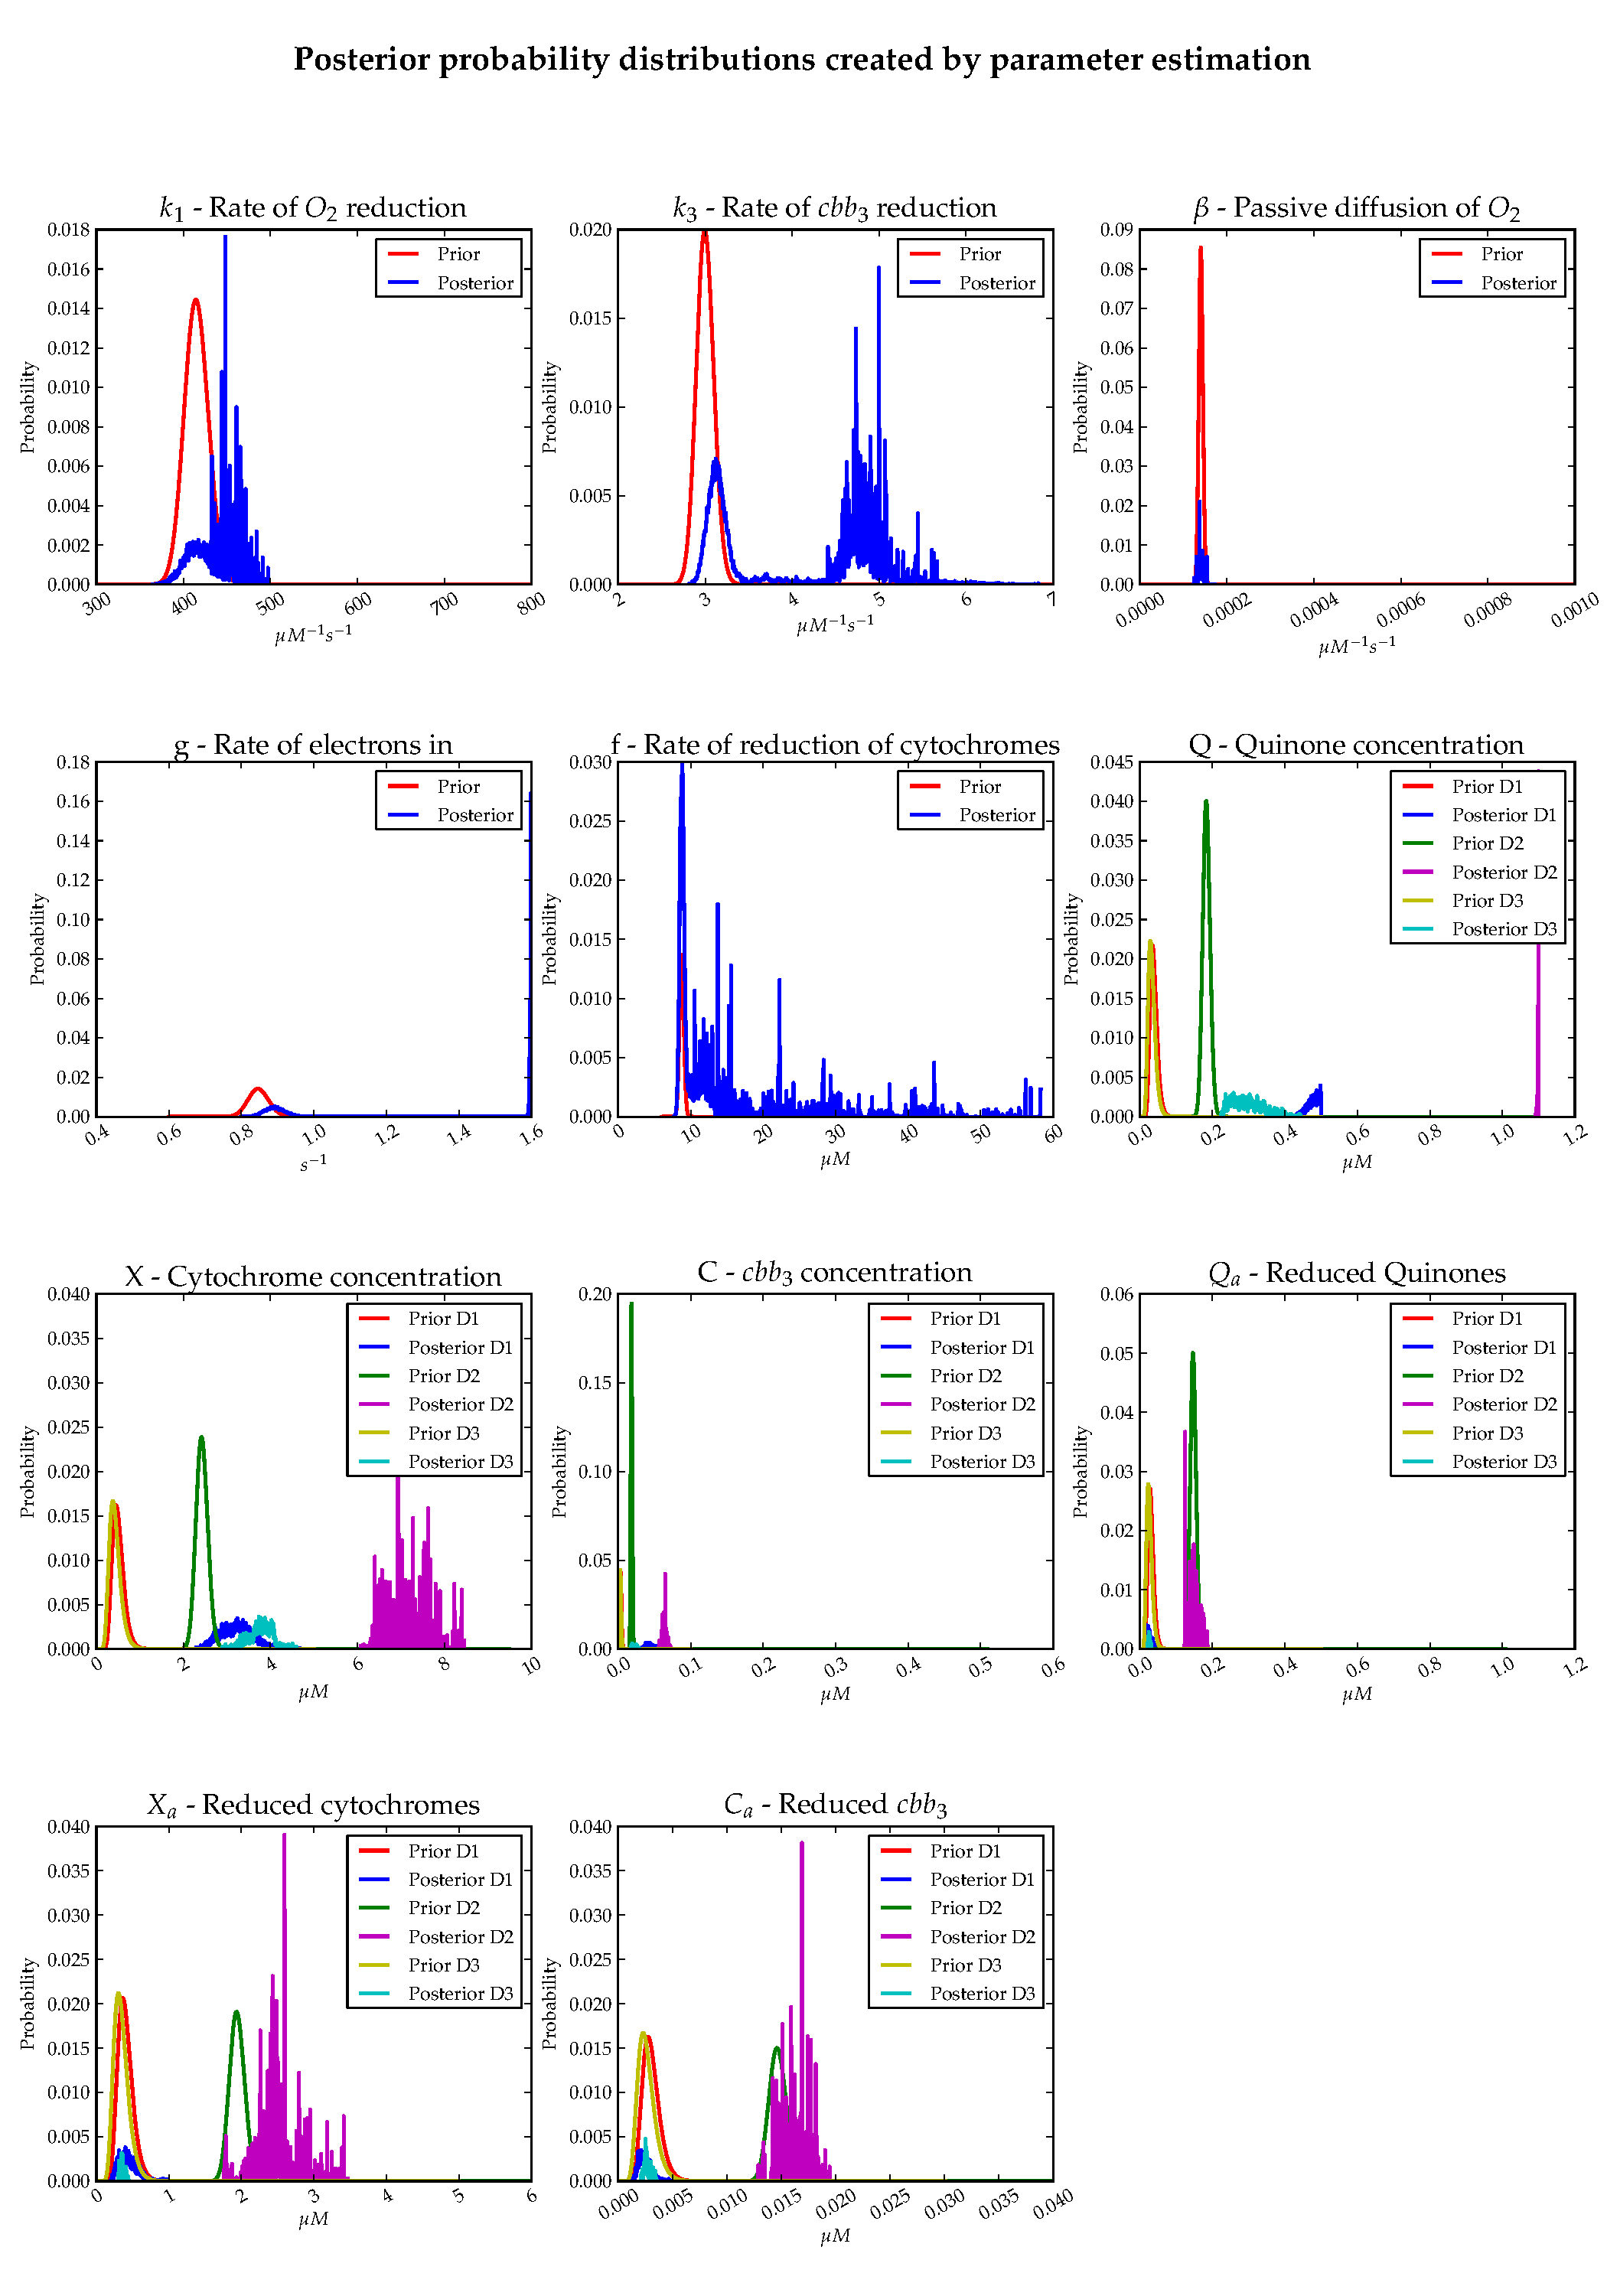
\includegraphics[width=15cm, trim=0cm 0cm 0cm 0cm]{./05-oxygenreduction/data/posteriors1.pdf}
 % posteriors.pdf: 1008x1008 pixel, 72dpi, 35.56x35.56 cm, bb=0 0 1008 1008
 \caption[Posterior probability distributions for oxygen reduction]{{\bf Posterior probability distributions for oxygen reduction}. These are the probability distributions generated by parameter estimation on 3 oxygen reduction datasets. These have been overlaid onto the prior probability distributions used by the parameter estimation algorithm, also shown in Figure \ref{fig:oxypriors}.
 \label{fig:oxyposteriors}}
\end{figure}
\afterpage{\clearpage}

As can be seen from the posterior distributions, the parameter estimation algorithm has not satisfactorily produced posterior distributions that are contained within the bounds of the prior distributions whilst also still managing to fit to the experimental data. This is especially true of the concentration of $Q$, where the Markov-chain has tended towards the upper limit of the input prior distribution. This suggests that the prior distribution for $Q$ is incorrect, with a mean that is possibly as much as $10\times$ too low, and with a variance that is too small, as the parameter estimation algorithm has attempted to increase the value of $Q$ right up to the upper limit of the input distribution. This incorrect value for $Q$ is probably the cause of several of the other distributions being flatter and outside of the main body of their prior distributions. Another interesting observation is that the distribution for $k_3$ shows a distinct bi-modality, however this is quite likely to be an artefact of the parameter estimation algorithm. The left-most region of the bimodal distribution could be caused by the natural bias of the algorithm for values within more likely regions of the prior probability distribution. If this is the case, the right-most region is the ``true'' probability distribution where the increase in likelihood of fitting outweighs the fact that the values selected have a low probability of being selected from the prior distribution. Assuming this is the case, the prior distribution may also be incorrect for $k_3$, but the shape of the posterior distribution may also be directly caused by the more obviously incorrect prior distribution of $Q$.

Since the posterior probability distributions generated at this stage cannot be used as priors for the reasons described above, the prior distributions were altered to try and correct them. These alterations are described in the next section.

%FIXME -> bimodal probability distribution not shown
%Additionally $k_1$, the rate constant for reduction of Oxygen by \cbbthree{} showed bimodality (not shown currently) \textit{and} a very broad range. The bimodal nature of this distribution was not matched in any of the other parameters. This parameter is the last rate constant in the ETC of oxygen reduction, so it is quite possible that the rate limiting steps are in the previous stages of the ETC and thus in the parameter estimation system $k_1$ essentially becomes ``free'', and could be the reason for poor fitting at lower oxygen concentrations.

%Some of the posterior probability distributions appear to have expanded outside their prior bounds. I am fairly certain that this is not an error and that samples \textit{are} being taken from the prior distributions, but rather that the prior distributions were sufficiently incorrect that the penalty for selecting a parameter value from the prior distribution which is very unlikely is outweighed by the large increase in likelihood that this affords.

\subsubsection{Secondary Prior Probability Distributions}
\begin{table}[h]%needs to be 'here' as section is short
\renewcommand{\arraystretch}{1.5}
\begin{center}
\begin{tabular}{cccc|cccc}
\toprule
\textbf{Parameter} && ${\bar{x}}$ & $\sigma^2$ & \textbf{Parameter} && ${\bar{x}}$ & $\sigma^2$\\
\midrule
$k_1$ && 415 & 956.8 & X && 3.97 & 0.18\\
$k_3$ && 3 & 0.1 & C && 0.03 & $1\times 10^{-5}$\\
$\beta$ && 0.00014 & $2.18\times 10^{-11}$ & $Q_a$ && 0.24 & $6.4\times 10^{-5}$\\
g && 0.847 & 0.008 & $X_a$ && 3.176 & 0.011\\
f && 8.749 & 3.0 & $C_a$ && 0.024 & $6.4\times 10^{-7}$\\
Q && 3 & 0.01\\
\bottomrule
\end{tabular}
\end{center}
\caption[Second Prior Probability Table]{{\bf Prior Probability Table} This table shows the prior means and variances used to create lognormal distributions to be used as the prior probability distributions.
\label{tab:oxyProbstat1}}
\end{table}
\noindent A graphical representation of the data in Table \ref{tab:oxyProbstat1}, the initial probability distributions used to start the Monte-Carlo run are shown in Figure \ref{fig:oxypriors1}.
%lbrt
\begin{figure}[p]
 \centering
 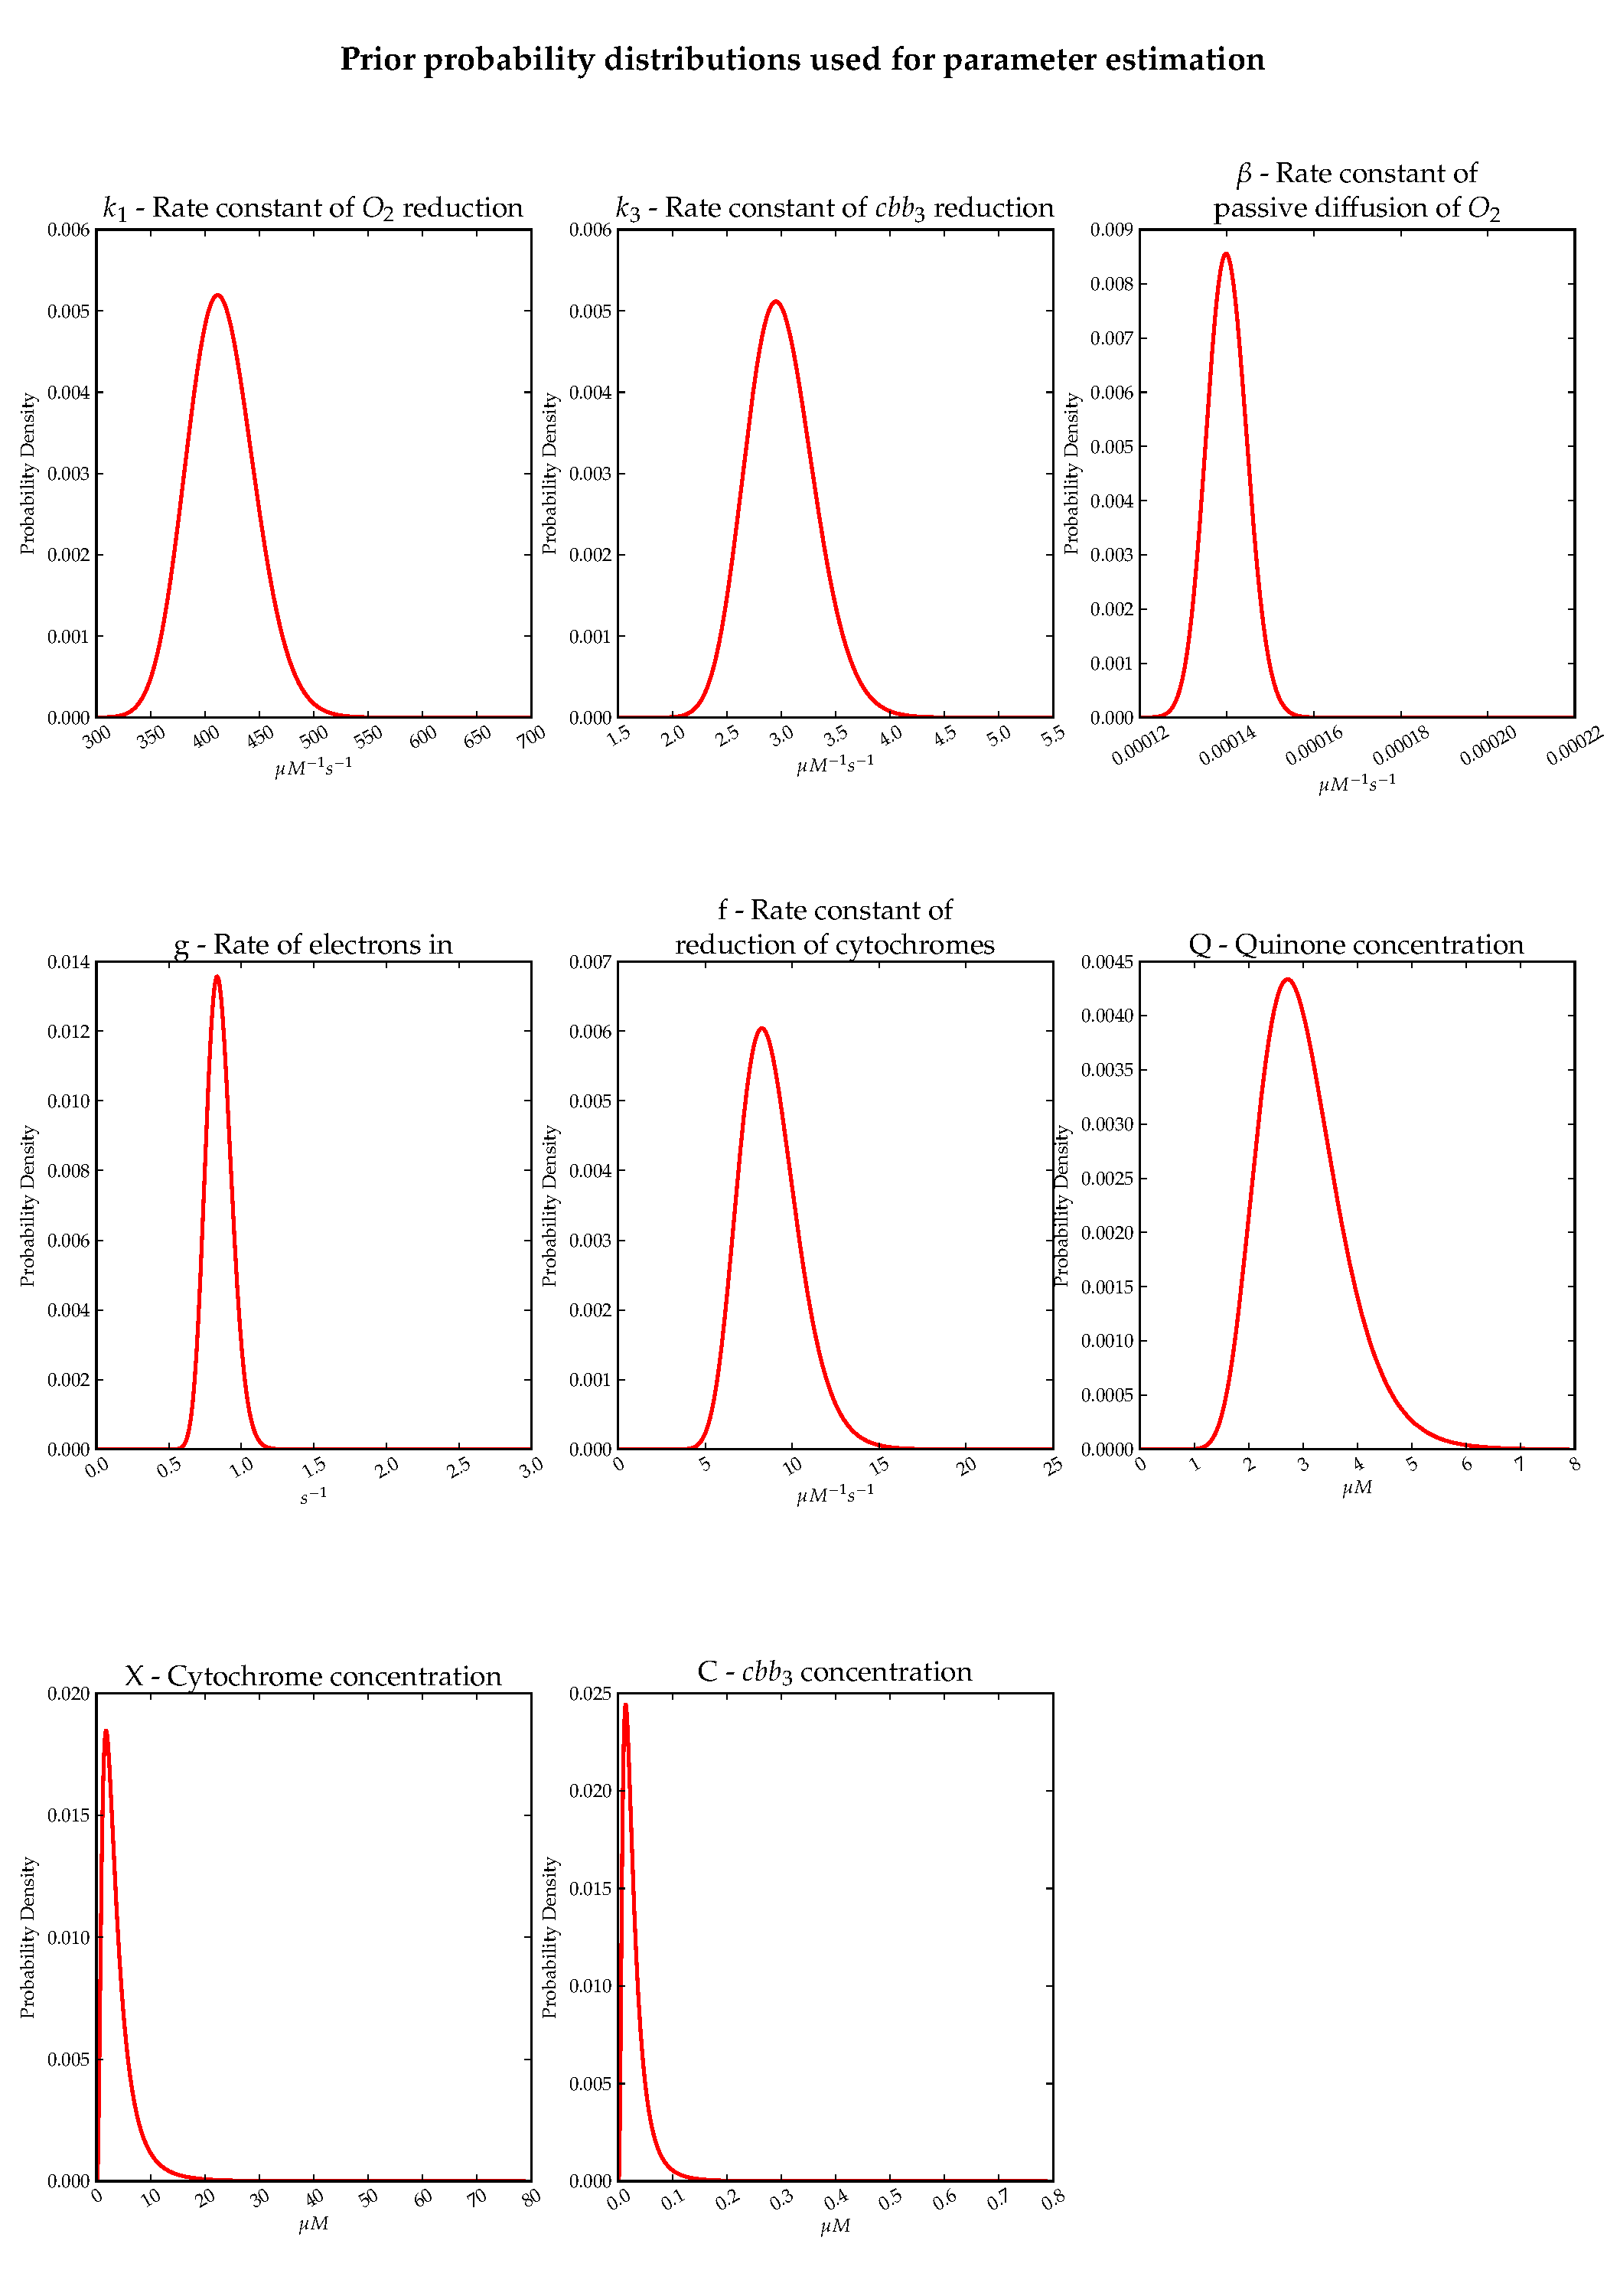
\includegraphics[width=15cm, trim=0cm 0cm 0cm 0cm]{./05-oxygenreduction/data/priors2.pdf}
 % priors.pdf: 1008x1008 pixel, 72dpi, 35.56x35.56 cm, bb=0 0 1008 1008
 \caption[Prior probability distributions for oxygen reduction]{{\bf Prior probability distributions for oxygen reduction}. These are the probability distributions used as priors by the parameter estimation algorithm.
 \label{fig:oxypriors1}}
\end{figure}
\afterpage{\clearpage}
\subsubsection{Analysis of Convergence}
It is possible to calculate the degree of convergence of the parameters from the Monte Carlo trajectories using the R statistic introduced by \citet{Gelman1992} and \citet{Brooks1998}. This statistic produces in a single figure what could interpreted from the posterior probability distributions as it is essentially a measure of how close the trajectories have become towards the end of said trajectory. This statistic is calculated on the trajectories from multiple runs \textit{for each parameter individually}. The R statistic was calculated using the \textit{Bolstad2}\cite{Curran2011} library for R\cite{RDevelopmentCoreTeam2010}.
\begin{table}[h]%needs to be 'here' as section is short
\renewcommand{\arraystretch}{1.5}
\begin{center}
\begin{tabular}{ccccccc}
\toprule
& & \multicolumn{2}{c}{\textbf{Priors}} & \multicolumn{2}{c}{\textbf{Posteriors}} & \\
\textbf{Parameter} && ${\bar{x}}$ & $\sigma^2$ & ${\bar{x}}$ & $\sigma^2$ & $\mathbf{R_{All}}$\\
\midrule
$k_1$ && 415 & 956.8 & N/A & N/A & N/A\\
$k_3$ && 3 & 0.1 & N/A & N/A & N/A\\
$\beta$ && 0.00014 & $2.18\times 10^{-11}$ & N/A & N/A & N/A\\
g && 0.847 & 0.008 & N/A & N/A & N/A\\
f && 8.749 & 3.0 & N/A & N/A & N/A\\
Q && 3 & 0.01 & N/A & N/A & N/A\\
X && 3.97 & 0.18 & N/A & N/A & N/A\\
C && 0.03 & $1\times 10^{-5}$ & N/A & N/A & N/A\\
$Q_a$ && 0.24 & $6.4\times 10^{-5}$ & N/A & N/A & N/A\\
$X_a$ && 3.176 & 0.011 & N/A & N/A & N/A\\
$C_a$ && 0.024 & $6.4\times 10^{-7}$ & N/A & N/A & N/A\\
\bottomrule
\end{tabular}
\end{center}
\caption[Gelman-Rubin Convergence Statistic]{{\bf Gelman-Rubin Convergence Statistic} This table shows the prior and posterior means and standard deviations in addition to the Gelman-Rubin Convergence statistic for all chains.
\label{tab:oxyRstat}}
\end{table}
Table \ref{tab:oxyRstat} shows the R statistics obtained from the trajectories run for oxygen reduction parameter estimation. The R statistic is a measure of scale-reduction, and fully converged trajectories will have a value of $1.0$ whereas trajectories which have not converged will have values greater than 1 with the magnitude depending on how far away from converging they are. As can be seen in the table it appears that the majority of the trajectories have not converged with the exception of Q, the quinone concentration. This is not completely unexpected, as there are a larger number of parameters in the model than are required to fit the experimental data and thus the potential range of parameter values is broad at this stage. I was therefore not worried about the lack of convergence at this point as with subsequent, more complex datasets the range of potential parameter values will decrease, allowing the trajectories to converge more easily.

\subsubsection{Analysis of Correlation}
Given the large number of parameters, and the simple form of the experimental data it is quite likely that a number of the parameters will be correlated with one another. This effect should also be exacerbated at this stage due to the limited constraints (by virtue of wide prior probabilities) on the ranges of values that parameters can take. In order to investigate this I constructed a correlation matrix by calculating the Pearson's Product-Moment Correlation Coefficient for each of the parameters. This value provides the direction of correlation as indicated by the sign, and the degree of linearity as indicated by the magnitude. A positive correlation indicates that as the value of one parameter increases, the other increases also. A negative correlation indicates that as the value of one parameter increases, the other decreases.

The upper-triangle correlation matrix is shown in Figure \ref{tab:oxyregress} and was constructed by concatenating all the trajectories created by the parameter estimation system (discarding the burn-in) together and the Pearson's Product-Moment Correlation Coefficient calculated for each combination. The matrix is upper-triangle only as the lower triangle is a duplicate of the same data. The diagonal is shown in grey as it is not useful data since the correlation of X against X is always 1.
%\begin{landscape}
\begin{table}[p]
\setlength{\tabcolsep}{5pt}
\renewcommand{\arraystretch}{1.5}
  \centering
  \rotatebox{90}{
  \begin{minipage}{24.4cm}
  \centering
  \begin{tabular}{|c|c|c|c|c|c|c|c|c|c|c|c|c|}
    \hline
    \cellcolor{dark-gray} & \cellcolor{dark-gray}$k_1$ & \cellcolor{dark-gray}$k_3$ & \cellcolor{dark-gray}$\beta$ & \cellcolor{dark-gray}g & \cellcolor{dark-gray}f & \cellcolor{dark-gray}Q & \cellcolor{dark-gray}X & \cellcolor{dark-gray}C & \cellcolor{dark-gray}$Q_a$ & \cellcolor{dark-gray}$X_a$ & \cellcolor{dark-gray}$C_a$ \\
    \hline
    \cellcolor{dark-gray}$k_1$ & \cellcolor{light-gray}$1$ & $0.28599$ & $0.013212$ & \cellcolor{orange}$0.420123$ & $0.154821$ & $0.009968$ & \cellcolor{orange}$0.369637$ & \cellcolor{orange}$0.367247$ & $0.00344$ & $0.000229$ & $0.046062$ \\
    \hline
    \cellcolor{dark-gray}$k_3$ & \cellcolor{light-gray} & \cellcolor{light-gray}$1$ & $0.008486$ & \cellcolor{orange}$0.586606$ & \cellcolor{orange}$0.351956$ & $0.002927$ & \cellcolor{orange}$0.617929$ & \cellcolor{orange}$0.681098$ & $0.000559$ & $0.001062$ & $0.012978$ \\
    \hline
    \cellcolor{dark-gray}$\beta$ & \cellcolor{light-gray} & \cellcolor{light-gray} & \cellcolor{light-gray}$1$ & $0.009472$ & $0.07071$ & $6.58\times{}10^{-5}$ & $0.001034$ & $0.019449$ & $0.006711$ & $0.055052$ & $0.002166$ \\
    \hline
    \cellcolor{dark-gray}g & \cellcolor{light-gray} & \cellcolor{light-gray} & \cellcolor{light-gray} & \cellcolor{light-gray}$1$ & \cellcolor{orange}$0.426205$ & $0.008692$ & \cellcolor{green}$0.86507$ & \cellcolor{green}$0.811637$ & $0.009455$ & $0.003244$ & $0.076195$ \\
    \hline
    \cellcolor{dark-gray}f & \cellcolor{light-gray} & \cellcolor{light-gray} & \cellcolor{light-gray} & \cellcolor{light-gray} & \cellcolor{light-gray}$1$ & $0.00461$ & \cellcolor{orange}$0.329468$ & \cellcolor{orange}$0.432466$ & $0.106478$ & $0.012951$ & $0.001404$ \\
    \hline
    \cellcolor{dark-gray}Q & \cellcolor{light-gray} & \cellcolor{light-gray} & \cellcolor{light-gray} & \cellcolor{light-gray} & \cellcolor{light-gray} & \cellcolor{light-gray}$1$ & $0.008756$ & $0.006046$ & $0.00024$ & $7.86\times{}10^{-6}$ & $0.003555$ \\
    \hline
    \cellcolor{dark-gray}X & \cellcolor{light-gray} & \cellcolor{light-gray} & \cellcolor{light-gray} & \cellcolor{light-gray} & \cellcolor{light-gray} & \cellcolor{light-gray} & \cellcolor{light-gray}$1$ & \cellcolor{green}$0.803124$ & $1.47\times{}10^{-5}$ & $3.43\times{}10^{-5}$ & $0.064213$ \\
    \hline
    \cellcolor{dark-gray}C & \cellcolor{light-gray} & \cellcolor{light-gray} & \cellcolor{light-gray} & \cellcolor{light-gray} & \cellcolor{light-gray} & \cellcolor{light-gray} & \cellcolor{light-gray} & \cellcolor{light-gray}$1$ & $0.018731$ & $7.27\times{}10^{-5}$ & $0.046421$ \\
    \hline
    \cellcolor{dark-gray}$Q_a$ & \cellcolor{light-gray} & \cellcolor{light-gray} & \cellcolor{light-gray} & \cellcolor{light-gray} & \cellcolor{light-gray} & \cellcolor{light-gray} & \cellcolor{light-gray} & \cellcolor{light-gray} & \cellcolor{light-gray}$1$ & $0.108255$ & $0.00897$ \\
    \hline
    \cellcolor{dark-gray}$X_a$ & \cellcolor{light-gray} & \cellcolor{light-gray} & \cellcolor{light-gray} & \cellcolor{light-gray} & \cellcolor{light-gray} & \cellcolor{light-gray} & \cellcolor{light-gray} & \cellcolor{light-gray} & \cellcolor{light-gray} & \cellcolor{light-gray}$1$ & $0.003167$ \\
    \hline
    \cellcolor{dark-gray}$C_a$ & \cellcolor{light-gray} & \cellcolor{light-gray} & \cellcolor{light-gray} & \cellcolor{light-gray} & \cellcolor{light-gray} & \cellcolor{light-gray} & \cellcolor{light-gray} & \cellcolor{light-gray} & \cellcolor{light-gray} & \cellcolor{light-gray} & \cellcolor{light-gray}$1$ \\
    \hline
  \end{tabular}
  \caption[Regression Analysis of Oxygen Reduction Parameters]{{\bf Regression Analysis of Oxygen Reduction Parameters.} This table shows the $R^2$ values from linear regression analysis on the combined parameter trajectories for Oxygen reduction. Parameters with high correlation have been coloured green ($R^2>0.8$) and those with moderation correlation have been coloured orange ($0.8>R^2>0.3$).
  \label{tab:oxyregress}}
  \end{minipage}
  }
\end{table}
%\end{landscape}
The correlation matrix shows that the majority of the parameters are not correlated with each other, giving very low $R^2$ values. A number of the parameters showed moderate correlation, which is to be expected. Parameters such as $k_1$ - the rate constant for reduction of oxygen - and $k_3$ - the rate constant for reduction of \cbbthree{} -  broadly speaking would increase as g - the rate of electrons in -  increased. This was expected as more electrons means higher observable rates are possible. Strong positive correlations exist between the concentrations of cytochromes (X), \cbbthree{}(C) and the rate of electrons in (g). This makes sense if higher likelihoods require an increased throughput of electrons but that cannot be achieved by increasing the size of the quinone pool. Large numbers of electrons can be reduced by the cytochromes to eventually reduce oxygen.

Interestingly there were no negative correlations observed. This is somewhat odd as it might be expected that as the reduction rates of enzymes goes down, the concentration of the enzyme increases to maintain the same overall electron throughput. It appears however that the maximum likelihood is achieved when maximising oxygen throughput.
\subsection{Discussion}
The experimental datasets showed that oxygen reduction in \Nm{} is a simple linear system with the reductase having a high affinity for oxygen demonstrated by the almost complete lack of non-linearity as oxygen concentration approaches zero. Unfortunately the degree of affinity could not be explored further as it was limited by the sampling rate of the oxygen electrode. Nonetheless this apparent simple linearity could be very easily have been modelled to a high degree of accuracy with just 2 parameters in a simple $y=-mx+c$ system. Admittedly this would not include the behaviour when the oxygen concentration reaches zero, which is that it remains so. However this essentially meant that there were a much larger number of parameters available to fit than were necessary, which lead to over-fitting of the data. The size of the parameter set meant that there were a very large set of potential combinations that would have lead to a similar result, however this was mitigated somewhat by the prior probability distributions given to the algorithm. Even so, this meant that the posterior distributions generated were very wide and therefore allowed much greater freedom for the next dataset to explore the parameter space.

With the knowledge of the underlying transport chain and the affinity of \cbbthree{} for oxygen, I expected a linear reduction of oxygen with high affinity over nearly two orders of magnitude. This was evidenced in the experimental data. It is however remarkable that this behaviour can be modelled with so few components \textit{in} the model, as it requires significant changes in the reduction states of the enzymes to achieve this. \textit{Include some reduction state plots here?}
%TODO reduction state plots
\chapter{Nitric Oxide Reduction in \Nm{}}
\label{chap:noreduction}
\section{Aerobic Nitric Oxide Reduction}
\subsection{Introduction}
The next dataset I used in my iterative approach to parameter estimation was of one of aerobic oxygen reduction interrupted by the addition of Nitric Oxide. This dataset is the next most complicated after aerobic oxygen reduction as it introduces the nitric oxide reduction pathway. The portions of the ETC relating to Nitric Oxide reduction are shown graphically in Figure \ref{fig:no_resp_chain}. However this pathway cannot be isolated \textit{in vivo} as \Nm{} is incapable of completely anaerobic respiration therefore the required parts of the model are actually those from Chapter \ref{chap:oxygenreduction} and those in Figure \ref{fig:no_resp_chain}.
\begin{figure}[tbp]
  \centering
    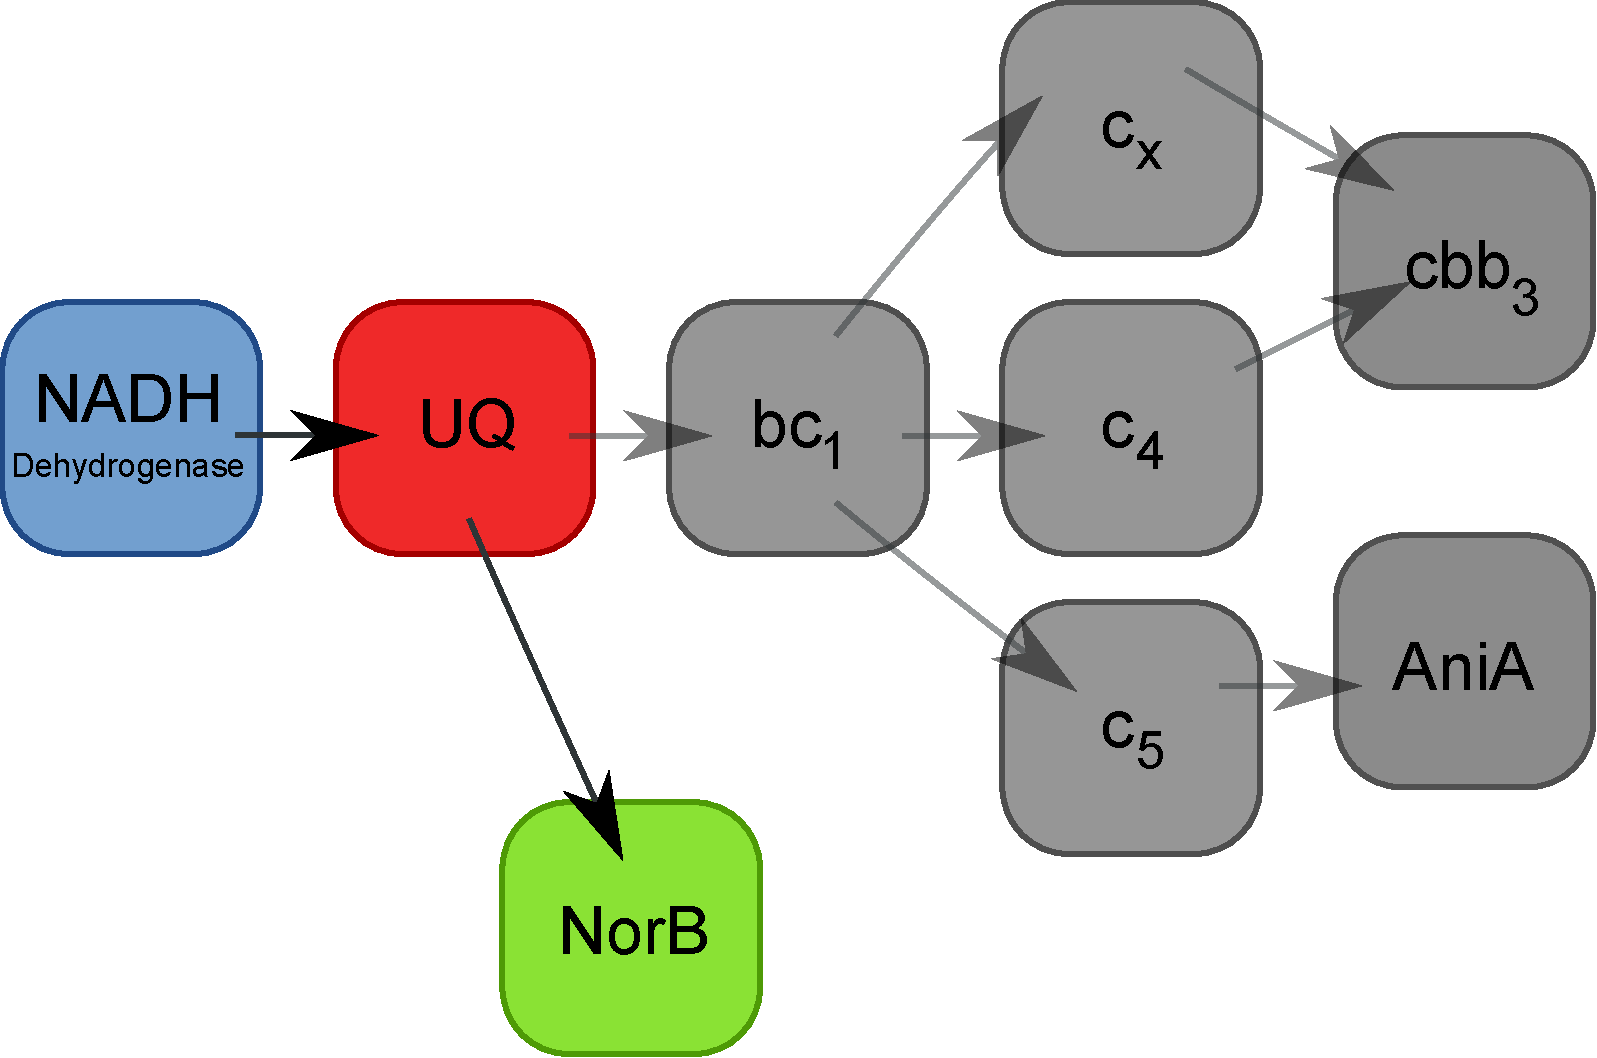
\includegraphics[width=14cm]{06-noreduction/data/no_resp_chain.pdf}
    \caption[Nitric oxide reducing electron transport chain of \Nm{}]{{\bf Nitric oxide reducing electron transport chain of \Nm{}.} This shows the complete electron transport chain of \Nsm{} with the components irrelevant to nitric oxide reduction greyed out.
  \label{fig:no_resp_chain}}
\end{figure}
The equations that describe this portion of the ETC are:
\begin{eqnarray*}
\frac{d[O_2]}{dt} & = & \beta(1-[O_2]/K_O) - k_{1}[C_a][O_2]\\
\frac{d[Q_a]}{dt} & = & g([Q] - [Q_a]) - l_3[Q_a]([B] - [B_a]) - f[Q_a]([X]-[E])\\
\frac{d[E]}{dt} & = & -k_3([C] - [C_a] - [C_X])[E]  - m_3([A] - [A_a])[E] + f[Q_a]([X]-[E])\\
\frac{d[C_a]}{dt} & = & k_3([C] - [C_a] - [C_X])[E] - k_{1}[C_a][O_2] - k_5[C_a][NO]\\
\frac{d[NO]}{dt} & = & m_{1}[NO_2^-][A_a] - l_1[NO][B_a] - k_5[C_a][NO] + k_6 [C_X] - \gamma[NO]\\
\frac{d[C_X]}{dt} & = & k_5[C_a][NO] - k_6 [C_X]\\
\frac{d[B_a]}{dt} & = & l_3[Q_a]([B] - [B_a]) - l_1[NO][B_a]
\end{eqnarray*}
These equations describe the change in concentration of Nitric Oxide over time, which is the experimentally observable value (in addition to the afore modelled oxygen). Also being modelled was the change in concentration of inhibited \cbbthree{} and the reduction state of NorB. This portion of the model involved 24 parameters and variables which I needed to estimate. This number includes the 13 values already estimated in Chapter \ref{chap:oxygenreduction}.
\subsection{Experimental Results}
Generation of nitric oxygen reduction datasets required the growth of MC58 (wild type \Nsm{}) in aerobic conditions until mid log-phase growth had been achieved. This corresponds to an $OD_{600}$ of 0.3-0.9 and usually required an incubation period of roughly 3 hours. Once the required cell density had been obtained, I transferred the culture to the oxygen electrode chamber and recorded the oxygen and nitric oxide concentrations as the culture respired. To model nitric oxide reduction required that I add nitric oxide solution to the culture while it is respiring aerobically. Part-way through aerobic respiration I added nitric oxide solution to various final concentrations at $\approx 5~\mu$M and the culture then left to respire nitric oxide. An example dataset showing the effect of addition of nitric oxide to an aerobically respiring culture is shown in Figures \ref{fig:nodata}, \ref{fig:nodata1} \& \ref{fig:nodata2}.

\begin{figure}[tbp]
 \centering
 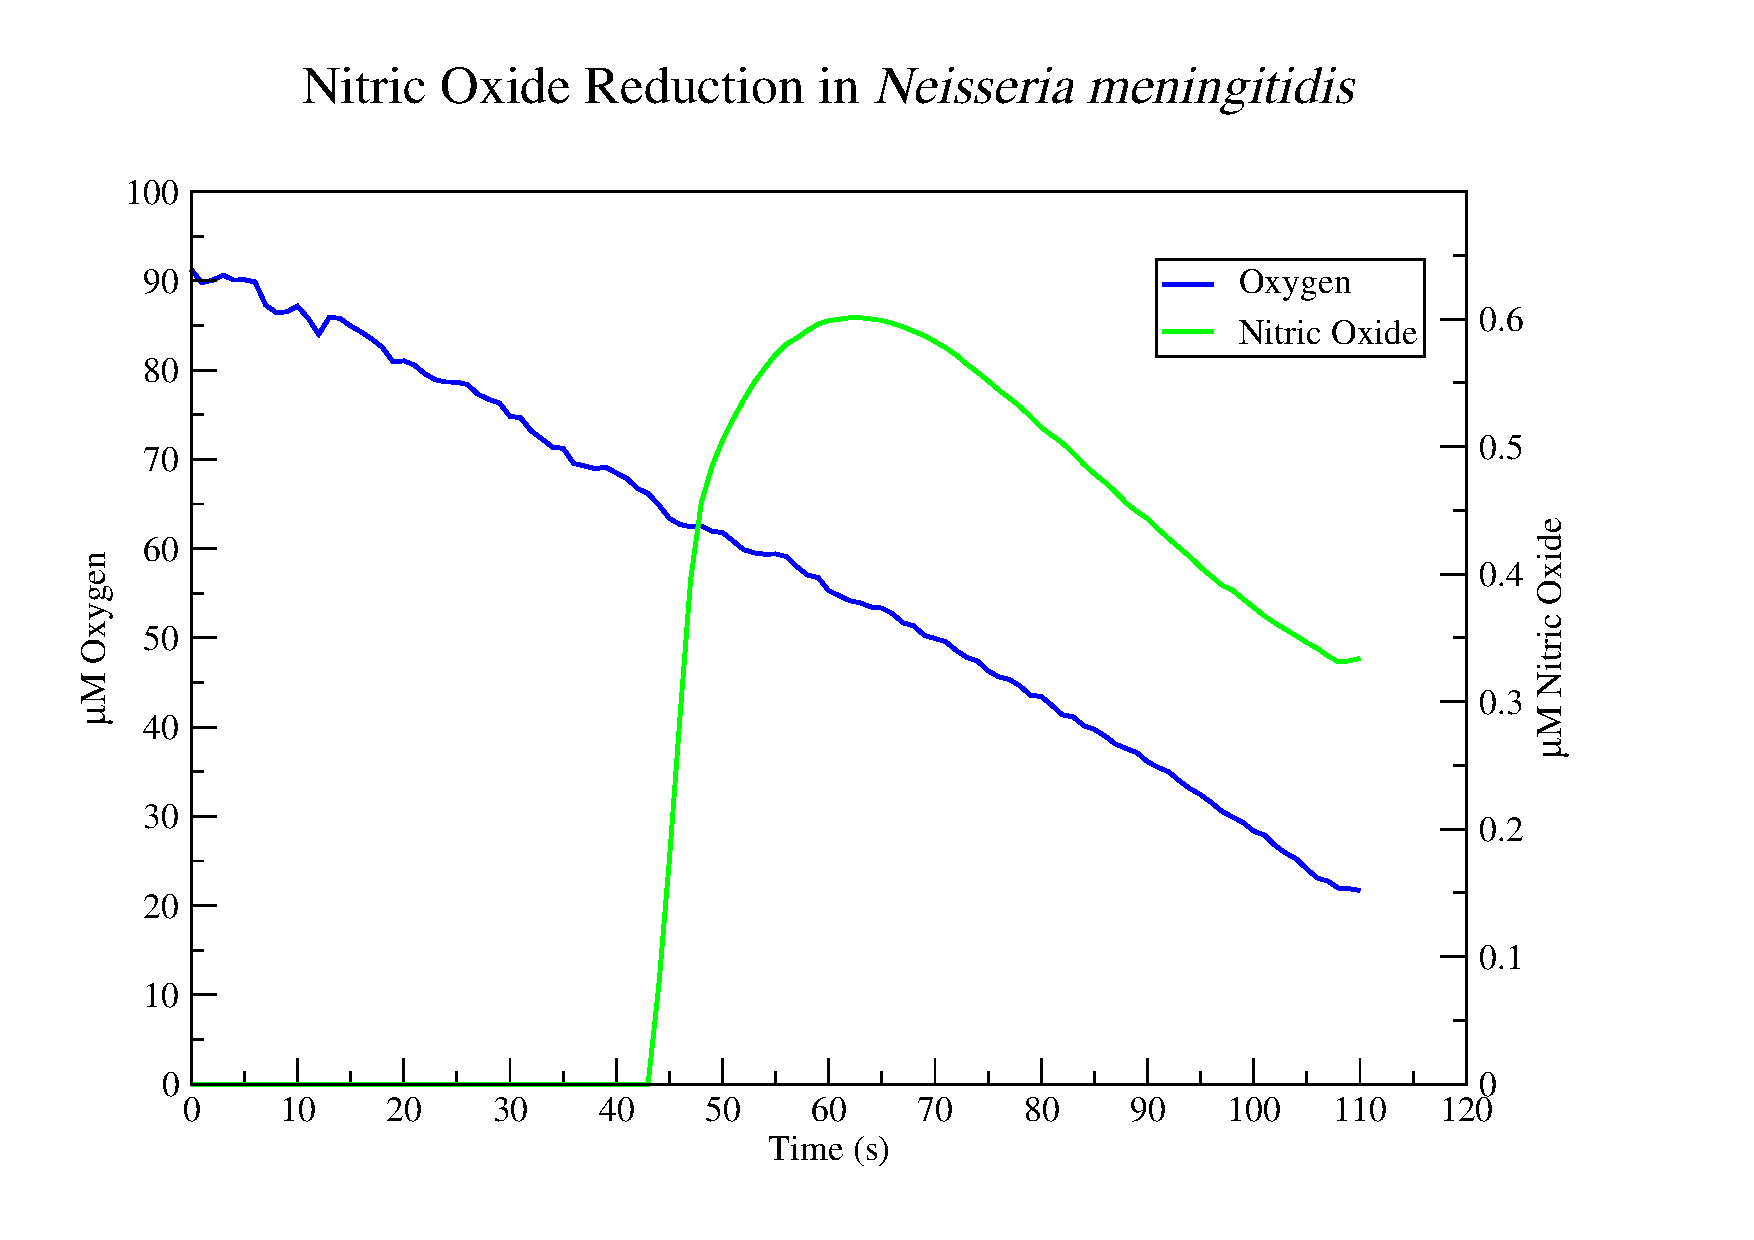
\includegraphics[height=10cm, trim=2cm 1cm 4cm 1cm]{./06-noreduction/data/aer-no-data1.pdf}
 % nosim.eps: 0x0 pixel, 300dpi, 0.00x0.00 cm, bb=0 0 794 595
 \caption[{Nitric Oxide Reduction in \textit{Neisseria meningitidis}.}]{{\bf Nitric Oxide Reduction in \textit{Neisseria meningitidis}.} This dataset shows the effect on rate of oxygen reduction as a small amount of nitric oxide is introduced to the system.}
 \label{fig:nodata1}
\end{figure}
The dataset in Figure \ref{fig:nodata1} shows very little change in the rate of oxygen reduction (it is in fact somewhere around a 3\% reduction in rate) when a small amount of nitric oxide is added. The observed removal of nitric oxide is due primarily to diffusion although there may also be some preliminary (as the culture has not been primed with nitric oxide) nitric oxide reductase activity.

\begin{figure}[tbp]
 \centering
 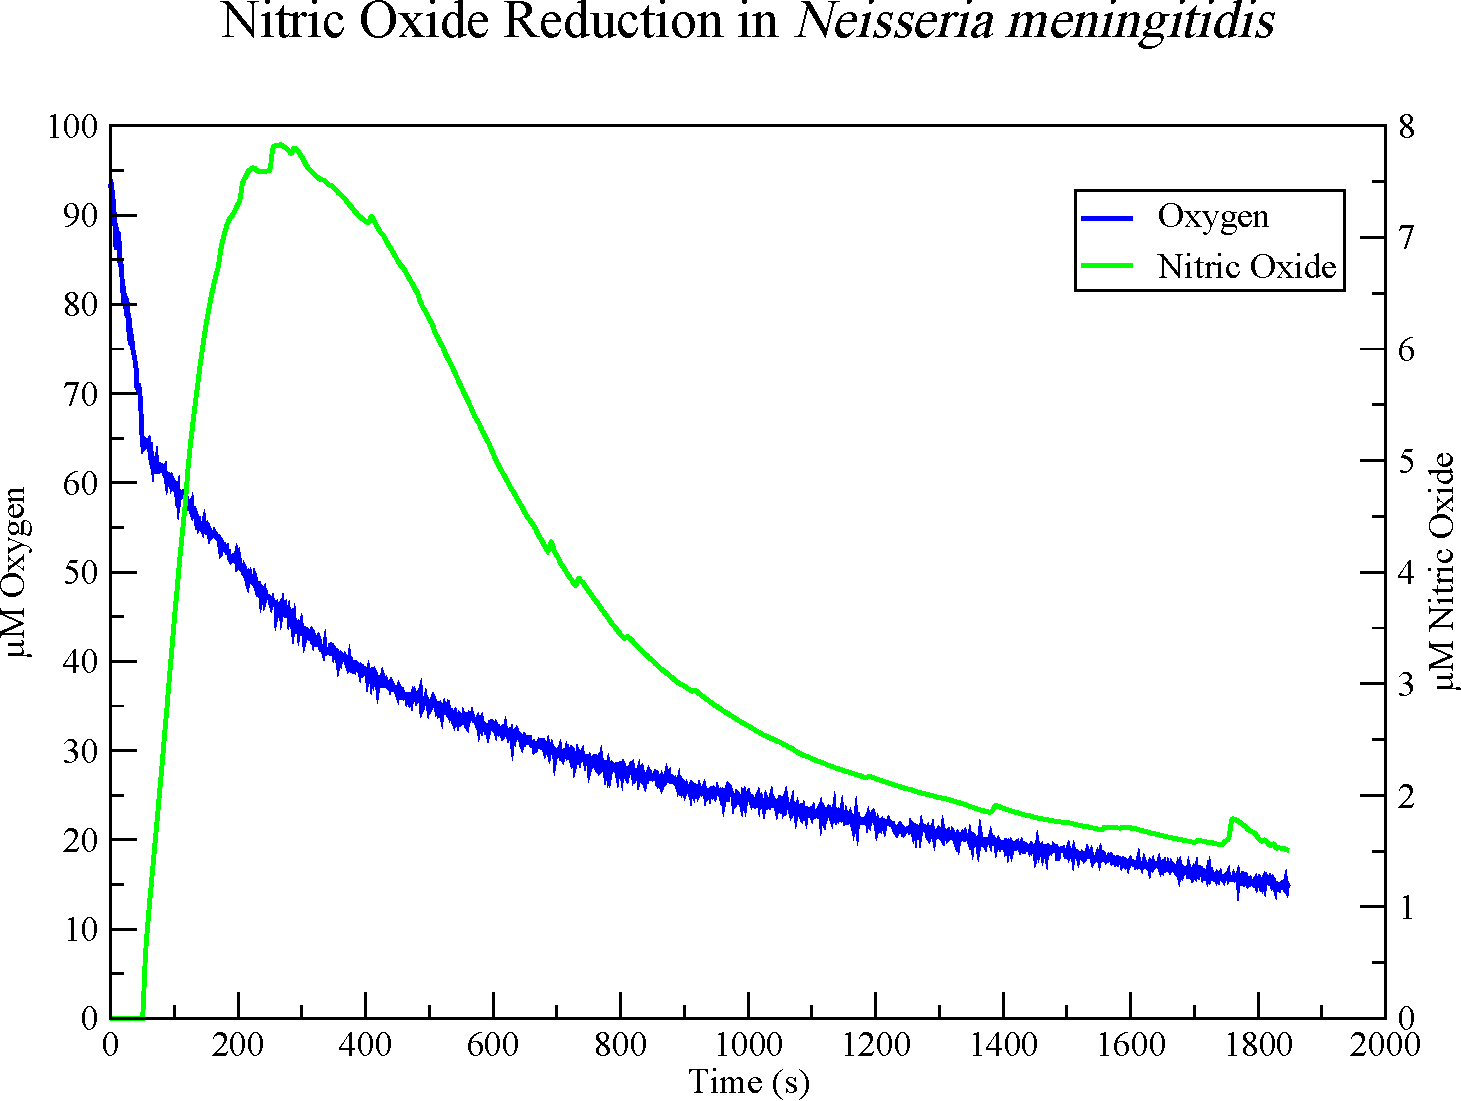
\includegraphics[height=10cm, trim=2cm 1cm 4cm 1cm]{./06-noreduction/data/aer-no-data2.pdf}
 % nosim.eps: 0x0 pixel, 300dpi, 0.00x0.00 cm, bb=0 0 794 595
 \caption[{Nitric Oxide Reduction in \textit{Neisseria meningitidis}.}]{{\bf Nitric Oxide Reduction in \textit{Neisseria meningitidis}.} This dataset shows the effect on rate of oxygen reduction as a larger amount of nitric oxide is introduced to the system.}
 \label{fig:nodata2}
\end{figure}
The dataset in Figure \ref{fig:nodata2} shows a larger change in the rate of oxygen reduction than that of Figure \ref{fig:nodata1} when a larger amount of nitric oxide is introduced. Again the removal of nitric oxide will primarily be due to diffusion, although now at higher concentrations more nitric oxide will interact with \cbbthree{} temporarily inhibiting it. This inhibition causes the reduction in oxidase activity, and the sequestering of NO by \cbbthree{} also causes some of the visible reduction in nitric oxide concentration. The timescale over which the nitric oxide disappears strongly suggests that it is not due to nitric oxide reductase activity. It may also be possible that at this concentration of nitric oxide some \cbbthree{} may have been permanently inhibited as mentioned in Chapters \ref{chap:intro} \& \ref{chap:model}.

\begin{figure}[tbp]
 \centering
 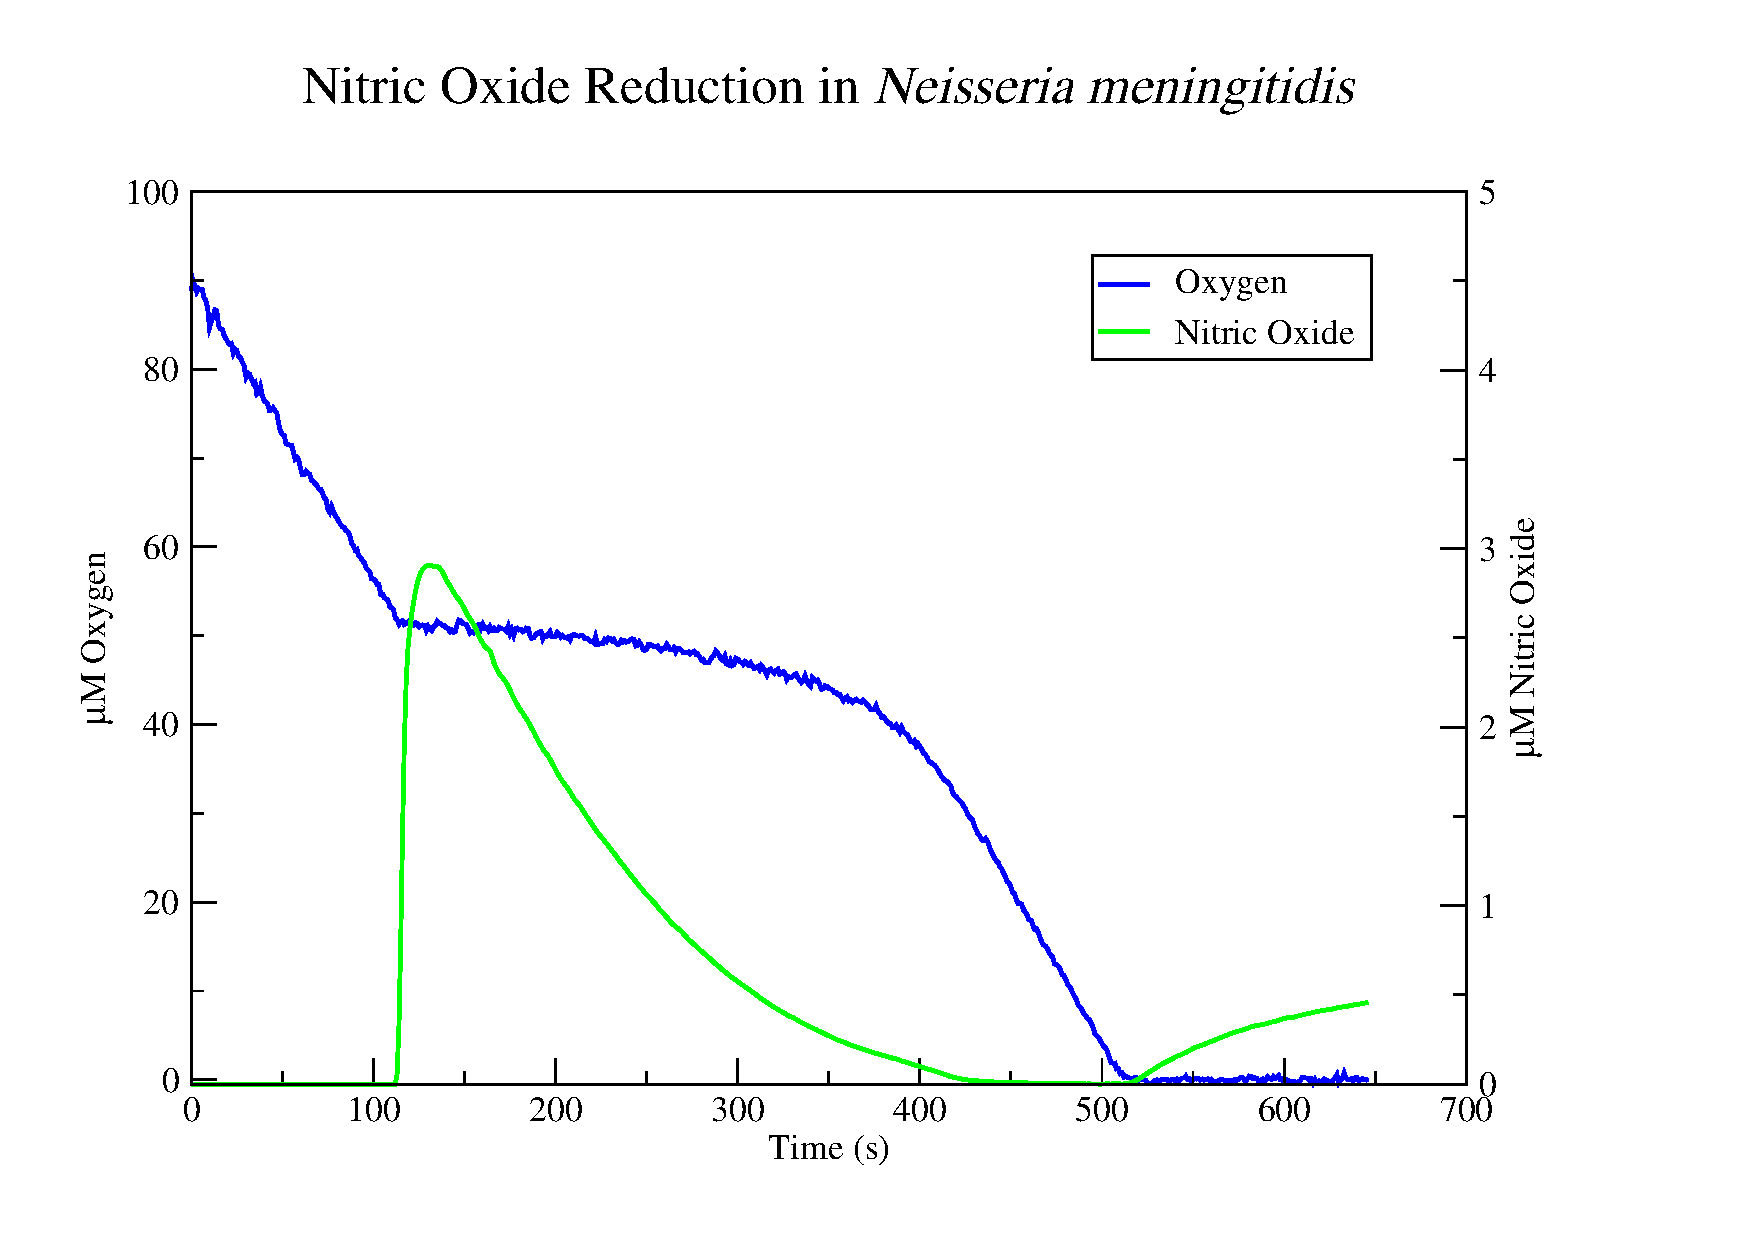
\includegraphics[height=10cm, trim=2cm 1cm 4cm 1cm]{./06-noreduction/data/aer-no-data.pdf}
 % nosim.eps: 0x0 pixel, 300dpi, 0.00x0.00 cm, bb=0 0 794 595
 \caption[{Nitric Oxide Reduction in \textit{Neisseria meningitidis}.}]{{\bf Nitric Oxide Reduction in \textit{Neisseria meningitidis}.} This dataset shows the effect on rate of oxygen reduction as nitric oxide is introduced to the system which appears to have been primed for nitric oxide reduction.}
 \label{fig:nodata}
\end{figure}
The dataset in Figure \ref{fig:nodata} appears to show a system that is partially primed for microaerobic respiration. In this case there is a small amount of NorB (nitric oxide reductase) present. Initially the oxygen reduction is carried out in exactly the same manner as in Chapter \ref{chap:oxygenreduction}. Upon addition of nitric oxide, oxygen respiration slows and almost stops as a result of competition for electrons between \cbbthree{} and NorB, and the direct chemical inhibition of \cbbthree{} by NO. Nitric oxide starts being removed as a combination of diffusion (although this rate will be low as shown in the previous two datasets) and reduction via NorB. Once the NO has been removed from the system oxygen reduction resumes at almost the same rate as before and still has the same high affinity feature as the oxygen reduction datasets in Chapter \ref{chap:oxygenreduction}.
\subsubsection{Prior Probability Distributions}
The prior probability distributions used for parameter estimation of these datasets were a combination of the posterior distributions generated in Chapter \ref{chap:oxygenreduction} and those from the literature as described in Chapter \ref{chap:model}. Where the probability distributions were not generated from the oxygen reduction datasets they were created using them same scheme as described in Chapter \ref{chap:oxygenreduction}. The initial probability distributions used to start the Monte-Carlo runs are shown in Figure \ref{fig:aer_no_priors}. As can be seen, much more information is now available than was present for oxygen reduction.
\begin{figure}[tbp]
 \centering
 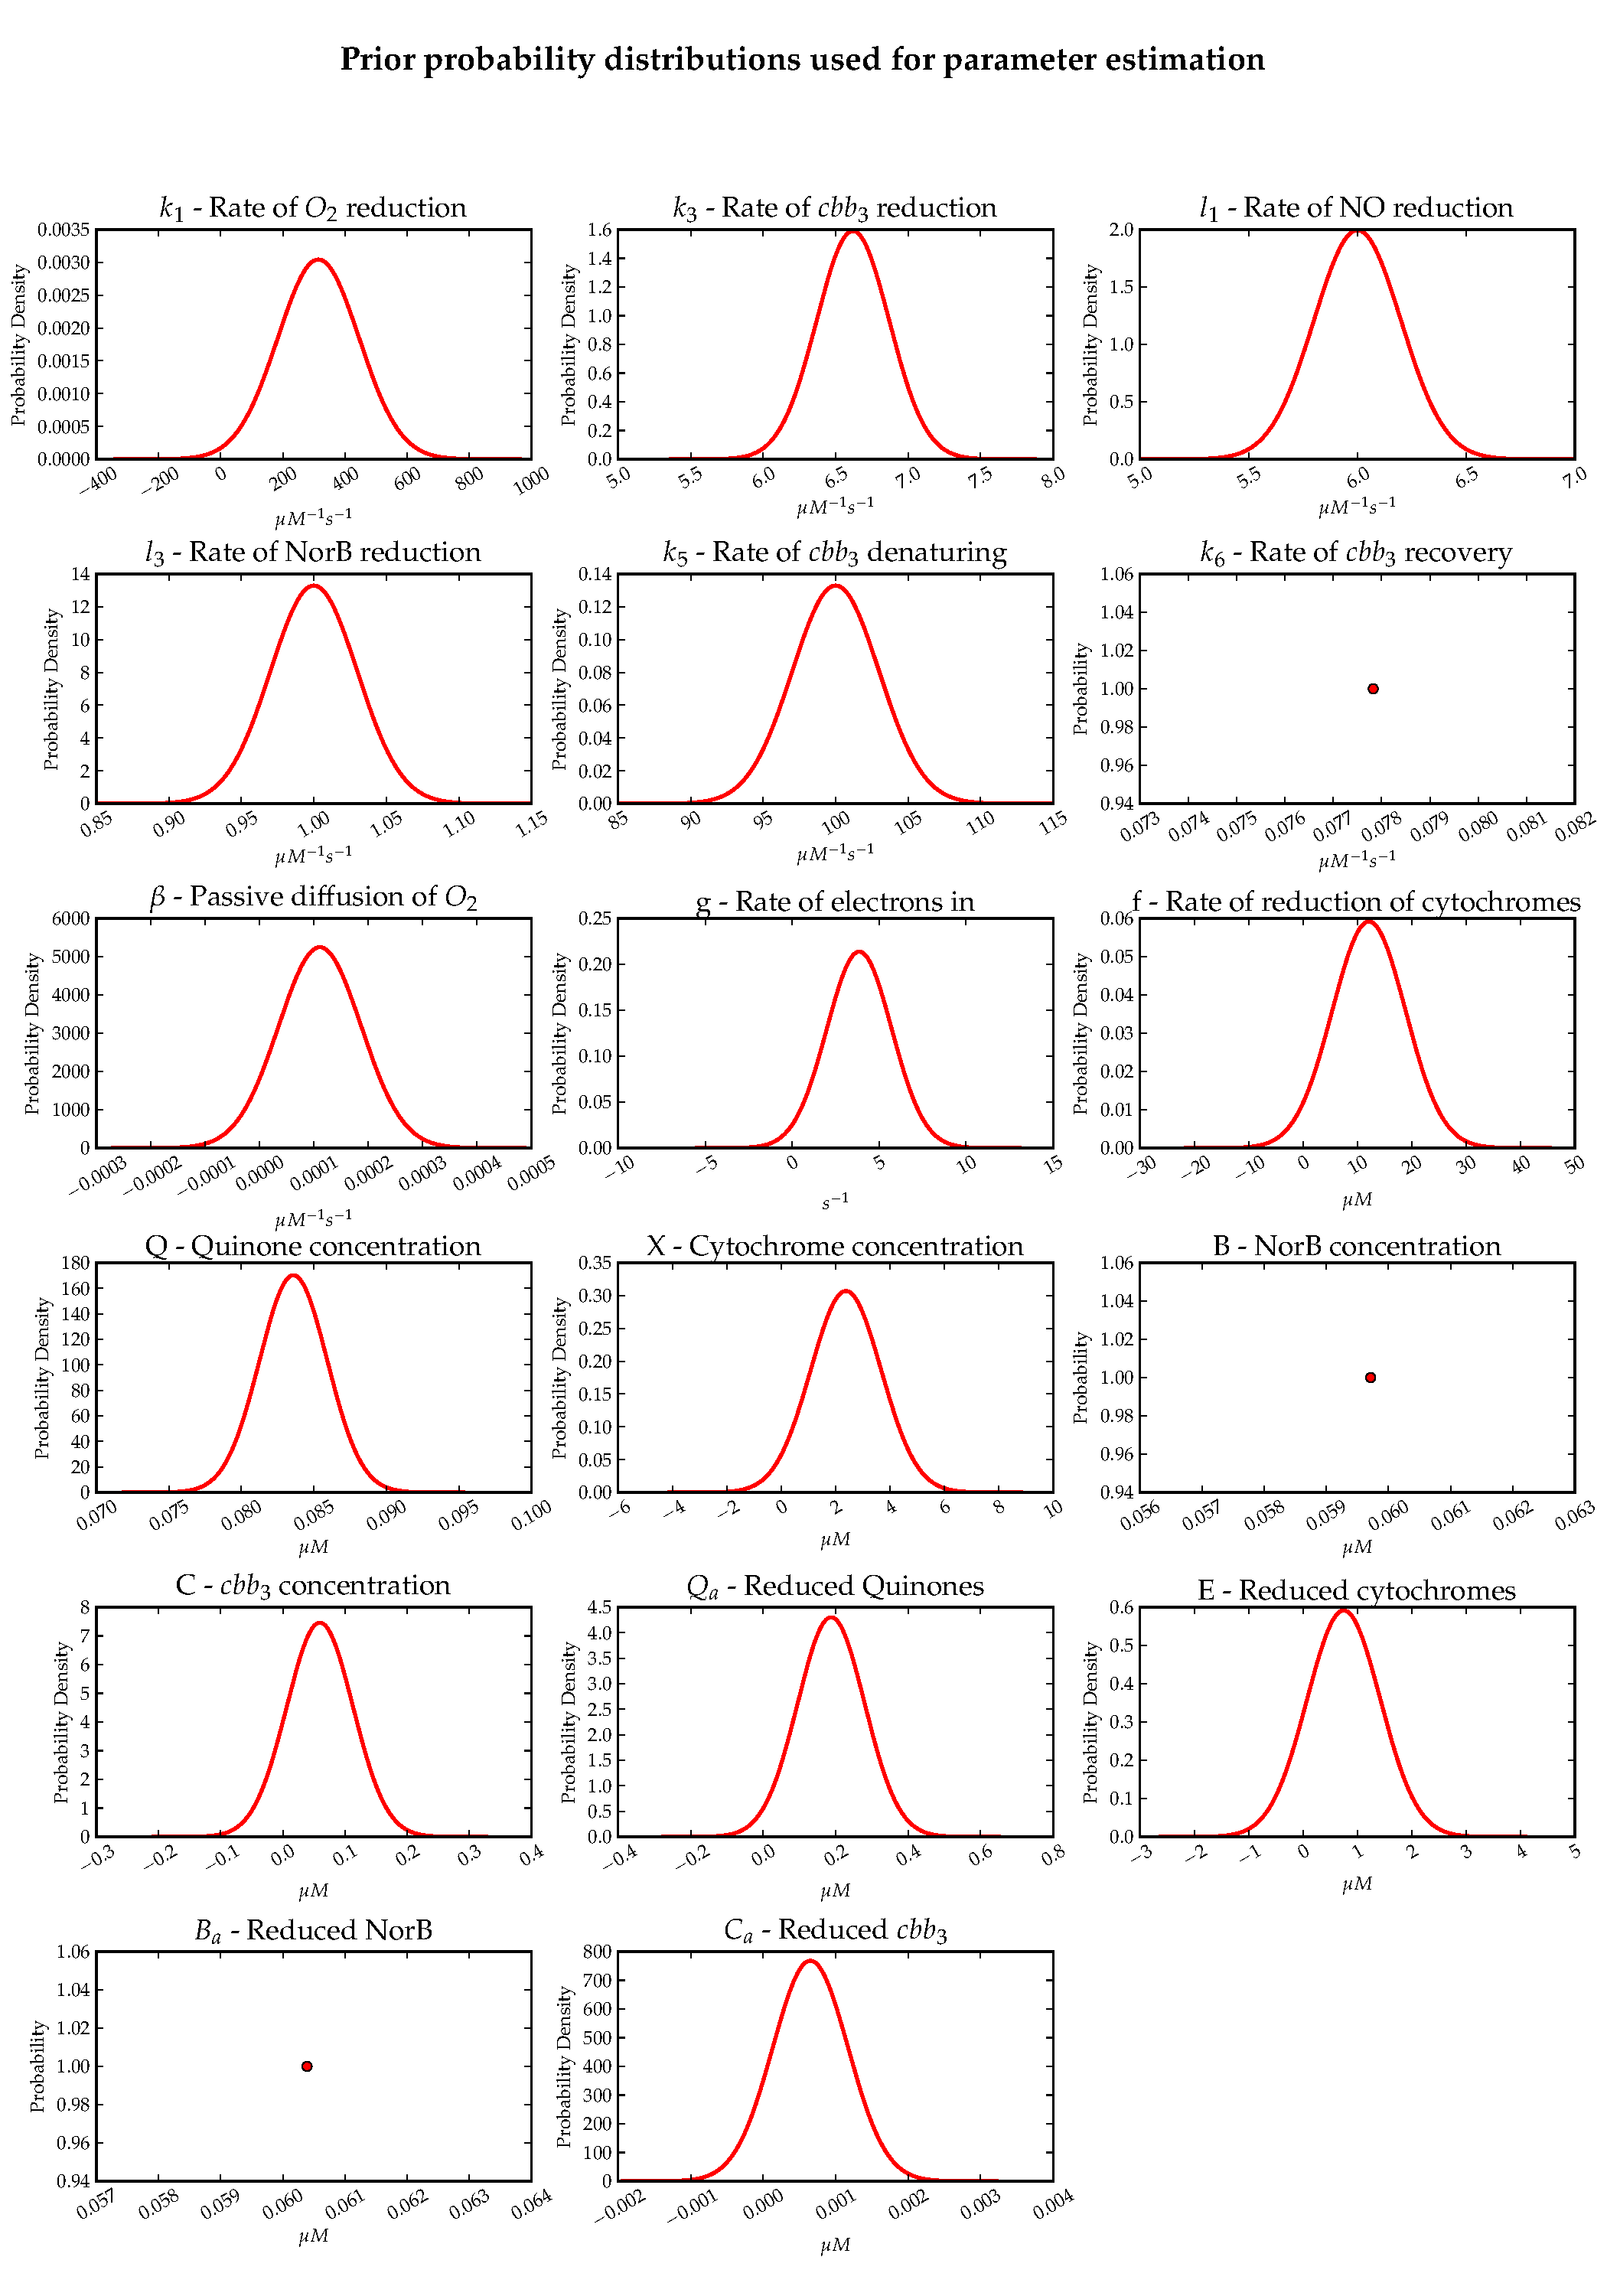
\includegraphics[width=15cm, trim=0cm 0cm 0cm 0cm]{./06-noreduction/data/aer-no-priors.pdf}
 % priors.pdf: 1008x1008 pixel, 72dpi, 35.56x35.56 cm, bb=0 0 1008 1008
 \caption[Prior probability distributions for aerobic nitric oxide reduction]{{\bf Prior probability distributions for aerobic nitric oxide reduction}. These are the probability distributions used as priors by the parameter estimation algorithm. Where no values were available in the literature, the probability distribution represents a flat prior from 0 to $\infty$ with the initial value being determined by preliminary experiment.
 \label{fig:aer_no_priors}}
\end{figure}

\subsubsection{Parameter Estimation Results}
The dataset and final solved output from the Monte-Carlo run are show in Figure \ref{fig:nosim}.  The closeness of fit of the solved parameter set to the experimental data shows that the model has been able to accommodate a parameter set from the prior distributions that is able to accommodate all these features, and will still be able to model simple oxygen reduction.
\begin{figure}[tbp]
 \centering
 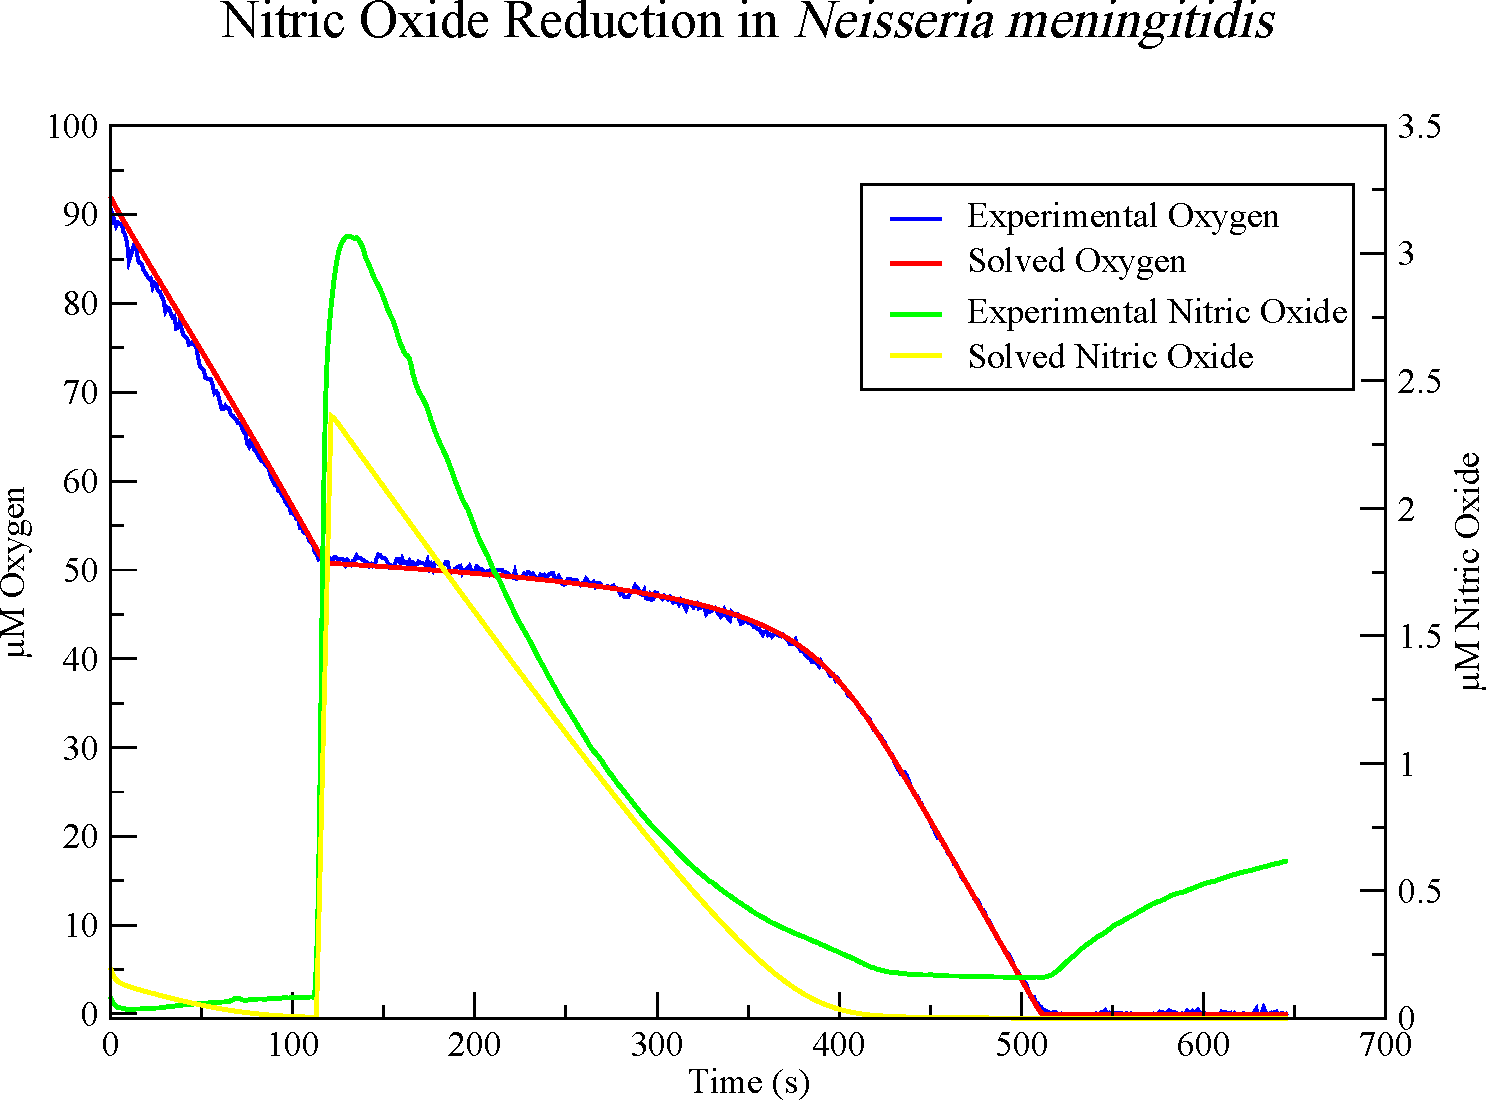
\includegraphics[width=14cm, trim=2cm 1cm 4cm 1cm]{./06-noreduction/data/aer-no-sim.pdf}
 % nosim.eps: 0x0 pixel, 300dpi, 0.00x0.00 cm, bb=0 0 794 595
 \caption[{Nitric Oxide Reduction in \textit{Neisseria meningitidis}.}]{{\bf Nitric Oxide Reduction in \textit{Neisseria meningitidis}.} This dataset shows the effect on rate of oxygen reduction as nitric oxide is introduced to the system. The solved output, using prior probabilities from the oxygen reduction dataset show an almost perfect match to the features of the experimental dataset. The solved oxygen concentrations match the experimental dataset so closely as to be almost invisible.}
 \label{fig:nosim}
\end{figure}
\subsubsection{Analysis of Convergence}
\subsubsection{Analysis of Correlation}
\subsection{Discussion}
\section{Microaerobic Nitric Oxide Reduction}
\subsection{Introduction}
\subsection{Results}
\subsection{Discussion}
\section{\texorpdfstring{Aerobic Nitric Oxide Reduction in \textit{nsrR$^\textrm{-}$} mutant}{Aerobic Nitric Oxide Reduction in nsrR- mutant}}
\subsection{Introduction}
 The $\mathit{nsrR}^-$ mutant, which expresses NorB in an essentially constitutive manner was not effective in generating a usable dataset as it removed any NO almost instantaneously resulting in an almost featureless dataset (data not shown).
\subsection{Results}
\subsection{Discussion}
\chapter{Nitrite Reduction in \Nm{}}

Modelling nitrite reduction involves growing NsrR deficient cultures in aerobic conditions. This mutant expresses AniA and NorB in a constitutive manner, removing the necessity for growing the cultures in microaerobic conditions. The cultures are grown for 3-4 hours after which the culture is added to the electrode chamber and Sodium Nitrite added to a concentration of 1mM.

In the model, Equations (\ref{eq:nitrite} \& \ref{eq:active_ania}) are now also involved, allowing parametrisation of kinetic rates of AniA. This experimental dataset does not unfortunately describe how the concentration of NO changes while Nitrite is being reduced. The prior probability distributions used for this dataset were the posteriors generated from the Nitric Oxide Reduction dataset described above, in accordance with Bayesian inference. The unknown parameters were given non-zero values with flat priors, allowed to burn-in and were then used to generate posterior probability distributions.

A representative dataset and solved output is shown in figure \ref{fig:no2sim}. 

\begin{figure}[ht!]
 \centering
 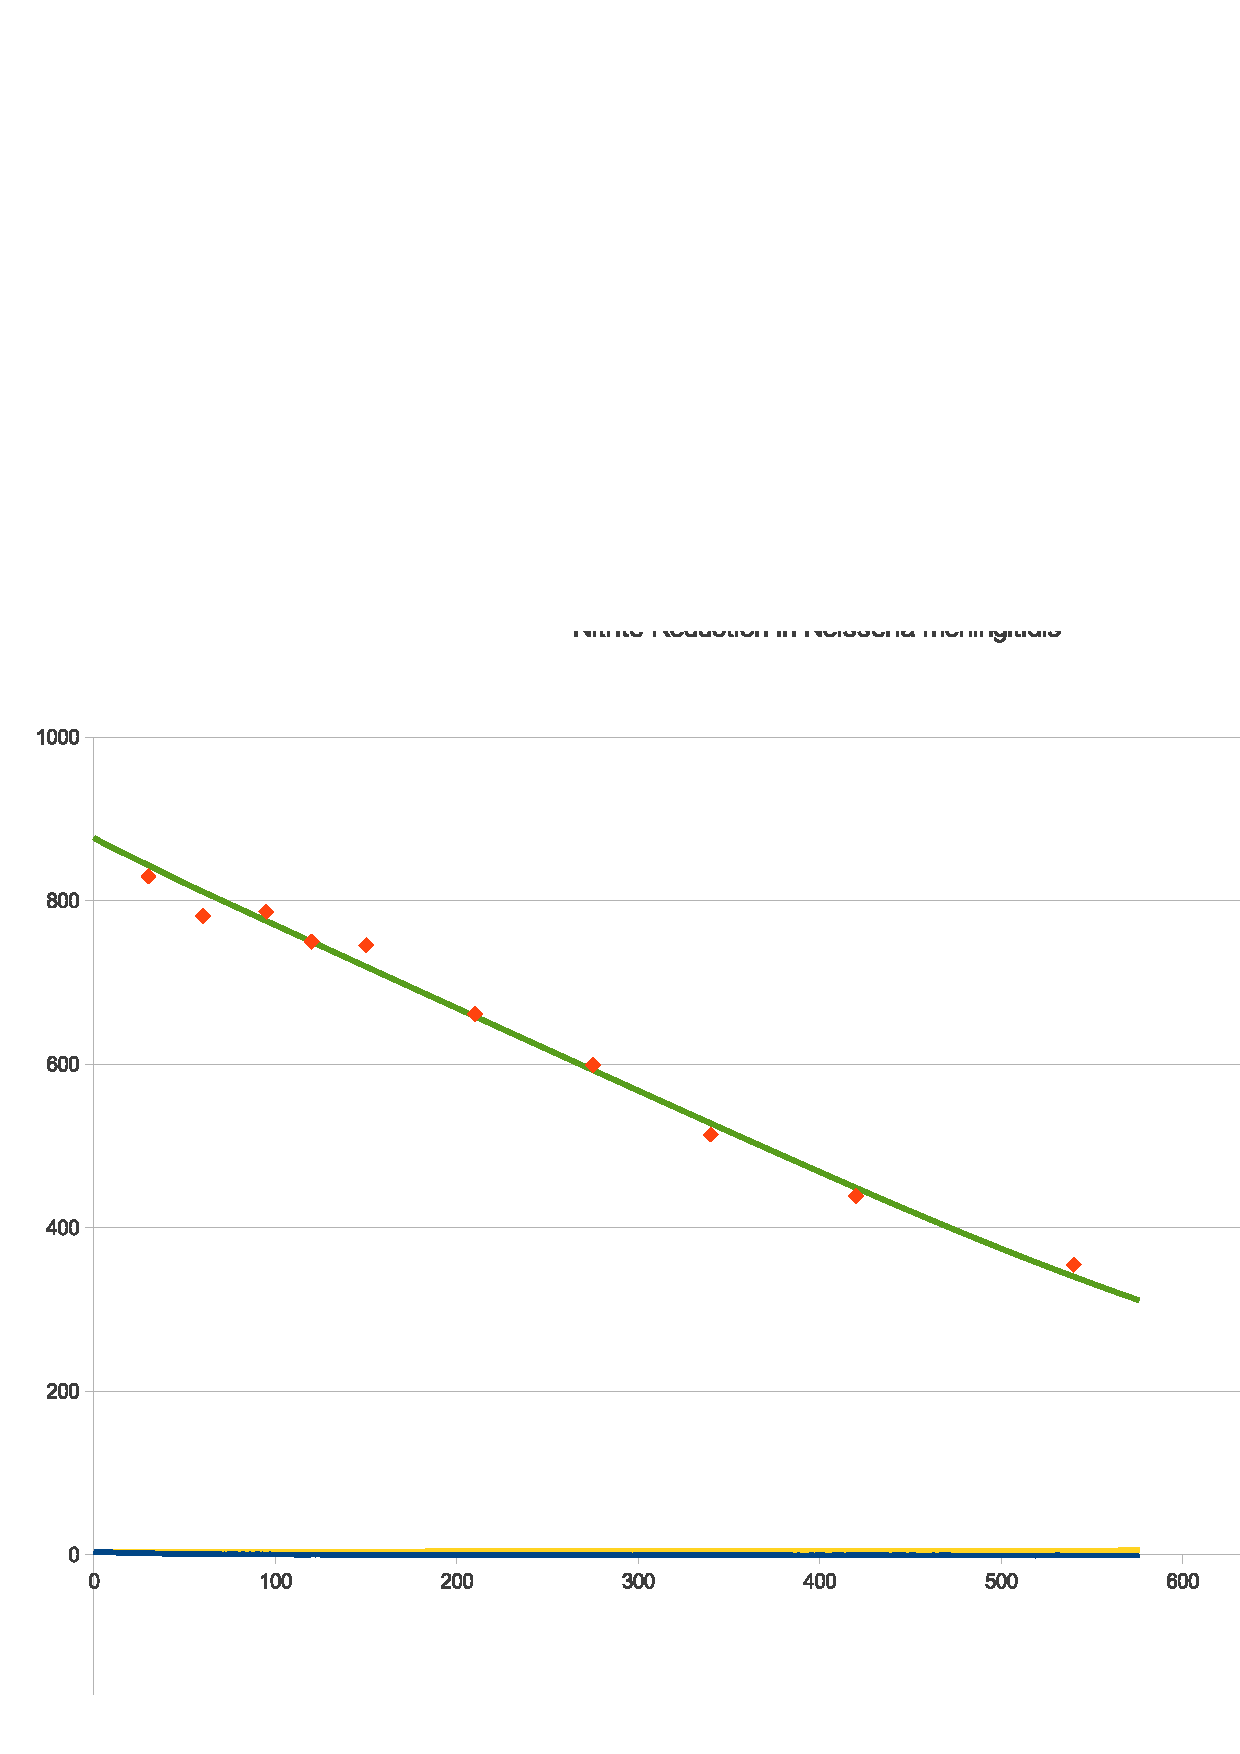
\includegraphics[width=4in]{./07-nitritereduction/data/no2sim.pdf}
 % no2sim.eps: 0x0 pixel, 300dpi, 0.00x0.00 cm, bb=0 0 785 539
 \caption{{\textbf Nitrite Reduction in \textit{Neisseria meningitidis}.} This dataset shows the rate of nitrite reduction when cultures have been grown in microaerobic conditions. The concentrations of nitrite were measured offline leading to discontinuous data, however the solved output closely matches the experimental data for nitrite.}
 \label{fig:no2sim}
\end{figure}

This is a simpler dataset than for Nitric oxide reduction as it only describes nitrite reduction, along with a small change in oxygen concentration. In combination with prior probability distributions from the afore mentioned dataset it means that the possible values for the kinetic rates involved are automatically going to be limited to those that work alongside the given priors. Without the prior probability distributions the posterior distributions would have a similar outcome to that of the first dataset used, where simple oxygen reduction was modelled, i.e. very wide distributions.

%In the case of this dataset, nitrite reduction has been modelled very well, but nitric oxide (and to a small extent, oxygen) has not been [Caveat, this may change when the cluster does eventually spit out the complete trajectory. This then could be moved into the discussion about why priors are important]. Not shown in Figure \ref{fig:no2sim} is the concentration of nitric oxide as nitrite is reduced. Unfortunately the parameter set used to generate the solved output assigned a very low value to the concentration of NorB (even though this should have been being expressed), thus the nitric oxide produced by reduction of nitrite does not itself get reduced, and towards the end of the dataset would be lethal to the culture. In this case, a different prior distribution should have been used for NorB concentration, as it was known beforehand that NorB concentration would be non-zero. This is an example of why the prior distributions are important.

\section{Microerobic Nitrite Reduction}
\subsection{Introduction}
\subsection{Results}
\subsection{Discussion}
\section{Microaerobic Nitrite Reduction in \textit{norB$^\textrm{-}$} mutant}
\subsection{Introduction}
\subsection{Results}
\subsection{Discussion}
\section{Aerobic Nitrite Reduction in \textit{nsrR$^\textrm{-}$} mutant}
\subsection{Introduction}
\subsection{Results}
\subsection{Discussion}
\section{Aerobic Nitrite Reduction in \textit{nsrR$^\textrm{-}$-norB$^\textrm{-}$} mutant}
\subsection{Introduction}
\subsection{Results}
\subsection{Discussion}
\chapter{AniA and NorB expression in \Nm{}}
\section{Aerobic and Microaerobic Expression}
\subsection{Introduction}
\subsection{Results}
\subsection{Discussion}
\svnid{$Id$}
\chapter{Discussion and Completed Model}
\label{chap:completedmodel}
%Therefore I have integrated microbiological techniques with mathematical modelling principles to allow us to understand the system in a way previously not possible. I have constructed a mathematical model which describes \Nsm{} respiration \textit{in silico} and can produce predictions for the system \textit{in vivo}. To parameterise this model I used a novel integrative scheme where a standard Bayesian fitting methodology is interleaved with iterative experimental data collection on progressively more complex respiratory scenarios.
From Chapter \ref{chap:intro}, the stated aims of this thesis were:
\begin{enumerate}
\item {\bf Construct a mathematical model of the \Nm{} respiratory chain.} This will involve the conversion of the kinetic reactions involved in respiration into mathematical equations that can be linked together, and if justified simplifying the chain.
\item {\bf Obtain experimental data on respiratory rates and enzyme kinetics.} This will involve performing experiments on respiring \Nm{} and recording the concentrations of respiratory substrates under different conditions.
\item {\bf Parametrise the model using experimental data.} To do this a system will need to be developed which can iteratively fit experimental data to specific parts of the mathematical model.
\end{enumerate}

\noindent With reference to the above, a mathematical model was constructed as described in Chapter \ref{chap:model}, the equations shown below:
\begin{eqnarray*}
\frac{d[O_2]}{dt} & = & \beta(1-[O_2]/K_O) - k_{1}[C_a][O_2]\\ \nonumber
\frac{d[NO]}{dt} & = & m_{1}[NO_2^-][A_a] - l_1[NO][B_a] - k_5[C_a][NO] + k_6 [C_X] - \gamma[NO]\\ \nonumber
\frac{d[NO_2^-]}{dt} & = & - m_{1}[NO_2^-][A_a]\\ \nonumber
\frac{d[Q_a]}{dt} & = & g([Q] - [Q_a]) - l_3[Q_a]([B] - [B_a]) - f[Q_a]([X]-[X_a])\\ \nonumber
\frac{d[X_a]}{dt} & = & -k_3([C] - [C_a] - [C_X])[X_a]  - m_3([A] - [A_a])[X_a] + f[Q_a]([X]-[X_a])\\ \nonumber
\frac{d[C_a]}{dt} & = & k_3([C] - [C_a] - [C_X])[X_a] - k_{1}[C_a][O_2] - k_5[C_a][NO] + k_6[C_X]\\ \nonumber
\frac{d[C_X]}{dt} & = & k_5[C_a][NO] - k_6 [C_X]\\ \nonumber
\frac{d[A_a]}{dt} & = & m_3([A] - [A_a])[X_a]- m_{1}[NO_2^-][A_a]\\ \nonumber
\frac{d[B_a]}{dt} & = & l_3[Q_a]([B] - [B_a]) - l_1[NO][B_a]
\end{eqnarray*}
Additionally if the preliminary suggested expression equations are to be included this list is extended to include:
\begin{eqnarray*}
\frac{d[A]}{dt} & = & \left(R\left(1 - \frac{[O_2] + k_{10}[NO]}{[O_2] + k_{10}[NO] + k_{11}}\right) - S\left(1 - \frac{[NO]}{[NO] + k_{13}}\right)\right) - k_8[A] \nonumber \\
\frac{d[B]}{dt} & = & T \left(\frac{[NO]}{[NO] + k_{15}}\right) - k_{16}[B]
\end{eqnarray*}

The data required to populate the parameters has been obtained by experimental means as described in Chapters \ref{chap:oxygenreduction}-\ref{chap:nitritereduction}. These data provided information on both respiratory rates and enzyme kinetics. Additional information was gathered from the literature as shown in Chapter \ref{chap:model}.

To use the information obtained from the literature and from experimental data, an integrated parameter estimation scheme was devised, which combined Bayesian inference with a Monte-Carlo type parameter estimation system into an iterative method for extracting parameter values from progressively more complex datasets as described in Chapter \ref{chap:paramest}. This iterative method produces posterior probability distributions for each of the parameters in the model calculated from the various rounds of parameter estimation for each successive dataset. The final parameter probability distributions are shown in tabular form in Table \ref{tab:final_parameters}. This table shows the values required to produce idealised lognormal distributions of each of the parameters. Plots of the actual obtained distributions are shown in Figure \ref{fig:final_posteriors}.
\begin{table}[tbp]
\begin{center}
\begin{tabular}{>{\centering}m{1.4cm}>{\centering}m{6.1cm}>{\centering}m{2.7cm}>{\centering}m{2.5cm}}
\toprule
\textbf{Symbol} & \textbf{Description} & \textbf{Mean Value} & \textbf{$\sigma$}
\tabularnewline
\midrule
$k_1$ & Rate constant for O$_{\textrm{2}}$ reduction by reduced \cbbthree{} & $403.51~\mu M^{-1} s^{-1}$ & $27.59$
\tabularnewline\noalign{\smallskip}\hline\noalign{\smallskip}

$k_3$ & Rate constant for \cbbthree{} reduction by cytochrome pool & $4.58~\mu M^{-1} s^{-1}$ & $0.436$
\tabularnewline\noalign{\smallskip}\hline\noalign{\smallskip}

$l_1$ & Rate constant for NO reduction by reduced NorB & $6.42~\mu M^{-1} s^{-1}$ & 2.33
\tabularnewline\noalign{\smallskip}\hline\noalign{\smallskip}

$l_3$ & Rate constant for NorB reduction by quinone pool & $0.096~\mu M^{-1} s^{-1}$ & $0.025$
\tabularnewline\noalign{\smallskip}\hline\noalign{\smallskip}

$m_1$ & Rate constant for NO$_{\textrm{2}}^{\textrm{-}}$ reduction by reduced AniA & $0.175~\mu M^{-1} s^{-1}$ & $0.087$
\tabularnewline\noalign{\smallskip}\hline\noalign{\smallskip}

$m_3$ & Rate constant for AniA reduction by cytochrome pool & $4.79~\mu M^{-1}s^{-1}$ & $0.042$
\tabularnewline\noalign{\smallskip}\hline\noalign{\smallskip}

$k_5$ & Rate constant for \cbbthree{} inhibition by NO & $\approx66000~\mu M ^{-1} s ^{-1}$ & Indeterminate
\tabularnewline\noalign{\smallskip}\hline\noalign{\smallskip}

$k_6$ & Rate constant for recovery of NO inhibited \cbbthree{} & $1.59~s^{-1}$ & $0.527$
\tabularnewline\noalign{\smallskip}\hline\noalign{\smallskip}

$\beta$ & Rate constant for passive diffusion in of O$_{\textrm{2}}$ & $0.00014~\mu M^{-1} s^{-1}$ & $4.7\times10^6$
\tabularnewline\noalign{\smallskip}\hline\noalign{\smallskip}

$K_O$ & Saturation O$_{\textrm{2}}$ level & $48~\mu M$ & $0$
\tabularnewline\noalign{\smallskip}\hline\noalign{\smallskip}

$g$ & Rate of electrons in from NADH & $0.085~s^{-1}$ & $0.0078$
\tabularnewline\noalign{\smallskip}\hline\noalign{\smallskip}

$f$ & Rate constant for reduction of cytochromes by quinones & $0.771~\mu M^{-1}s^{-1}$ & $0.096$
\tabularnewline\noalign{\smallskip}\hline\noalign{\smallskip}

$\gamma$ & Spontaneous loss of NO & $0.0024~\mu Ms^{-1}$ & $8.8\times10^5$
\tabularnewline\noalign{\smallskip}\hline\noalign{\smallskip}

$Q$ & Concentration of quinones & $34.31~\mu M$ & $5.49$
\tabularnewline\noalign{\smallskip}\hline\noalign{\smallskip}

$X$ & Concentration of cytochromes & $2.81~\mu M$ & $0.595$
\tabularnewline\noalign{\smallskip}\hline\noalign{\smallskip}

$A$ & Concentration of AniA & $0.704~\mu M$ & $0.3$
\tabularnewline\noalign{\smallskip}\hline\noalign{\smallskip}

$B$ & Concentration of NorB & $7.8~\mu M$ & $3.63$
\tabularnewline\noalign{\smallskip}\hline\noalign{\smallskip}

$C$ & Concentration of \cbbthree{} & $1.3~\mu M$ & $0.259$
\tabularnewline
\bottomrule
\end{tabular}
\caption[Model parameters]{{\bf Model parameters.} This table shows all the parameter values that have been generated by iterative parameter estimation throughout this work. For values that show concentrations of components, they represent the value for a culture with $OD_{600}=1.00$.
\label{tab:final_parameters}}
\end{center}
\end{table}

\begin{figure}[tbp]
 \centering
 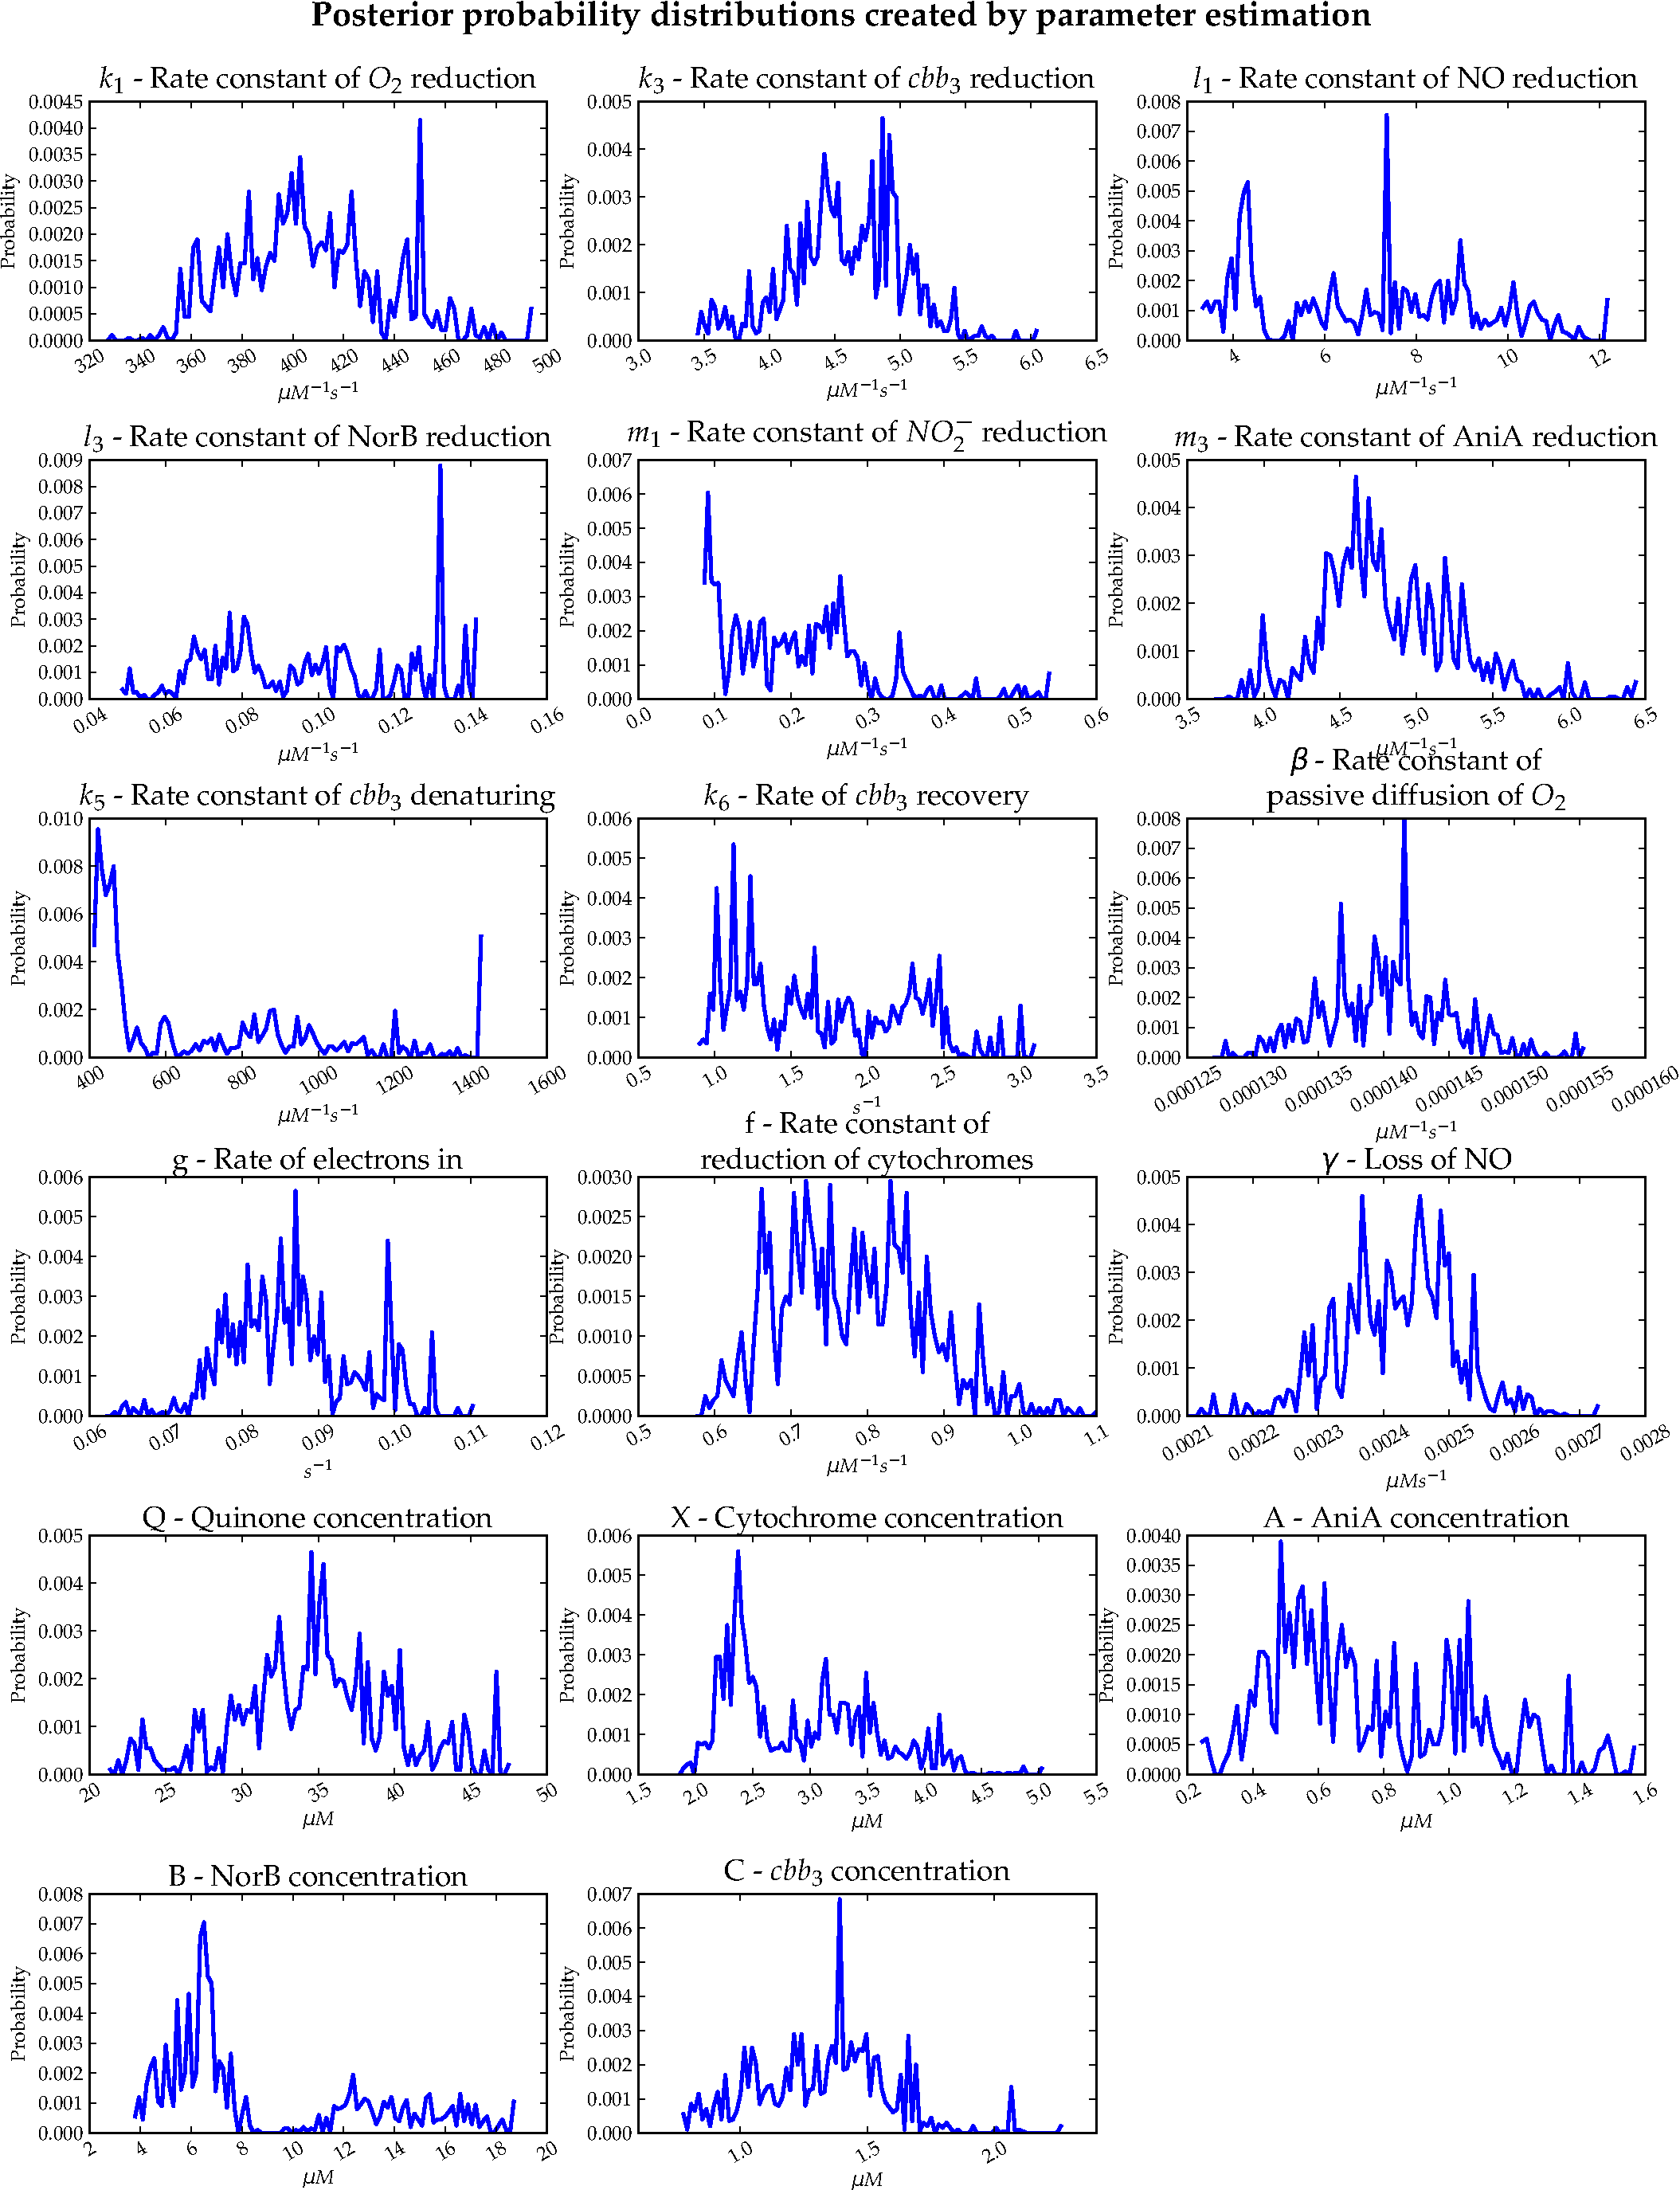
\includegraphics[width=15cm, trim=0cm 0cm 0cm 0cm, clip=true]{./09-completedmodel/data/posteriors.pdf}
 % priors.pdf: 1008x1008 pixel, 72dpi, 35.56x35.56 cm, bb=0 0 1008 1008
 \caption[Final Posterior probability distributions]{{\bf Final Posterior probability distributions}. These are the final posterior probability distributions generated by the parameter estimation system, all concentrations have been normalised to assume an $OD_{600}$ of 1. Note the value of $k_5$ will be significantly different from that shown.
 \label{fig:final_posteriors}}
\end{figure}

The value of $k_5$ has no associated bounds in the table as it was concluded that the value reported is actually much lower than the true value as evidenced in Chapter \ref{chap:nitritereduction} whereby the posterior parameters from nitrite reduction were unable to model the true effect of NO inhibition of oxygen shown in Chapter \ref{chap:noreduction}. Increasing the value of $k_5$ could restore the correct behaviour in the NO reduction dataset without a significant detrimental effect on the nitrite dataset. Unfortunately this makes the bounds on this value indeterminate without further Monte-Carlo simulation being run with the adapted value. The distribution shown in Figure \ref{fig:final_posteriors} shows the un-adapted values for comparison.

\section{Amalgamation of Cytochromes}
The choice to replace the multiple cytochromes $bc_1$, $c_x$, $c_4$ and $c_5$ with one single entity was a modelling one, to both simplify the modelling process by reducing the total component count and number of rate constants, and to allow the model to focus on simple electron transport chain branching and competition for electrons. The rate constants for each of the cytochromes could be subsumed by the respective ``out rates'' from the amalgamated cytochrome to its downstream electron acceptor. The downside of this approach is that it means that any rates obtained for $X$ are probably not going to be biologically relevant as it is essentially masking the behaviour of multiple different hidden components. This simplification does not appear to have affected the model in a detrimental way when using the datasets in this work.

\section{Parameter Changes Throughout this Work}
\begin{table}[tbp]
\begin{center}
\begin{tabular}{ccccc}
\toprule
\textbf{Parameter} & \textbf{Prior} & \textbf{Oxygen Posterior} & \textbf{NO Posterior} & \textbf{Nitrite Posterior}
\tabularnewline
\midrule
$k_1$ & $415$ & $413.228$ & $417.88$ & $403.51$
\tabularnewline\noalign{\smallskip}\hline\noalign{\smallskip}

$k_3$ & $3$ & $4.496$ & $4.65$ & $4.5$
\tabularnewline\noalign{\smallskip}\hline\noalign{\smallskip}

$l_1$ & $6$ & $\rightarrow$ & $13.12$ & $6.42$
\tabularnewline\noalign{\smallskip}\hline\noalign{\smallskip}

$l_3$ & $1$ & $\rightarrow$ & $0.058$ & $0.096$
\tabularnewline\noalign{\smallskip}\hline\noalign{\smallskip}

$m_1$ & $1$ & $\rightarrow$ & $\rightarrow$ & $0.175$
\tabularnewline\noalign{\smallskip}\hline\noalign{\smallskip}

$m_3$ & $4.8$ & $\rightarrow$ & $\rightarrow$ & $4.79$
\tabularnewline\noalign{\smallskip}\hline\noalign{\smallskip}

$k_5$ & $100$ & $\rightarrow$ & $1741.8$ & $66000$
\tabularnewline\noalign{\smallskip}\hline\noalign{\smallskip}

$k_6$ & $38$ & $\rightarrow$ & $1.076$ & $1.59$
\tabularnewline\noalign{\smallskip}\hline\noalign{\smallskip}

$\beta$ & $0.00014$ & $0.00012$ & $0.00014$ & $0.00014$
\tabularnewline\noalign{\smallskip}\hline\noalign{\smallskip}

$g$ & $0.847$ & $0.889$ & $0.857$ & $0.085$
\tabularnewline\noalign{\smallskip}\hline\noalign{\smallskip}

$f$ & $8.749$ & $8.707$ & $8.398$ & $0.771$
\tabularnewline\noalign{\smallskip}\hline\noalign{\smallskip}

$\gamma$ & $0.017$ & $\rightarrow$ & $0.0024$ & $0.0024$
\tabularnewline\noalign{\smallskip}\hline\noalign{\smallskip}

$Q$ & $0.3$ & $3.143$ & $7.06$ & $34.31$
\tabularnewline\noalign{\smallskip}\hline\noalign{\smallskip}

$X$ & $3.97$ & $4.732$ & $27.45$ & $2.81$
\tabularnewline\noalign{\smallskip}\hline\noalign{\smallskip}

$A$ & $0.137$ & $\rightarrow$ & $\rightarrow$ & $0.704$
\tabularnewline\noalign{\smallskip}\hline\noalign{\smallskip}

$B$ & $0.043$ & $\rightarrow$ & $0.137$ & $7.8$
\tabularnewline\noalign{\smallskip}\hline\noalign{\smallskip}

$C$ & $0.03$ & $0.043$ & $0.071$ & $1.3$
\tabularnewline
\bottomrule
\end{tabular}
\caption[Change in Parameter Values]{{\bf Change in Parameter Values.} This table shows the mean of each parameter value at each stage of the model. Where parameters are not used and therefore generate no posterior distribution, a $\rightarrow$ is used instead.
\label{tab:parameter_changes}}
\end{center}
\end{table}

The way the parameters change throughout the various rounds of parameter estimation described in this work is presented in Table \ref{tab:parameter_changes} and discussed below.
\begin{itemize}
\setlength{\itemsep}{0cm}
 \item $k_1$ - Changes very little and the final distribution resembles the prior distribution very closely.
 \item $k_3$ - Increases slightly to achieve the required oxygen reduction rate and affinity.
 \item $l_1$ - Increases by a factor of two initially however this is a very broad distribution suggesting that the magnitude is less important at this point. It settles back to a value closer to the prior when a more appropriate dataset is used.
 \item $l_3$ - Reduces significantly to achieve desired NO reduction rate.
 \item $m_1$ - Reduces significantly to achieve desired nitrite reduction rate.
 \item $m_3$ - Changes very little from prior distribution.
 \item $k_5$ - Increases significantly in order to inhibit \cbbthree{} by the amount seen in experimental data.
 \item $k_6$ - Decreases significantly for the same reason as above.
 \item $\beta$ - No change.
 \item $g$ - No change initially, but final posterior shows a $10\times$ decrease to prevent permanent reduction of cytochromes.
 \item $f$ - No change initially, but final posterior shows a $10\times$ decrease to prevent permanent reduction of quinone pool.
 \item $\gamma$ - Initial decrease to prevent NO being lost too quickly from the \textit{in silico} results.
 \item $Q$ - Initial increase to allow enough electron flux through the system. Final large increase as a result of reducing electron flux \textit{into} the system.
 \item $X$ - Significant change seen for NO reduction, but this change is negated in the final posteriors after reducing electron flux.
 \item $A$ - Significant increase required to attain observed Nitrite reduction rate after reducing electron flux.
 \item $B$ - Increases required to attain Nitric Oxide reduction rate, and after reducing electron flux.
 \item $C$ - Significant increase required to attain Oxygen reduction rate, exacerbated by the reduction of electron flux.
\end{itemize}

\section{Testing the Model}
\subsection{\texorpdfstring{Addition of Nitric Oxide to an \textit{nsrR}$^-$ mutant}{Addition of Nitric Oxide to an nsrR- mutant}}
The $nsrR^-$ mutant should express NorB at significantly higher levels than in wild-type cultures, by as much as $100\times$ according to \citet{Rock2007}. This is a simple \textit{in silico} test to do as it simply requires the concentration of NorB to be increased by $100\times$. Additionally a representative experimental dataset which has not been used during parameter estimation can be used to compare the \textit{in silico} result with the \textit{in vivo} data. This experimental dataset is shown in Figure \ref{fig:aniAnsrR} and repeated here in Figure \ref{fig:aniAnsrR1}.
\begin{figure}[tbp]
 \centering
 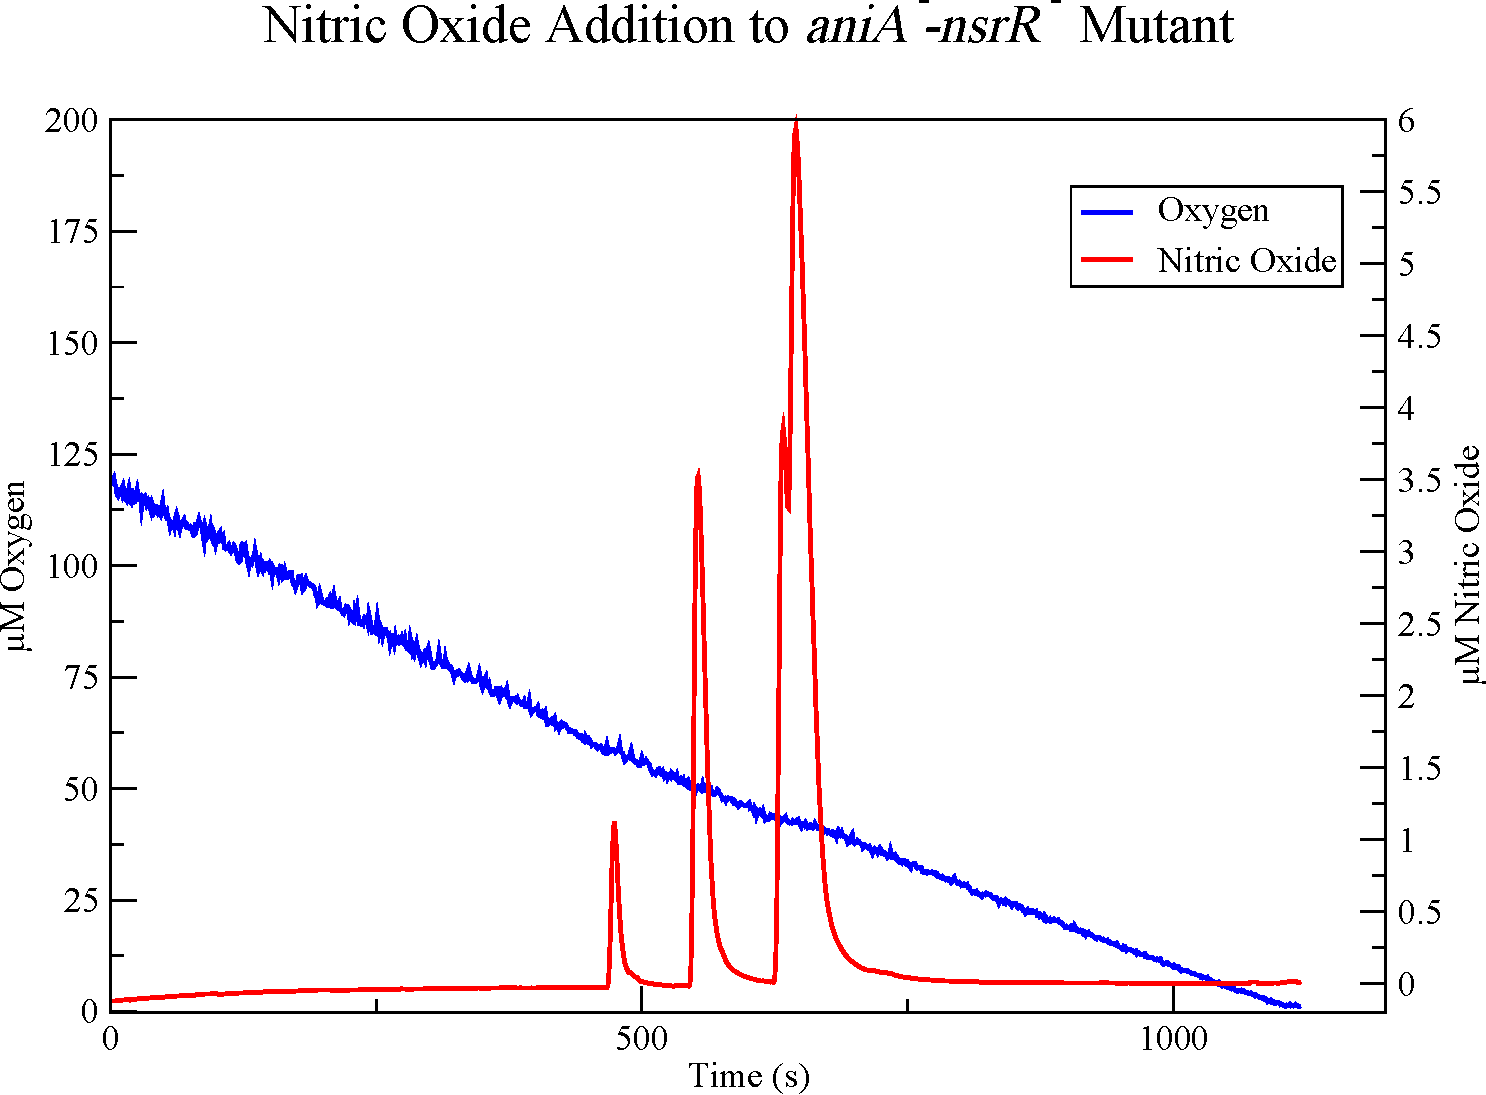
\includegraphics[width=15cm, clip=true]{./09-completedmodel/data/aniA-nsrR.pdf}
 % nosim.eps: 0x0 pixel, 300dpi, 0.00x0.00 cm, bb=0 0 794 595
 \caption[{Nitric Oxide Reduction in an nsrR Mutant.}]{{\bf Nitric Oxide Reduction in an $\mathbf{nsrR}^-$ Mutant.} This figure shows nitric oxide and oxygen reduction in an $aniA^-nsrR^-$. mutant. In this case the $aniA^-$ mutation has no effect as no nitrite is being reduced. Addition of nitric oxide has only a very small effect on the rate of oxygen reduction as it is being removed very quickly by the constitutively expressed NorB.}
 \label{fig:aniAnsrR1}
\end{figure}
The \textit{in silico} test was performed using the same parameter values used to generate Figure \ref{fig:nitric_oxide_simulation} with the value for NorB increased by $100\times$. The result of this simulation is shown in Figure \ref{fig:in_silico_nsrR}.
\begin{figure}[tbp]
 \centering
 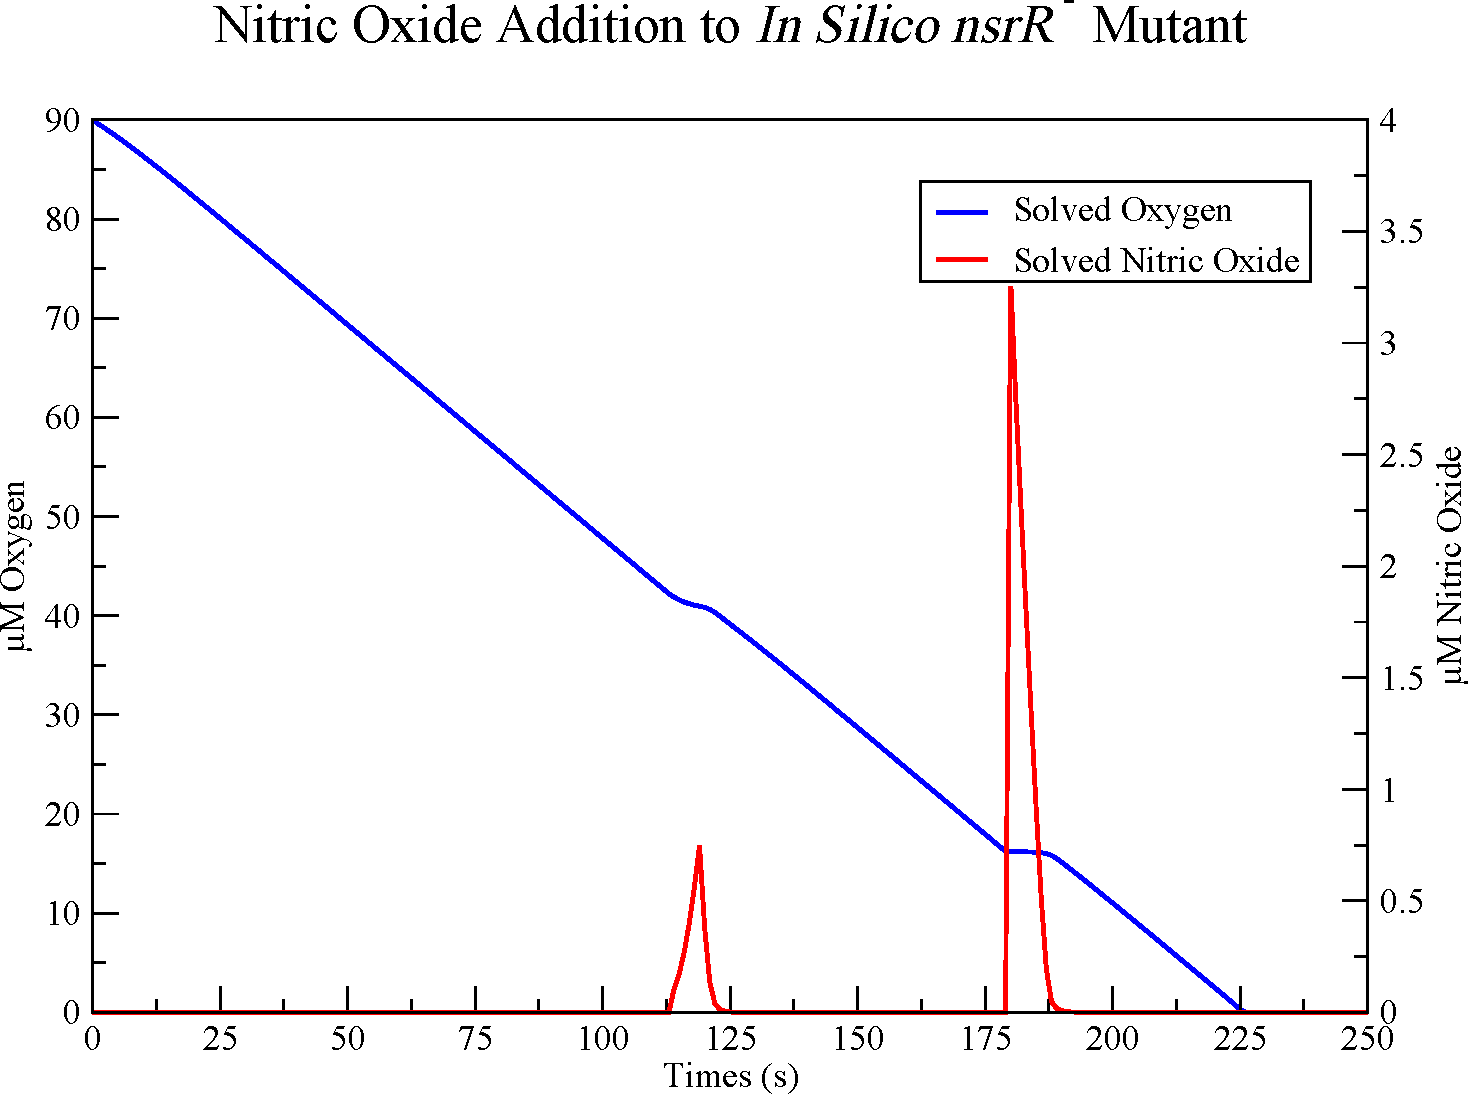
\includegraphics[width=15cm, clip=true]{./09-completedmodel/data/in_silico_nsrR.pdf}
 % in_silico_nsrR.pdf: 705x525 pixel, 72dpi, 24.87x18.52 cm, bb=0 0 705 525
 \caption[Nitric Oxide Addition to In silico nsrR Mutant]{{\bf Nitric Oxide Addition to \textit{In silico nsrR}$^-$ Mutant}. This figure shows the effect of adding two aliquots of increasing concentration of nitric oxide to a simulated $nsrR^-$ mutant.
 \label{fig:in_silico_nsrR}}
\end{figure}
This figure shows significant similarity with the experimentally observed result capturing the fast removal of nitric oxide due to the large quantities of NorB, and also models the slight reduction in oxygen reduction rate whilst the NO is being removed.

\subsection{\textit{In silico} cyt Knockouts}
It is possible to predict the effect on both the electron transport chain and the rates of respiration of knocking out some of the cytochromes that are encompassed within parameter $X$. This can be done by simply reducing the concentration of $X$ and leaving all other parameters unchanged. In this case the concentration was reduced by 25\% (this value is somewhat arbitrary but might be similar in effect knocking out 1 of the c-type cytochromes). This is a simplification of actually knocking out a specific cytochrome as this will actually affect all components downstream of $X$.

The experimental dataset used for comparison is that in Figure \ref{fig:nitrite_ds2_solved2}. The result of the simulated dataset is shown in Figure \ref{fig:in_silico_cyt} compared to the solved result from the wild-type.
\begin{figure}[tbp]
 \centering
 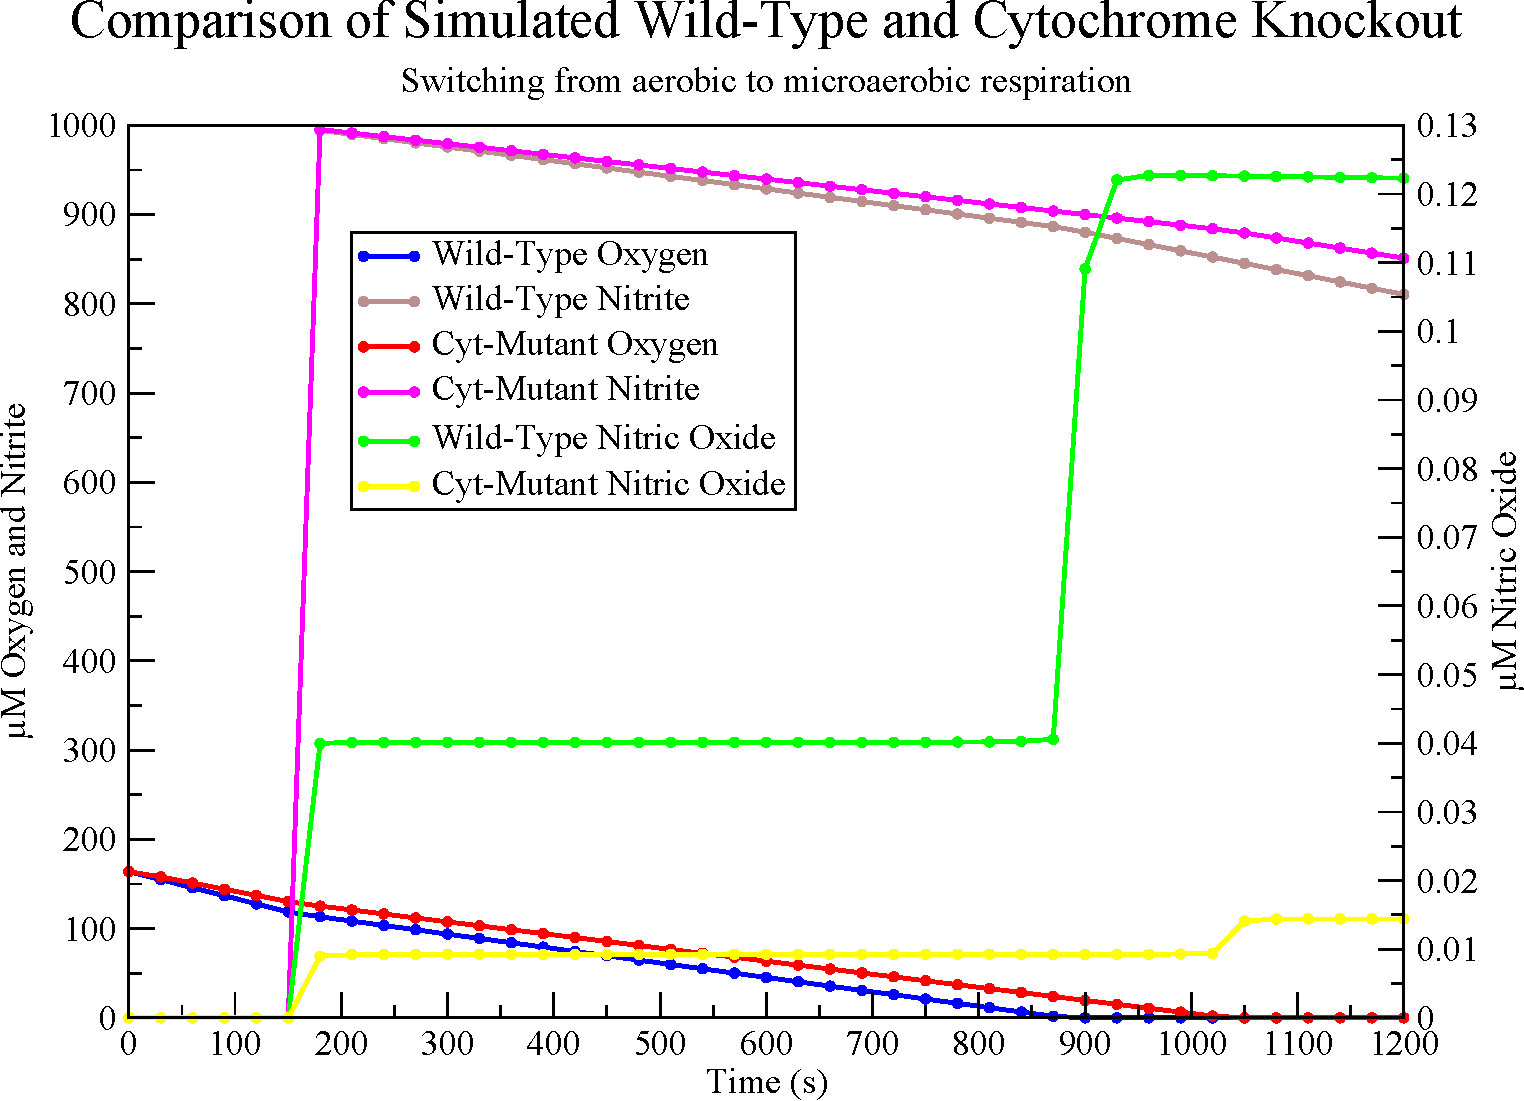
\includegraphics[width=15cm, clip=true]{./09-completedmodel/data/in_silico_cyt.pdf}
 % in_silico_nsrR.pdf: 705x525 pixel, 72dpi, 24.87x18.52 cm, bb=0 0 705 525
 \caption[In Silico Cytochrome Mutant]{{\bf \textit{In silico} Cytochrome Mutant}. This figure shows the effect of reducing the total amount of cytochromes while leaving all other components unchanged. All the reaction rates have slowed as a result of this change.
 \label{fig:in_silico_cyt}}
\end{figure}

The simulated cytochrome mutant shows that all reaction rates have slowed, although not by large amounts. The most obvious difference in the figure is the change in production and removal of nitric oxide, which is reduced to approximately 10\% of its production compared to the wild-type. This predicted result could easily be tested with an experiment using a c-type cytochrome knockout mutant grown in microaerobic conditions.

The reduction state plot can be seen in Figure \ref{fig:in_silico_cyt_redox}. It also compares the simulated cytochrome mutant to the wild-type. As can be seen, the redox states of \cbbthree{} and AniA do not change significantly as they are very efficient electron donors, remaining in an oxidised state. NorB remains in a more reduced state in the cytochrome mutant as there is less NO to ultimately reduce resulting in fewer electrons donated. The reduction state of the quinones is quite similar between the two simulations throughout. The reduction state of the cytochromes is significantly different, being higher than the wild-type at all times. This can be explained by looking at the quinone pool reduction state. As it remains fairly similar to the wild-type, the same flux of electrons must be passing through it, thus the same amount of electrons are being passed to fewer cytochromes. Since the rate of donation of electrons by the cytochromes has not been altered, the electrons build up in the cytochromes 
until a new steady-state is reached where the overall reduction state of the cytochromes is higher.

\begin{figure}[tbp]
 \centering
 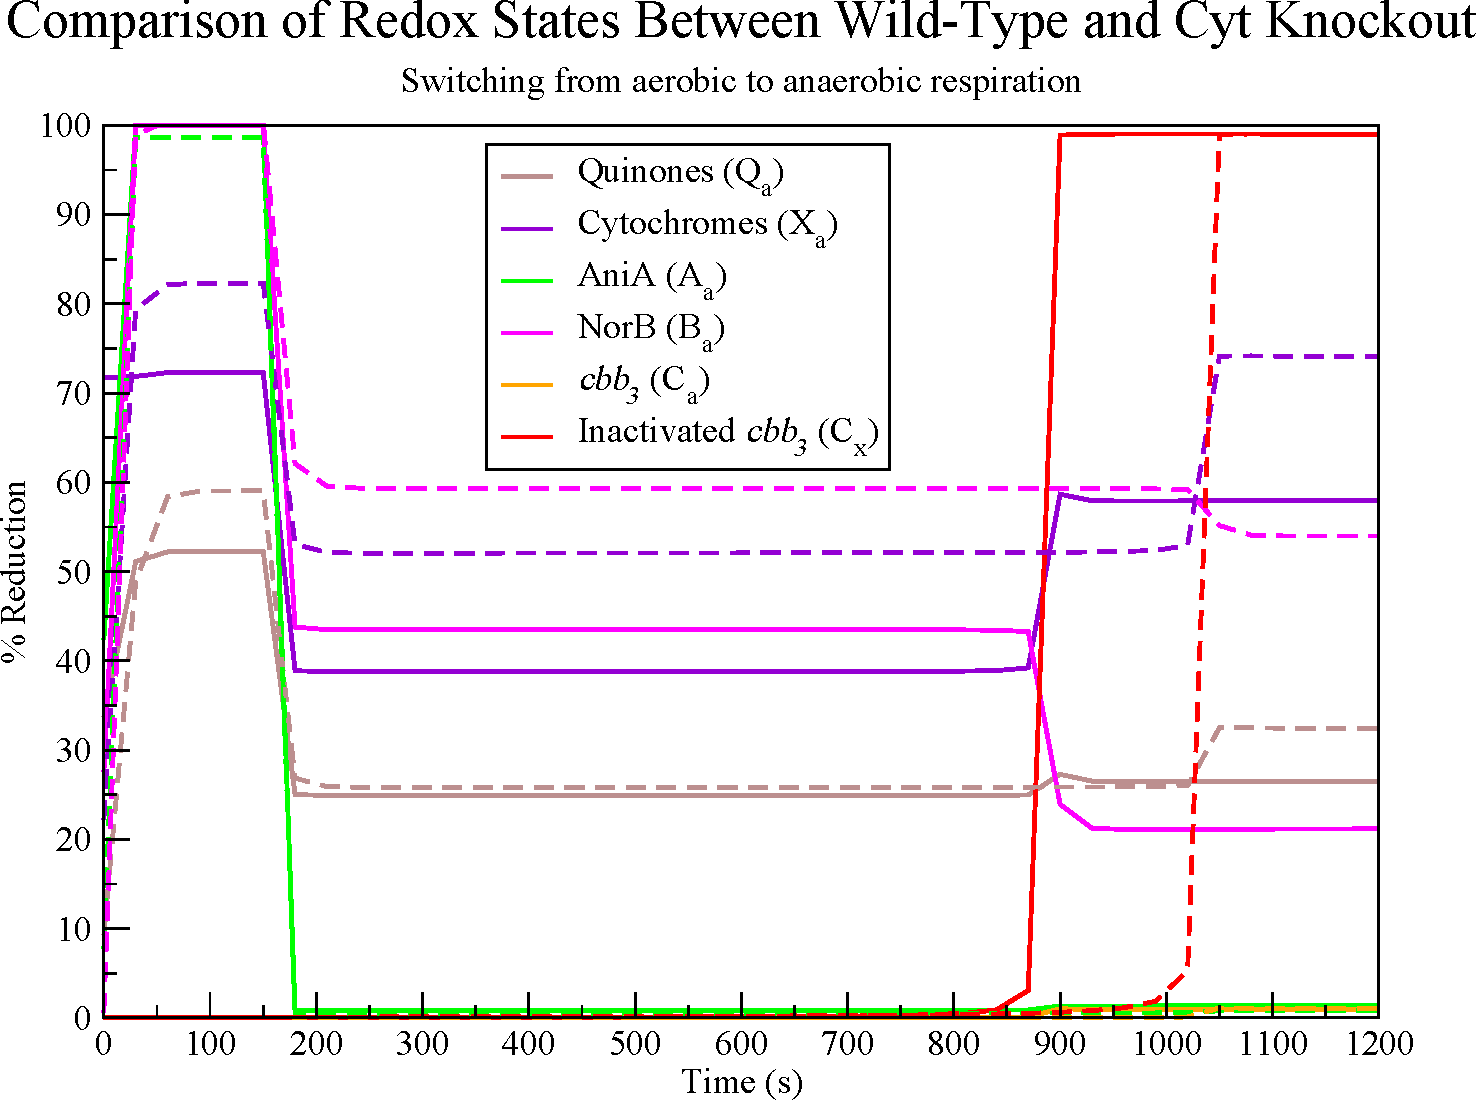
\includegraphics[width=15cm, clip=true]{./09-completedmodel/data/in_silico_cyt_redox.pdf}
 % in_silico_nsrR.pdf: 705x525 pixel, 72dpi, 24.87x18.52 cm, bb=0 0 705 525
 \caption[In Silico Cytochrome Mutant Redox States]{{\bf \textit{In silico} Cytochrome Mutant Redox States}. This figure shows the effect on the enzymatic reduction states of reducing the total number of cytochromes to simulate a cytochrome knockout mutant. The wild-type is represented by solid lines, and the synthetic mutant by dashed lines.
 \label{fig:in_silico_cyt_redox}}
\end{figure}

% \subsection{Electron Flux}
%
% \begin{eqnarray*}
% \mathrm{NADH~to~Quinone~rate~from~FBA} & = & 0.0173~Moles\cdot g^{-1}h^{-1}\\
% \times~2.8\times 10^{-13} g\cdot cell^{-1} & = & 4.844\times 10^{-15}~Moles\cdot cell^{-1}h^{-1}\\
% \div~3600~s\cdot h^{-1} & = & 1.35\times 10^{-18}~Moles\cdot cell^{-1}s^{-1}\\
% \div~1\times 10^{-15}~l\cdot cell^{-1} & = & 1.35\times 10^{-3} M\cdot s^{-1}\\
% \div~83\times 10^{-6}M & = & 16.3~s^{-1}
% \end{eqnarray*}

\section{Single Parameter Scaling Fits}
As has been discussed previously the proxy being used to try and estimate cell density appears to be inadequate as it does not scale correctly with the normalised data. It is however possible to obtain very good fits to all the experimental datasets with the exception of nitrite dataset 1 -  which is an $nsrR^-$ mutant - by simply introducing a ``scale factor'' which is applied to all concentrations in the system. An example of the better fit after using the scale factor is shown in Figure \ref{fig:improved_fit} in comparison to Figure \ref{fig:nitric_oxide_simulation}.

\begin{figure}[tbp]
 \centering
 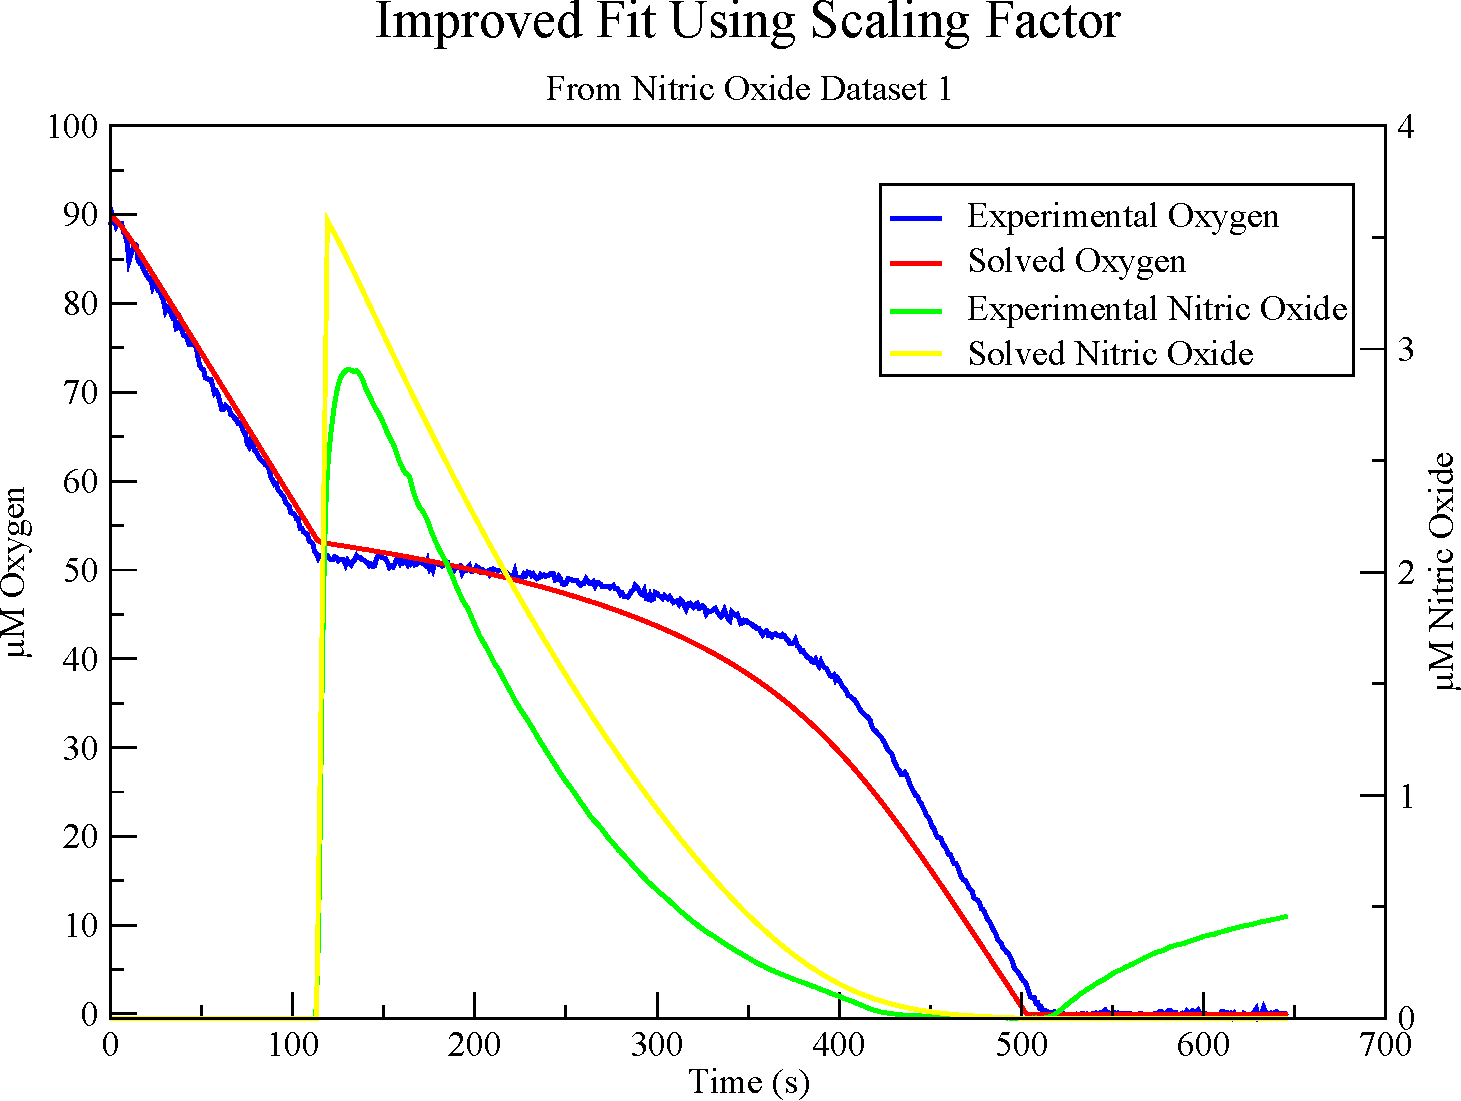
\includegraphics[width=15cm, clip=true]{./09-completedmodel/data/improved_fit.pdf}
 % in_silico_nsrR.pdf: 705x525 pixel, 72dpi, 24.87x18.52 cm, bb=0 0 705 525
 \caption[Improved Fit with Scaling Factor]{{\bf Improved Fit with Scaling Factor}. This figure shows the best fit achieved using a scaling factor rather than an approximate OD to calculate component concentrations. Compare with \ref{fig:nitric_oxide_simulation}.
 \label{fig:improved_fit}}
\end{figure}

The magnitude of the scale factor required for each dataset is shown in Table \ref{tab:scale-factors} along with the Oxygen Reduction Activity which formed part of the initial scaling.

\begin{table}[!ht]
\begin{center}
\begin{tabular}{ccc}
\toprule
Dataset & Scale Factor & $O_2$ Reduction Activity ($\mu Ms^{-1}$) \\
\midrule
Oxygen Dataset 1 & $\frac{1}{7}$ & 0.211027\\
\noalign{\smallskip}
Oxygen Dataset 2 & $\frac{1}{2.4}$ & 1.016159\\
\noalign{\smallskip}
Oxygen Dataset 3 & $\frac{1}{8}$ & 0.181488\\
\noalign{\smallskip}
Nitric Oxide Dataset 1 & $\frac{1}{5.5}$ & 0.336669\\
\noalign{\smallskip}
Nitric Oxide Dataset 3 & $\frac{1}{3}$ & 0.597478\\
\noalign{\smallskip}
Nitric Oxide Dataset 4 & $\frac{1}{5.8}$ & 0.324286\\
\noalign{\smallskip}
Nitrite Dataset 2 & $\frac{1}{5.8}$ (NorB $\frac{1}{5}$) & 0.275\\
\noalign{\smallskip}
\bottomrule
\end{tabular}
\end{center}
\caption{Dataset Scale Factors
\label{tab:scale-factors}}
\end{table}

The fact that NorB needed to be scaled by a smaller amount in Nitrite dataset 2 suggests that the value for NorB is actually underestimated in the priors. This does not affect the other datasets as they either have no NorB or only very low levels.

A plot of the scaling factors compared to the dataset oxygen reduction rates is shown in Figure \ref{fig:scaling-factors}. A simple linear regression through the datapoints suggests that the relationship between the two is approximately linear with a gradient of $0.36366$.

\begin{figure}[tbp]
 \centering
 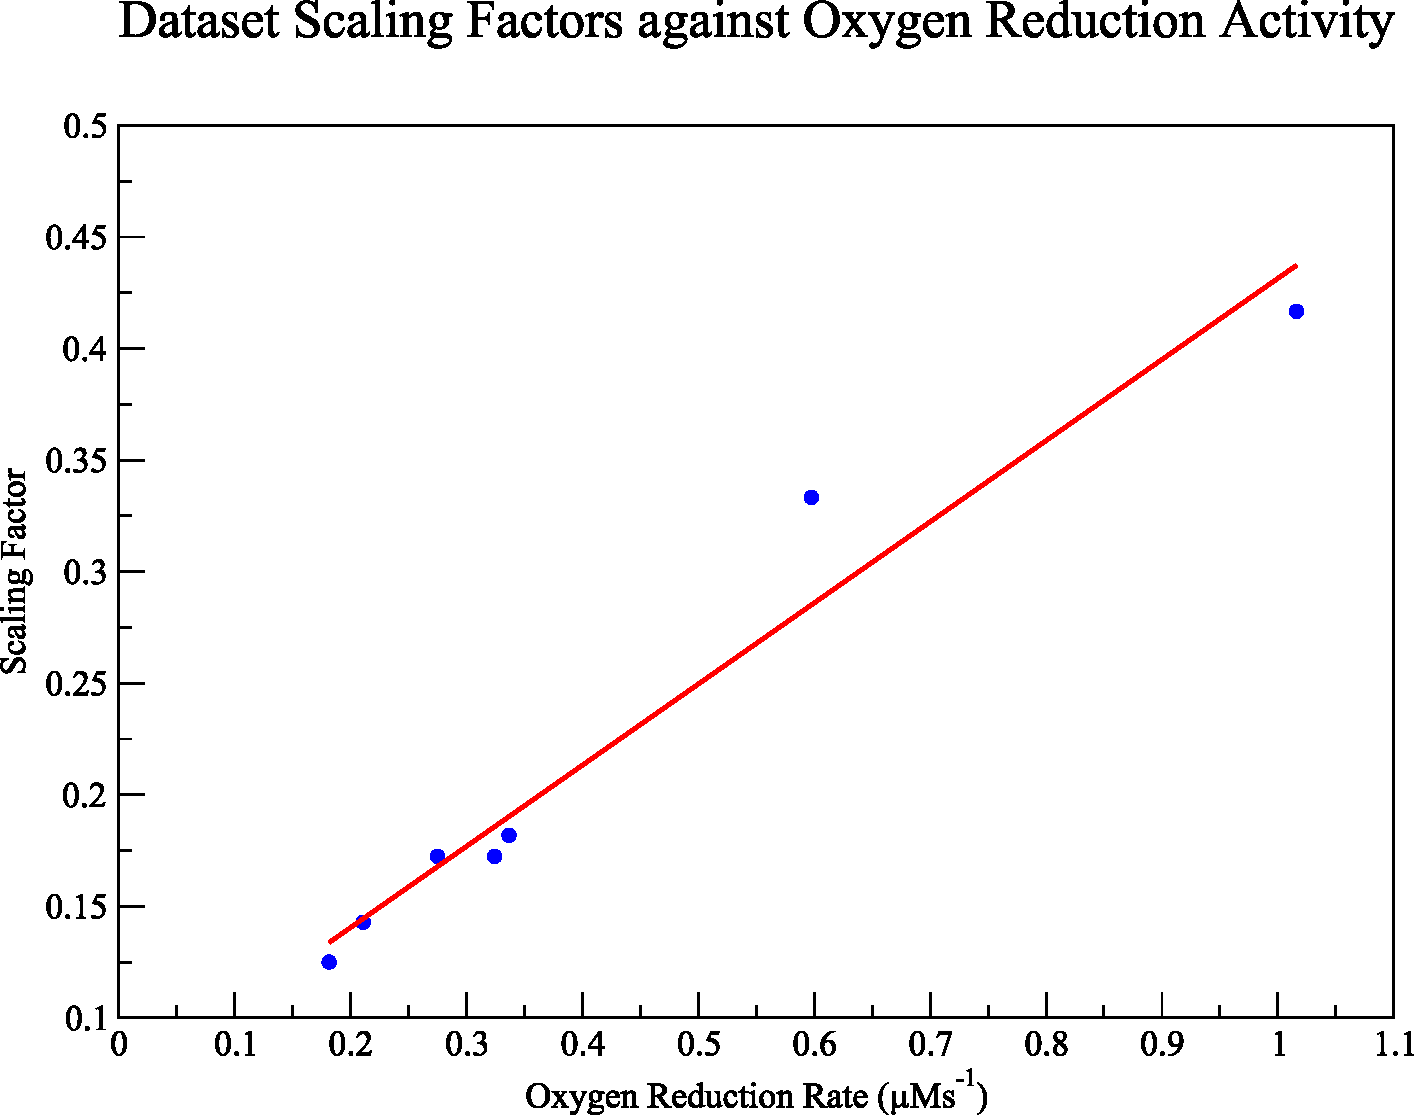
\includegraphics[width=15cm, clip=true]{./09-completedmodel/data/scaling.pdf}
 % in_silico_nsrR.pdf: 705x525 pixel, 72dpi, 24.87x18.52 cm, bb=0 0 705 525
 \caption[Dataset Scaling Factors]{{\bf Dataset Scaling Factors}. This figure shows the magnitude of the scaling factor relative to the experimental oxygen reduction rates. The red lines indicates a linear regression through the datapoints.
 \label{fig:scaling-factors}}
\end{figure}

\section{Concluding Remarks}
The parameterised model created in this work appears to be capable of at least qualitatively modelling the behaviour of all the datasets presented, using the final set of parameter distributions. The model is not 100\% quantitative, although this was not an explicit requirement for the model. It should still be capable of offering insight into how the system behaves even if it cannot predict changes precisely. The non-quantitative nature of the model was to be expected given the high level of complexity in the model and some of the assumptions made regarding cytochromes, backward reaction rates etc. The most obvious ``fault'' in the model is that there is an incomplete decoupling of cell density from other components. Unfortunately this is most probably because the proxy used was not completely accurate as a replacement for cell density.

The integrated parameter estimation system created for this work operates as intended and could be extended to parameterise other systems if the same Bayesian approach were taken to data gathering. It is not however a system that could be used without human curation though, as it can still produce mathematically correct results with parameters that are actually very unlikely \textit{in vivo}. This was shown in Chapter \ref{chap:nitritereduction} where the values for 2 parameters were an order of magnitude too high in the prior probability distributions causing the simulation to fail. These same values worked ``perfectly'' for the datasets in Chapters \ref{chap:oxygenreduction} and \ref{chap:noreduction}. Such human interaction with the system is important however as it forms part of the Bayesian approach whereby we provide the ``prior'' knowledge to the system.

In conclusion, a novel system for parametrising a respiration system model has been created and utilised which has been able to successfully populate the model and produce probability distributions for all parameters. These parameters are able to be used in a qualitative manner to match existing experimental data, and to provide insight into the hidden behaviour of the system. Such a novel system was necessary as no previous attempts at parameter estimation in a complex biological system have been able to produce the same richness of data as this approach simply due to the interactions between components in the model and the limited avenues of data gathering available for such a model.

\backmatter
\chapter{Appendix}

\newpage

\printnomenclature
%\printindex

\renewcommand{\bibname}{References}
\addcontentsline{toc}{chapter}{\bibname} 

\bibliography{/home/uncle_fungus/Documents/Resources/Work/bibtex-references/phd_refs}

\end{document}
